\documentclass[10pt]{memoir}
\setstocksize{220mm}{155mm} 	        
\settrimmedsize{220mm}{155mm}{*}	
\settypeblocksize{170mm}{116mm}{*}	
\setlrmargins{18mm}{*}{*}
\setulmargins{*}{*}{1.2}
%\setlength{\headheight}{5pt}%
\checkandfixthelayout[lines]
\linespread{1.16}
\flushbottom

%%% Hyphenation settings
\usepackage[htt]{hyphenat}
\hyphenation{he-lio-trope opos-sum}
\tracingparagraphs=1
%Hyphenation in Devanāgarī of the edition still missing? Probably this needs to be modified in babel-iast package? 

%%% babel
\usepackage[english]{babel}
\usepackage{babel-iast/babel-iast}

\babelfont[iast]{rm}[Renderer=Harfbuzz, Scale=1.3]{AdishilaSan}%AdishilaSan}
\babelfont[english]{rm}{Adobe Text Pro}

%%% more functionality
\PassOptionsToPackage{hyphens}{url}
\usepackage{hyperref}
\usepackage{pdflscape}
\usepackage{cleveref}
\usepackage{url}
\usepackage{cleveref}
\usepackage{microtype}
\usepackage{lineno}

%\usepackage{bigfoot}
%%% more functions
\usepackage[dvipsnames]{xcolor}
%\usepackage[para,perpage]{footmisc}

%%%für den Counter von Kapiteln und Sätzen! 
\newcommand{\uproman}[1]{\uppercase\expandafter{\romannumeral#1}}
\newcommand{\lowroman}[1]{\romannumeral#1\relax}

\makeindex
\newfontfamily\sanskritfont[Script=Devanagari,Mapping=RomDev,Scale=1.1]{Sanskrit2003}
\usepackage{pifont,fourier-orns,lettrine,psvectorian,paralist,enumitem,pdfpages,wrapfig,tabulary,lettrine,longtable}
\setlist[enumerate]{itemsep=0mm}
\usepackage[autostyle]{csquotes}
\usepackage[defaultlines=2,all]{nowidow}
\usepackage{ellipsis,adforn,booktabs,longtable,url,tikz}
\lineskiplimit=-3pt          

\makechapterstyle{IeT}{%
  \chapterstyle{default}
  \renewcommand*{\printchapternonum}{\centering}
  \renewcommand*{\clearforchapter}{\cleartorecto} 
  \aliaspagestyle{chapter}{empty}}
\chapterstyle{IeT}
\setsecnumdepth{none}  \openright  \nouppercaseheads
\settocdepth{subsubsection}

%%%% test better pagebreaks
%\def\fussy{%
%  \emergencystretch\z@
%  \tolerance 200%
%  \hfuzz .1\p@
%  \vfuzz\hfuzz}

%\interfootnotelinepenalty=10000\relax

%\usepackage[maxfloats=256]{morefloats}

%\maxdeadcycles=500

%raggedbottomsectiontrue
%%\checkandfixthelayout


%%%%%%%  biblatex
%\newcommand{\noun}[1]{\textsc{#1}}    %  philosophy-verbose
\usepackage[backend=biber, sorting=nyt, style=verbose]{biblatex} %%%%ORIGINAL TiE
\renewcommand*{\mkbibnamefamily}[1]{\textsc{#1}}


\DeclareFieldFormat{url}{%
  \mkbibacro{URL}\addcolon\space
  \href{#1}{\nolinkurl{\thefield{urlraw}}}}

\DeclareFieldFormat{citeurl}{%
  \href{#1}{\nolinkurl{\thefield{urlraw}}}} 


\DeclareFieldFormat{postnote}{#1}
\renewcommand{\postnotedelim}{, }
\addbibresource{bindu.bib}

%%% ekdosis
\usepackage[teiexport=tidy,parnotes=true]{ekdosis}% =tidy cleans up HTML and XML documents by fixing markup errors and upgrading legacy code to modern standards. parnotes=footnotes below or above critical apparatus

\SetLineation{lineation=page, modulo} %lineation=page sets thenumbering to start afresh at the top of each page. =modulo makes every fifth line numbered. {lineation=page} makes every line numbered! 

\renewcommand{\linenumberfont}{\selectlanguage{english}\footnotesize} %sets language of lines to English

\SetTEIxmlExport{autopar=false} %autopar=falseinstructs ekdosis to ignore blank lines in the.tex sourcefile as markers for paragraph boundaries. As a result, each paragraph of the edition must be found within an environment associated with the xml <p> element

\SetHooks{
  lemmastyle=\bfseries,
  %refnumstyle=\selectlanguage{english}\bfseries,
  refnumstyle=\selectlanguage{english}\color{blue}\bfseries,
  appheight=0.8\textheight,
}

\newif\ifinapparatus
\DeclareApparatus{source}[
%bhook=\inapparatustrue,
lang=english,
notelang=english,
% bhook=\selectlanguage{english},
bhook=\selectlanguage{english}\textbf{Sources:},%
%maxentries=4, 
%ehook=.]
%sep={] },
%nosep,
]

\newif\ifinapparatus
\DeclareApparatus{testium}[
%bhook=\inapparatustrue,
lang=english,
notelang=english,
% bhook=\selectlanguage{english},
bhook=\selectlanguage{english}\textbf{Testimonia:},
%maxentries=4, 
%ehook=.]
%nosep, 
]

% Declare \ifinapparatus and set \inapparatustrue at the beginning of
% the apparatus criticus block. Also set the language.  
\newif\ifinapparatus
  \DeclareApparatus{default}[
  %bhook=\inapparatustrue, 
  lang=english,
  %maxentries=33,
  %bhook=\selectlanguage{english},
  sep = {] },
  delim=\hskip 0.75em,
  rule=\rule{0.7in}{0.4pt},
]

\newif\ifinapparatus
\DeclareApparatus{philcomm}[
%bhook=\inapparatustrue,
lang=english,
notelang=english,
bhook=\selectlanguage{english}\textbf{Philological Commentary:},
%bhook=\selectlanguage{english},
sep={: },
]

\ekdsetup{
showpagebreaks,
spbmk = \textcolor{blue}{spb},
hpbmk = \textcolor{red}{hpb}
}

%\usepackage{fnpos}
%\makeFNmid
%\makeFNbottom
\usepackage[bottom]{footmisc}
%%%%%%%%%%%%%%%%%%%%%%%%%%%
\makeatletter
\def\blfootnote{\gdef\@thefnmark{}\@footnotetext}
\makeatother
%%%%%%%%%%%%%%%%%%%%%%%%%


% Macros and Definitions for the Print of Sigla
\def\acpc#1#2#3{{#1}\rlap{\textrm{\textsuperscript{#3}}}\textsubscript{\textrm{#2}}\space}
\def\sigl#1#2{{{#1}}\textsubscript{\textrm{#2}}}
\def\None{{\sigl{N}{1}}} \def\Noneac{\acpc{N}{1}{ac}\,} \def\Nonepc{\acpc{N}{1}{pc}\,}
\def\Ntwo{{\sigl{N}{2}}} \def\Noneac{\acpc{N}{2}{ac}\,} \def\Nonepc{\acpc{N}{2}{pc}\,}
\def\Done{{\sigl{D}{1}}} \def\Doneac{\acpc{D}{1}{ac}\,} \def\Donepc{\acpc{D}{1}{pc}\,}
\def\Dtwo{{\sigl{D}{2}}} \def\Dtwoac{\acpc{D}{2}{ac}\,} \def\Dtwopc{\acpc{D}{2}{pc}\,}
\def\Uone{{\sigl{U}{1}}} \def\Uoneac{\acpc{U}{1}{ac}\,} \def\Uonepc{\acpc{U}{1}{pc}\,}                 
\def\Utwo{{\sigl{U}{2}}} \def\Utwoac{\acpc{U}{2}{ac}\,} \def\Utwopc{\acpc{U}{2}{pc}\,}

%%%%%%%%%%%%%% Tattvabinduyoga - List of Witnesses   %%%%%%%%%%%%%%%%%%%
\DeclareWitness{ceteri}{\selectlanguage{english}cett.}{ceteri}[]   
\DeclareWitness{E}{\selectlanguage{english}E}{Printed Edition}[]    
\DeclareWitness{P}{\selectlanguage{english}P}{Pune BORI 664}[]  
\DeclareWitness{B}{\selectlanguage{english}B}{Bodleian 485}[]       
\DeclareWitness{N1}{\selectlanguage{english}N\textsubscript{1}}{NGMPP 38/31}[]
\DeclareWitness{N2}{\selectlanguage{english}N\textsubscript{2}}{NGMPP B 38/35}[]
\DeclareWitness{L}{\selectlanguage{english}L}{LALCHAND 5876}[]  
\DeclareWitness{D}{\selectlanguage{english}D}{IGNCA 30019}[] 
%\DeclareWitness{D2}{\selectlanguage{english}D\textsubscript{2}}{IGNCA 30020}[]  
\DeclareWitness{U1}{\selectlanguage{english}U\textsubscript{1}}{SORI 1574}[] 
\DeclareWitness{U2}{\selectlanguage{english}U\textsubscript{2}}{SORI 6082}[]
%%%%%%%%%%%%%% Tattvabinduyoga - Groups of Witnesses   %%%%%%%%%%%%%%%%%%%
\DeclareWitness{X}{\selectlanguage{english}\alpha}{Alpha Group: D,N1,N2,U1}[]
\DeclareWitness{Y}{\selectlanguage{english}\beta}{Beta Group: B,E,L,P,U2}[]
%%%%%%%%%%%%% Testimonia
\DeclareWitness{Ysv}{\selectlanguage{english}Ysv}{Yogasvarodaya}[] %%%add infos!  

%%%%%%%%%%%%%%%%%%%%%%%%%%%%%%%%%%%%%%%%%%%
% Macro for Editing Abbrevs.
\def\om{\textrm{\footnotesize \textit{om.}\ }} %prints om. for omitted in apparatus
\def\korr{\textrm{\footnotesize \textit{em.}\ }} %prints em. for emended in apparatus
\def\conj{\textrm{\footnotesize \textit{conj.}\ }} %prints conj. for conjectured in apparatus

% \supplied{text} EDITORIAL ADDITION -> Within \lem oder \rdg
% \surplus{text} EDITORIAL DELETION -> Within \lem oder \rdg
% \sic{text} CRUX
% \gap{text} LACUNAE -> [reason=??, unit=??, quantity=??, extent=??]


%%%%%%%%%%%%%%%%%%%%%%%%%%%%%%%%%%%%%%%%%%% All macros of this list can be used in 
% Macro for Editing Abbrevs.
\def\eyeskip{\textrm{{ab.\,oc. }}}
\def\aberratio{\textrm{{ab.\,oc. }}}
\def\ad{\textrm{{ad}}}
\def\add{\textrm{{add.\ }}}
\def\ann{\textrm{{ann.\ }}}
\def\ante{\textrm{{ante }}} 
\def\post{\textrm{{post }}}
%\def\ceteri{cett.\,}                   
\def\codd{\textrm{{codd.\ }}}

\def\coni{\textrm{{coni.\ }}}
\def\contin{\textrm{{contin.\ }}}
\def\corr{\textrm{{corr.\ }}}
\def\del{\textrm{{del.\ }}}
\def\dub{\textrm{{ dub.\ }}}

\def\expl{\textrm{{explic.\ }}} 
\def\explica t{\textrm{{explic.\ }}}
\def\fol{\textrm{{fol.\ }}}
\def\foll{\textrm{{foll.\ }}}
\def\gloss{\textrm{{glossa ad }}}
\def\ins{\textrm{{ins.\ }}}      
\def\inseruit{\textrm{{ins.\ }}} 
\def\im{{\kern-.7pt\lower-1ex\hbox{\textrm{\tiny{\emph{i.m.}}}\kern0pt}}} %\textrm{\scriptsize{i.m.\ }}}      
\def\inmargine{{\kern-.7pt\lower-.7ex\hbox{\textrm{\tiny{\emph{i.m.}}}\kern0pt}}}%\textrm{\scriptsize{i.m.\ }}}      
\def\intextu{{\kern-.7pt\lower-.95ex\hbox{\textrm{\tiny{\emph{i.t.}}}\kern0pt}}}%\textrm{\scriptsize{i.t.\ }}}           
\def\indist{\textrm{{indis.\ }}}  
\def\indis{\textrm{{indis.\ }}}
\def\iteravit{\textrm{{iter.\ }}} 
\def\iter{\textrm{{iter.\ }}}
\def\lectio{\textrm{{lect.\ }}}   
\def\lec{\textrm{{lect.\ }}}
\def\leginequit{\textrm{{l.n. }}} 
\def\legn{\textrm{{l.n. }}}
\def\illeg{\textrm{{l.n. }}}

\def\primman{\textrm{{pr.m.}}}
\def\prob{\textrm{{prob.}}}
\def\rep{\textrm{{repetitio }}}
\def\secundamanu{\textrm{\scriptsize{s.m.}}}            \def\secm{{\kern-.6pt\lower-.91ex\hbox{\textrm{\tiny{\emph{s.m.}}}\kern0pt}}}%   \textrm{\scriptsize{s.m.}}}
\def\sequentia{\textrm{{seq.\,inv.\ }}}  
\def\seqinv{\textrm{{seq.\,inv.\ }}}
\def\order{\textrm{{seq.\,inv.\ }}}
\def\supralineam{{\kern-.7pt\lower-.91ex\hbox{\textrm{\tiny{\emph{s.l.}}}\kern0pt}}} %\textrm{\scriptsize{s.l.}}}
\def\interlineam{{\kern-.7pt\lower-.91ex\hbox{\textrm{\tiny{\emph{s.l.}}}\kern0pt}}}   %\textrm{\scriptsize{s.l.}}}
\def\vl{\textrm{v.l.}}   \def\varlec{\textrm{v.l.}} \def\varialectio{\textrm{v.l.}}
\def\vide{\textrm{{cf.\ }}}
\def\cf{\textrm{{cf.\ }}} 
\def\videtur{\textrm{{vid.\,ut}}}
\def\crux{\textup{[\ldots]} }
\def\cruxx{\textup{[\ldots]}}
\def\unm{\textit{unm.}}
%%%%%%%%%%%%%%%%%%%%%%%%%%%%%%%%%%%%

% List of Scholars
\DeclareScholar{ego}{ego}[
forename=Nils Jacob,
surname=Liersch]

% Persons:14\DeclareScholar{ego}{ego}[15forename=Robert,16surname=Alessi]17% Useful shorthands:18\DeclareShorthand{codd}{codd.}{V,I,R,H}19\DeclareShorthand{edd}{edd.}{Lit,Erm,Sm}20\DeclareShorthand{egoscr}{\emph{scripsi}}{ego}

%Useful shorthands:
%\DeclareShorthand{codd}{codd.}{V,I,R,H}
%\DeclareShorthand{edd}{edd.}{Lit,Erm,Sm}
\DeclareShorthand{egoscr}{em.}{ego}
\DeclareShorthand{egoscrconj}{conj.}{ego}
\DeclareShorthand{egomute}{\unskip}{ego}

\usepackage{xparse}

\NewDocumentEnvironment{tlg}{O{}O{}}{\setlength{\leftskip}{0pt}\vspace{-1ex}\begin{quotation}}{\hfill #1\ \vspace{-1ex}\end{quotation}\vspace{-1ex}} %verse environment
%\NewDocumentEnvironment{tlg}{O{}O{}}{\begin{verse}}{॥#1\hskip-4pt ॥\\ \end{verse}}
\NewDocumentCommand{\tl}{m}{{\selectlanguage{iast} #1}}

\NewDocumentCommand{\extra}{m}{{\textcolor{gray}{#1}}} %command for additions to U2
\NewDocumentCommand{\crazy}{m}{{\textcolor{red}{#1}}} %totally corrupted passage
\NewDocumentCommand{\coro}{m}{{\textcolor{violet}{#1}}} %colour for sentence counter! 

\NewDocumentEnvironment{prose}{O{}}{\begin{otherlanguage}{iast}}{\end{otherlanguage}}
% \NewDocumentEnvironment{padd}{O{}}{\begin{otherlanguage}{iast}}{\end{otherlanguage}}
\NewDocumentEnvironment{tlate}{O{}}
%\NewDocumentEnvironment{tadd}{O{}}

%Define two commands: \skp ("sanskrit plus"), to be ignored by TeX in
%the edition text, but processed in the TEI output. Conversely, \skm
%("sanskrit minus") is to be processed in the edition text, but
%ignored if found in the apparatus criticus and in the TEI output:

\NewDocumentCommand{\skp}{m}{}
\TeXtoTEIPat{\skp {#1}}{#1}

%\NewDocumentCommand{\skpp}{m}{}
%\TeXtoTEIPat{\skpp {#1}}{#1}

\NewDocumentCommand{\skm}{m}{\unless\ifinapparatus#1-\fi}
\TeXtoTEIPat{\skm {#1}}{}

% \NewDocumentCommand{\dd}{}{/\hskip-4pt/}
\NewDocumentCommand{\dd}{}{\mbox{/\hskip-4pt/}}
\TeXtoTEIPat{\dd {}}{//}


%%% modify environments and commands
%%% TEI mapping
\TeXtoTEIPat{\begin {tlg}}{<lg>} %lg=(Group of verse (s)) contains one or more verses or lines of verse that together form a formal unit (e.g. stanza, chorus).
\TeXtoTEIPat{\end {tlg}}{</lg>}

\TeXtoTEIPat{\begin {prose}}{<p>}
\TeXtoTEIPat{\end {prose}}{</p>}

\TeXtoTEIPat{\begin {tlate}}{<p>}
\TeXtoTEIPat{\end {tlate}}{</p>}

\TeXtoTEIPat{\\}{}
\TeXtoTEIPat{\linebreak}{<br/>}
\TeXtoTEIPat{\noindent}{}
%\TeXtoTEI{tl}{l}
\TeXtoTEI{emph}{hi}
\TeXtoTEI{bigskip}{}
\TeXtoTEI{None}{N1}
\TeXtoTEI{Ntwo}{N2}
\TeXtoTEI{Done}{D1}
\TeXtoTEI{Dtwo}{D2}
\TeXtoTEI{Uone}{U1}
\TeXtoTEI{Utwo}{U2}
%\TeXtoTEIPat{/}{ |}
%\TeXtoTEI{//}{ ||}
\TeXtoTEIPat{\korr}{em. }
\TeXtoTEIPat{\conj}{conj.}
\TeXtoTEIPat{\om}{om.}
\TeXtoTEIPat{english}{}
\TeXtoTEIPat{\hskip}{}
\TeXtoTEIPat{\hskip-4pt}{}
\TeXtoTEIPat{\hskip-2pt}{}
\TeXtoTEIPat{-}{ }
\TeXtoTEIPat{4pt}{}
\TeXtoTEIPat{2pt}{}
\TeXtoTEIPat{\textcolor {#1}{#2}}{<hi rend="#1">#2</hi>} 

% Nullify \selectlanguage in TEI as it has been used in
% \DeclareWitness but should be ignored in TEI.
\TeXtoTEI{selectlanguage}{}



\FormatDiv{1}{\begin{center}\Large}{\end{center}}
\FormatDiv{2}{\begin{center}\small}{\end{center}}
\FormatDiv{3}{\bfseries}{.}
\title{Yogatattvabindu of Rāmacandra\\ A Critical Edition and Annotated Translation}
\date{\today}

\parindent=15pt
\begin{document}

%Zitiermöglichkeiten:
%\footcite[See][p.\,1]{goldstein01:_tibet_englis_diction_moder_tibet}
%\footnote{\cite{goldstein01:_tibet_englis_diction_moder_tibet}.}

\frontmatter
\thispagestyle{empty}
\begin{center}
  {\Large \emph{The Yogatattvabindu}}\\[3mm]
\end{center}



\newpage

\

\thispagestyle{empty}



\normalsize


\newpage


\begin{center}
\thispagestyle{empty}

\

\vskip 2mm

\begin{otherlanguage}{iast}
\LARGE \sanskritfont{Yogatattvabindu}
\end{otherlanguage}

\vskip .4cm

\Huge Yogatattvabindu \\[7mm]
\Large Critical Edition\\
and annotated Translation\\
together with a Comparative Analysis of the \\Complex Early Modern Yoga Yaxonomies 


\large

\vspace{3cm}

By

Nils Jacob Liersch
\small
\vfill

\vfill

Indica et Tibetica Verlag \\ % $\cdot$ 
Marburg 2024

\vskip 6mm

\end{center}

\newpage
\newpage \ \thispagestyle{empty}
\small  \

\noindent

\
\vfill


\small
\noindent \textbf{Bibliographische Information Der Deutschen Bibliothek}

\noindent
Die Deutsche Bibliothek verzeichnet diese Publikation in der Deutschen Nationalbibliographie;
detaillierte bibliographische Informationen sind im Internet über http://dnb.ddb.de abrufbar.

\noindent
\textbf{Bibliographic information published by Die Deutschen Bibliothek}

\noindent
Die Deutsche Bibliothek lists this publication in the Deutsche Nationalbibliographie; detailed
bibliographic data is available in the Internet at http://dnb.ddb.de.  


\vskip 1cm

\noindent
\copyright\ Indica et Tibetica Verlag, Marburg 2024

\medskip

\noindent
Alle Rechte vorbehalten / All rights reserved

\medskip

\noindent
Ohne ausdrückliche Genehmigung des Verlages ist es nicht gestattet, das Werk oder einzelne Teile
daraus nachzudrucken, zu vervielfältigen oder auf Datenträger zu speichern.

\smallskip

\noindent
Apart from any fair dealing for the purpose of private study, research, criticism or review, no
part of this book may be reproduced or translated in any form, by print, photo form, microfilm, or
any other means without written permission. Enquiries should be made to the publishers.

\bigskip

\noindent
Satz: \ \ Nils Jacob Liersch \\
Herstellung: \ \ BoD – Books on Demand GmbH, Norderstedt  \\

\bigskip

\noindent
%\ISBN     

\normalsize

\newpage

%\maketitle
\clearpage
\tableofcontents
\addtocounter{page}{-1}
\thispagestyle{empty}
\clearpage


\mainmatter

\chapter{Conventions in the Critical Apparatus}
\section{Sigla in the Critical Apparatus}

\begin{itemize}
\item E : Printed Edition
\item P : Pune BORI 664
\item L : Lalchand Research Library LRL5876
\item B : Bodleian Oxford D 4587
‚\item \None : NGMPP B 38-31
\item \Ntwo : NGMPP B 38-35 / A 1327-14
\item \Done : IGNCA 30019
\item \Uone : SORI 1574
\item \Utwo : SORI 6082
\end{itemize}

\chapter{Critical Edition \& Annotated Translation}
\cleardoublepage
\begin{alignment}[
  texts=edition[class="edition"];
  translation[class="translation"],
  ]
  \begin{edition}
\ekddiv{
  head={[\uproman{40}. \textbf{śarīre navanāḍyaḥ}]},
  type=section,
  depth=2, 
  n=XL
}
\xmlhead[h40]{[XL. śarīre navanāḍyaḥ]}
\label{ninerivers}
    \begin{prose}[p40_01]
      \noindent
%----------------------------
%idānīṃ śarīramadhye navanāḍyas tiṣṭhanti   tanmadhye navanadīnāṃ     sthānāni   varttante/   \E
%idānīṃ śarīre       navanaḍyas tiṣṭhaṃti   tanmadhye navāṃnā nadīnāṃ sthānāni   vartaṃte     \P
%idānīṃ śarīre       navanaḍyas tiṣṭhanti// tanmadhye navānāṃ nadīnāṃ sthānāni   vartate/     \B
%idānīṃ śarīre       navanaḍyaḥ tiṣṭhaṃti/  tanmadhye navānāṃ nadīnāṃ sthānāni   vartaṃte/    \L
%\om                                                                 \N1
%idānīṃ śarīre       ṇavānāḍyas tiṣṭhati//  tanmadhye navānāṃ nadīnāṃ sthānāni   vartraṃte//  \D
%\om                                                                 \N2
%idānīṃ śarīre       ṇavānaḍyaḥ stiṣṭhaṃti  tanmadhye navānāṃ nadīnāṃ sthānāni   vartaṃte    \U1
%idānīṃ śarīramadhye navanāḍyas tiṣṭhati//  tanmadhye navānāṃ nadīnāṃ          nivarttaṃte// \U2
%-----------------------------
%Now, within the body there are nine rivers. Within it the courses of the nine rivers exist. 
%----------------------------
      \note[type=source, labelb=284, labele=_284e, nosep]{cf. YSv (PT p. 843): śarīre navanāḍīsthā narmadā ca maheśvari | iḍāyāṃ yamunā devi piṅgalāyāṃ sarasvatī | suṣumnāyāṃ vahed gaṅgā cānyonyāsu ca nāḍiṣu | gaṅgā sarasvatī godā narmadā yamunā tathā | kāverī candrabhāgā ca vitastā ca iḍāvatī | dvisaptatisahasreṣu nadīnadaparisravaḥ |}
      \note[type=source, labelb=283, labele=_284e, nosep]{cf. SSP 3.11-12 (Ed. p. 57): pīnasā yamunā gaṅgā candrabhāgā sarasvatī | vipāsā śatarudrā ca śrīrātriś caiva narmadā | evaṃ navanadyo navanāḍīṣu vasanti | anyā upanadyaḥ kulyopakulyā dvisaptatisahasranāḍīsu vasanti |}
idānīṃ
\app{\lem[wit={ceteri}]{śarīre}
  \rdg[wit={E,U2}]{śarīramadhye}}
\app{\lem[wit={E,U2},alt={navanāḍyas}]{navanāḍya\skp{s-ti}}
  \rdg[wit={B,L,P}]{navanaḍyas}
  \rdg[wit={D}]{ṇavānāḍyas}
  \rdg[wit={U1}]{ṇavānaḍyaḥs}}
\app{\lem[wit={ceteri}, alt={tiṣṭhanti}]{\skp{s-ti}ṣṭhanti}
  \rdg[wit={D,U2}]{tiṣṭhati}}/
tanmadhye
\app{\lem[wit={ceteri}]{navānāṃ nadīnāṃ}
  \rdg[wit={E}]{navanadīnāṃ}}
sthānāni
\app{\lem[wit={ceteri}]{vartante}
  \rdg[wit={U2}]{nivartaṃte}
  \rdg[wit={B}]{vartate}}/
%----------------------------     
%gaṃgāyamune vitastā candrabhāgā sarasvatī vipāśā   śatahradā   irāvatī narmadā/   \E [p.52]
%gaṃgāyamunā vitastā caṃdrabhāgā sarasvatī vipāśā   śātahṛdā    irāvati narmmadā    \P
%gaṃgāyamunā vitastā caṃdrabhāgā sarasvatī vipāśā   śāśatahṛdā  irāvati narmadā/  \B
%gaṃgāyamunā vitastā caṃdrabhāgā sarasvati vipāśā   śatat hṛda  irāvati narmadā// \L
%\om                                                                 \N1
%gaṃgāyamunā vitastā caṃdrabhāgā sarasvatī/ vaipaśā śata hṛdā// irāvatī/ narmadā/ \D
%\om                                                                 \N2
%gaṃgāyamunā vitastā caṃdrabhāgā sarasvatī vaipaśā  śata hṛdā   airāvati narmadā \U1
%gaṃgāyamunā vitastā candrabhāgā sarasvatī vipāśā   śātadrumā//          narmadā   \U2
%-----------------------------
%Gaṅga, Yamuna, Vitastā, Candrabhāga, Sarasvatī, Vipāśā, Śatarudrā, Irāvati und Narmadā.  
%-----------------------------
gaṅgā yamunā vitastā caṃdrabhāgā
\app{\lem[wit={ceteri}]{sarasvatī}
  \rdg[wit={L}]{sarasvati}}
\app{\lem[wit={ceteri}]{vipāśā}
  \rdg[wit={D,U1}]{vaipaśā}}
\app{\lem[type=emendation, resp=egoscr]{śatarudrā}
  \rdg[wit={D,P,U1}]{śātahṛdā}
  \rdg[wit={E}]{śatahradā}
  \rdg[wit={B}]{śāśatahṛdā}
  \rdg[wit={U2}]{śātadrumā}}
%\note[type=philcomm, labelb=285, lem={śatarudrā}]{I emended according to YSv (PT).}
\app{\lem[wit={D,E}]{irāvatī}
  \rdg[wit={B,L,P,U1}]{irāvati}
  \rdg[wit={U2}]{\om}}
narmadā/ 
%-----------------------------
%aparā    nadyo    nadāni       srotāṃsi   taṭākāni  vāpīkūpā---disaptati----sahasranāḍī----madhye tiṣṭhanti/  \E
%aparā    nadyo    nadānir jārā srotāṃsī   taṭānī    vāpīkūpā---dvisaptatī---sahasranāḍīnāṃ madhye tiṣṭaṃti    \P %7660.jpg
%aparā    nadyo    nadānir jñārāsty etāṃsī taṭānī    vāpīkūpā---dvisaptatī---sahasranāḍīnā--madhye tiṣṭaṃti/   \B
%aparā    nadyo    nadānir jñārāsty etāṃsi taṭāni    vāpīkūpā---dvisaptati---sahasranāḍīnāṃ madhye tiṣṭaṃti/   \L
%\om                                                                                                   \N1
%aparā    nadyopanadīnair   bhurasrota-----taṭāka----vāpikupāḥ  dvisaptati---sahasranāḍīnāṃ madhye tiṣṭaṃti/  \D
%\om                                                                                                   \N2
%gaṃḍakī  nadyūpanadīnair  bhurasrota------taḍaga    vāpīkūpa---dvisaptati---sahastranāḍī   madhye  tiṣṭhaṃṭī  \U1  %em zu upanadinirjhara!!! Wasserfälle! 
%aparā    nadyo   nadānir  jñārāsrotāsī    taṭhānī   vāpīkūpā---dvisaptati---sahasranāḍīnāṃ madhye tiṣṭaṃti//  \U2
%-----------------------------
%Other rivers, and waterfalls near the rivers, currents, lakes, ponds and wells are situated within the 72000 channels.
%-----------------------------
\app{\lem[wit={ceteri}]{aparā}
  \rdg[wit={U1}]{gaṃḍakī}}
\app{\lem[type=emendation, resp=egoscr]{nadyopanadinirjharāḥ srotāṃsi}
    \rdg[wit={D}]{nadyopanadīnair bhurasrota°}
    \rdg[wit={U1}]{nadyūpanadīnair bhurasrota°}
    \rdg[wit={P}]{nadyo nadānirjārā srotāṃsī}
    \rdg[wit={B,L}]{nadyo nadānirjñārāsty etāṃsī}
    \rdg[wit={U2}]{nadyo nadānirjñārāsrotāsī}
    \rdg[wit={E}]{nadyo nadāni srotāṃsi}}
\app{\lem[wit={E}]{taṭākāni}
    \rdg[wit={D}]{taṭāka}
    \rdg[wit={B,L,P}]{taṭānī}
    \rdg[wit={U1}]{taḍaga}
    \rdg[wit={U2}]{taṭhānī}}
\app{\lem[wit={ceteri}]{vāpīkūpā}
  \rdg[wit={D}]{vāpikupāḥ}}
\app{\lem[wit={ceteri},alt={dvisaptati°}]{dvisaptati}
  \rdg[wit={B,P}]{dvisaptatī°}
  \rdg[wit={E}]{disaptati}
}\app{\lem[wit={ceteri}]{sahasranāḍīnāṃ}
  \rdg[wit={B}]{sahasranāḍīnā}
  \rdg[wit={E,U1}]{sahastranāḍī}}
madhye \app{\lem[wit={ceteri}]{tiṣṭhanti}
  \rdg[wit={U1}]{tiṣṭhaṃṭī}}/\linelabel{_284e}
    \end{prose}
  \end{edition}
  \begin{translation}
\ekddiv{
  head={[\uproman{40}. \textbf{Nine rivers within the body}]},
  type=section,
  depth=2, 
  n=XL.1
}
\xmlhead[h40]{[XL. Nine rivers within the body]}
\begin{tlate}[p40_01]
  \noindent
  Now, within the body, nine rivers\footnote{The main microcosmic rivers of the yogic body are frequently associated with the main subtle channels, c.f., for example, \citetitle{hathapradipika2024} 3.108.} are situated. Within it, the courses of the nine rivers exist. Gaṅgā, Yamunā, Vitastā,\footnote{The Jhelum river that originates in Kashmir and flows through present-day Pakistan. Cf. \citeauthor{slaje2014} 2014: 325 and \citeauthor{geldner1907} 1907: 160.}. Candrabhāgā,\footnote{This is the Cenab River, cf. \citeauthor{nandikesvara1917} 2017. The river begins at the confluence of the Candrā and Bhāgā rivers near Tandi in the upper Himalayas in the Lahaul and Spiti districts of Himachal Pradesh. The river flows through the Jammu region in the south of the Union Territory of Jammu and Kashmir and the plains of Punjab, where the Jhelam and the Ravi flow into it.} Sarasvatī,\footnote{Name of an important river in Vedic times. Cf. \citeauthor{wilke2011} 2011: 310.} Vipāśā,\footnote{The present-day river Beas in the Punjab, cf. \citeauthor{geldner1907} 1907: 162.} Śatarudrā,\footnote{Probably the Sutlej River. The longest of the rivers that flows through the Punjab.} Irāvatī\footnote{The Rāvī river of the Punjab, cf. \citeauthor{mw1899} 1899: 168.} und Narmadā.\footnote{The Narmada River flows from east to west in India, rises in the Amarkantak hills in the state of Madhya Pradesh, crosses the central highlands, flows through the states of Maharashtra and Gujarat and finally flows into the Gulf of Khambhat in the Arabian Sea.} Other rivers and waterfalls near the rivers, streams, lakes, ponds and wells are within the 72000 channels.\footnote{The comparison of the lists of the rivers of \emph{Yogatattvabindu}, \emph{Yogasvarodaya} and \emph{Siddhasiddhāntapaddhati} allows conclusions to be drawn about the rough areas of composition of the respective texts, because there are interesting differences between them. I would like to thank \citeauthor{mallinson2014b} for this impulse. Here you can see the three lists in the order given by the texts for comparison.

\emph{Yogatattvabindu}: Gaṅgā, Yamunā, Vitastā (mod. Jhelum), Candrabhāga (mod. Cenab), Sarasvatī, Vipāśā (mod. Beas), Śatarudrā (mod. Sutlej), Irāvatī (mod. Rāvī) and Narmadā.

\emph{Yogasvarodaya}: Yamunā, Sarasvatī, Gaṅgā, Godā, Narmadā, Kāverī, Candrabhāgā, Vitastā, Iḍāvatī.\

\emph{Siddhasiddhāntapaddhati}: Pīnasā, Yamunā, Gaṅgā, Candrabhāgā, Sarasvatī, Vipāsā, Śatarudrā, Śrīrātrī, Narmadā. 

While the \emph{Yogatattvabindu} only mentions North Indian rivers, especially in Kashmir and Punjab, the \emph{Yogasvarodaya} also mentions Godā, today's Godāvarī, and even the Kāverī River, two rivers that are located much further south. Therefore, the \emph{Yogasvarodaya} was probably composed in South Indian territory. This is also underpinned by its proximity of content to the \emph{Śivayogapradīpikā}. I have not yet identified the two differing rivers of \emph{Siddhasiddhāntapaddhati}. Here, we read of Pināsā instead of Vitastā and Śrīrātrī instead of Irāvatī. It is possible that these variants of \emph{Siddhasiddhāntapaddhati} are corruptions. The Lonavla Edition offers no other convincing variants. The consultation of more manuscripts might reveal the original readings.\label{riversrivers}} 
  \flushpage
\end{tlate}
  \end{translation}
\end{alignment}
\pagebreak % after pp. 93X-94X nachträglich eingefügte Seiten
%%%%%%%%%%%%%%%%%%%%%%%%%%%%%%%%%%%%%%%%%%
%%%%%%%%%%%%%%%%%%%%%%%%%%%%%%%%%%%%%%%%%% 
%%%%%%%%PAGEBREAK%%%%%%%PAGEBREAK%%%%%%%%%
%%%%%%%%%%%%%%%%%%%%%%%%%%%%%%%%%%%%%%%%%% 
%%%%%%%%%%%%%%%%PAGEBREAK%%%%%%%%%%%%%%%%%
%%%%%%%%%%%%%%%%%%%%%%%%%%%%%%%%%%%%%%%%%% 
%%%%%%%%PAGEBREAK%%%%%%%PAGEBREAK%%%%%%%%%
%%%%%%%%%%%%%%%%%%%%%%%%%%%%%%%%%%%%%%%%%% 
%%%%%%%%%%%%%%%%%%%%%%%%%%%%%%%%%%%%%%%%%% 
%%%%%%%%%%%%%%%%%%%%%%%%%%%%%%%%%%%%%%%%%% 
%%%%%%%%%%%%%%%%%%%%%%%%%%%%%%%%%%%%%%%%%% 
%%%%%%%%PAGEBREAK%%%%%%%PAGEBREAK%%%%%%%%%
%%%%%%%%%%%%%%%%%%%%%%%%%%%%%%%%%%%%%%%%%% 
%%%%%%%%%%%%%%%%PAGEBREAK%%%%%%%%%%%%%%%%%
%%%%%%%%%%%%%%%%%%%%%%%%%%%%%%%%%%%%%%%%%% 
%%%%%%%%PAGEBREAK%%%%%%%PAGEBREAK%%%%%%%%%
%%%%%%%%%%%%%%%%%%%%%%%%%%%%%%%%%%%%%%%%%% 
%%%%%%%%%%%%%%%%%%%%%%%%%%%%%%%%%%%%%%%%%% 
%%%%%%%%%%%%%%%%%%%%%%%%%%%%%%%%%%%%%%%%%% 
%%%%%%%%%%%%%%%%%%%%%%%%%%%%%%%%%%%%%%%%%% 
%%%%%%%%PAGEBREAK%%%%%%%PAGEBREAK%%%%%%%%%
%%%%%%%%%%%%%%%%%%%%%%%%%%%%%%%%%%%%%%%%%% 
%%%%%%%%%%%%%%%%PAGEBREAK%%%%%%%%%%%%%%%%%
%%%%%%%%%%%%%%%%%%%%%%%%%%%%%%%%%%%%%%%%%% 
%%%%%%%%PAGEBREAK%%%%%%%PAGEBREAK%%%%%%%%%
%%%%%%%%%%%%%%%%%%%%%%%%%%%%%%%%%%%%%%%%%% 
%%%%%%%%%%%%%%%%%%%%%%%%%%%%%%%%%%%%%%%%%%
\begin{alignment}[
  texts=edition[class="edition"];
  translation[class="translation"],
  ]
  \begin{edition}
    \ekddiv{
      head={[\uproman{41}. \textbf{saptaviṃśatinakṣatrāṇi \ldots}]},
      type=section,
      depth=2, 
      n=XLI 
    }
    \xmlhead[h41]{[XLI. saptaviṃśatinakṣatrāṇi \ldots]}
    \begin{prose}[p41_01]
      \noindent
%-----------------------------
%saptaviṃśatinakṣatrāṇi  dvisaptatikoṣṭhakābhyantare vasaṃti/    \E
%saptaviṃśatinakṣatrāṇi  dvisaptatikoṣṭhakāṃtrābhyaṃtare vasaṃti     \P
%saptaviṃśatinakṣatrāṇi/ dvisaptatīkoṣṭhākāṃtrābhyāṃtare vasaṃti//    \B
%saptaviṃśatinakṣatrāṇi  dvisaptatīkoṣṭākāṃtrābhyāṃtare vasaṃti    \L
%\om                                                                 \N1
%saptaviṃśatinakṣatrāṇi  dvisaptatikoṣṭhakāś cāṃtrābhyaṃtare vasṃati// \D
%\om                                                                 \N2
%saptaviṃśatinakṣatrāṇi  dvisaptatikoṣṭākāś  cāṃtrābhyaṃtare vasati    \U1 %%%289.jpg
%saptaviṃśatinakṣatrāṇi  dvisaptatikoṣṭhakāṃtarābhyaṃtare vasaṃti//    \U2
%-----------------------------
%Twentyseven stars reside in the 72 (thousand) chambers inside the guts.   
%-----------------------------
\note[type=source, labelb=286, labele=_286e, nosep]{cf. YSv (PT p. 843): itas tato dehamadhye ṛkṣaś ca saptaviṃśatiḥ | yogāś ca rāśayaś caiva grahāś ca tithayas tathā |}
\note[type=source, labelb=287, labele=_286e, nosep]{cf. SSP 3.13 (Ed. p. 57): saptaviṃśatir nakṣatrāṇi | dvādaśa rāśayaḥ | navagrahāḥ | nava lakṣa tārāḥ | pañcadaśa tithayaḥ | ete 'ntarvalaye dvisaptatisahasrakoṣṭheṣu vasanti |}
saptaviṃśatinakṣatrāṇi
\app{\lem[wit={P}]{dvisaptatikoṣṭhakāntrābhyaṃtare}  
  \rdg[wit={B}]{dvisaptatīkoṣṭhākāṃtrābhyāṃtare}
  \rdg[wit={L}]{dvisaptatīkoṣṭākāṃtrābhyāṃtare}
  \rdg[wit={E}]{dvisaptatikoṣṭhakābhyantare}
  \rdg[wit={U2}]{dvisaptatikoṣṭhakāṃtarābhyaṃtare}
  \rdg[wit={D}]{dvisaptatikoṣṭhakāś cāṃtrābhyantare}
  \rdg[wit={U1}]{dvisaptatikoṣṭākāś cāṃtrābhyaṃtar}}
vasanti/
%-----------------------------
%dvādaśa rāśayaḥ/  meṣaḥ vṛṣaḥ mithunaḥ karkaḥ siṃhaḥ kanyā tulā vṛściko dhanur makarakumbhamīnāḥ/ \E
%dvādaśa rāśayaḥ   meṣavṛṣamithūnaḥ karkasiṃhakanyātūlavṛścikadhanamakarakuṃbhamīna \P
%dvādaśa rāśayāḥ/  meṣavṛṣabhamithūnakarkasiṃhakanyātūlavṛścikadhanamakarakuṃbhamīnaḥ// \B
%dvādaśa rāśayaḥ   meṣavṛṣamithunakarkasiṃhakanyātūlavṛścikadhanamakarakuṃbhamīnaḥ// \L
%\om                                                                 \N1
%dvādaśa rāśayaḥ// meṣavṛṣamithunakarkasiṃhakanyātūlavṛścikadhanamakarakuṃbhamīna \D
%\om                                                                 \N2
%dvādaśa rāśayaḥ   meṣavṛṣamithunakarkasiṃhakanyātūlavṛścikadhanamakarakuṃbhamīna \U1
%dvādaśa rāśayaḥ// meṣa// vṛṣabha// mithuna// karka// siṃha// kanyā// tula// vṛścika// dhana// makara// kuṃbha// mīna// \U2
%-----------------------------
%The twelf zodiacal signs (rāśi) are: Aries, Taurus, Twins, Cancer, Lion, Virgo, Libra, Scrorpio, Sagittarius, Capricorn, Auqarius, and Fish.  
%-----------------------------
dvādaśa
\app{\lem[wit={ceteri}]{rāśayaḥ}
  \rdg[wit={B}]{rāśayāḥ}}\dd{}
\app{\lem[wit={E}]{meṣaḥ}
  \rdg[wit={U2}]{ meṣa ||}
  \rdg[wit={ceteri}]{meṣa°}}\dd{}
\app{\lem[wit={E}]{vṛṣaḥ}
  \rdg[wit={U2}]{vṛṣabha ||}
  \rdg[wit={ceteri}]{°vṛṣa°}}\dd{}
\app{\lem[wit={E}, alt={mithunaḥ}]{mithu:\\naḥ}
  \rdg[wit={U2}]{mithuna ||}
  \rdg[wit={P}]{°mithūnaḥ}
  \rdg[wit={B}]{°mithūna°}
  \rdg[wit={ceteri}]{°mithuna°}}\dd{}
\app{\lem[wit={ceteri}]{karkaḥ}
  \rdg[wit={P}]{karka°}
  \rdg[wit={U2}]{karka ||}
  \rdg[wit={ceteri}]{°karka°}}\dd{}
\app{\lem[wit={E}]{siṃhaḥ}
  \rdg[wit={U2}]{siṃha ||}
  \rdg[wit={ceteri}]{°siṃha°}}\dd{}
\app{\lem[wit={E}]{kanyā}
  \rdg[wit={U2}]{kanyā ||}
  \rdg[wit={ceteri}]{°kanyā°}}\dd{}
\app{\lem[wit={E}]{tulā}
  \rdg[wit={U2}]{tula ||}
  \rdg[wit={ceteri}]{°tūla°}}\dd{}
\app{\lem[type=emendation, resp=egoscr]{vṛścikaḥ}
  \rdg[wit={E}]{vṛściko}
  \rdg[wit={U2}]{vṛścika ||}
  \rdg[wit={ceteri}]{°vṛścika°}}\dd{}
\app{\lem[type=emendation, resp=egoscr]{dhanuḥ}
  \rdg[wit={E}]{dhanur}
  \rdg[wit={U2}]{dhana ||}
  \rdg[wit={ceteri}]{°dhana°}}\dd{}
\app{\lem[type=emendation, resp=egoscr]{makaraḥ}
  \rdg[wit={U2}]{makara ||}
  \rdg[wit={ceteri}]{°makara°}}\dd{}
\app{\lem[type=emendation, resp=egoscr]{kumbhaḥ}
  \rdg[wit={U2}]{kuṃbha ||}
  \rdg[wit={ceteri}]{°kumbha°}}\dd{}
\app{\lem[type=emendation, resp=egoscr]{mīnaḥ}
  \rdg[wit={E}]{°mīnāḥ}
  \rdg[wit={B,L}]{mīnaḥ}
  \rdg[wit={U2}]{mīna ||}
  \rdg[wit={ceteri}]{°mīna}}\dd{}\\
%-----------------------------
%navagrahāḥ/  āditya--soma--maṃgala--budha-------guru----śukra---śani---rāhu--ketavaḥ/    paṃcadaśatithayo  tra     madhye vasaṃti// \E [P.53]
%navagrahaḥ   āditya--soma--maṃgala--budha--bṛhaspatiḥ --śukra---śaniḥ  rāhuḥ ketuḥ       paṃcadaśatithayo  tra   madhye vasaṃti \P
%navagrahāḥ// āditya--soma--maṃgala--budha--bṛhaspati----śukra---śani---rāhu--ketu//      paṃcadaśatithiḥ//  atra madhye vasaṃti// \B %%%DSCN7170.jpg Z.1
%navagrahāḥ// āditya--soma--maṃgala--budha--bṛhaspati----śukra---śani---rāhu--ketu        paṃcadaśatithayaḥ// atra madhye vasaṃti// \L  %%%0026.jpg
%\om                                                                                                                             \N1
%navagrahāḥ// āditya--soma/ maṃgala/ budha/ bṛhaspati/   śukra---śani --rāhu--ketu/       paṃcadaśatithayo  tra madhye vasaṃti \D %%%p.14 verso drittletzte Zeile
%\om                                                                                                                               \N2
%navagrahāḥ   āditya--soma--maṃgala--budha---bṛhaspati---śukra---śani---rāhu---ketu.h     paṃcadaśatithayo ātra madhye vasaṃti \U1
%navagrahāḥ/  ravi//caṃdra//maṃgala//budha// vṛhasyati// śukra// śanī// rāhu// ketuḥ//    padaśatithayo tra madhye tiṣṭhaṃti// \U2
%-----------------------------
%Nine Planets: Sun, Moon, Mars, Mercury, Jupiter, Venus, Saturn, Head of the Snake Demon (Ascending Node), Tail of the Snake Demon (Descending Node). The fifteen lunar days reside within (the body?). 
%-----------------------------
\app{\lem[wit={ceteri}]{navagrahāḥ}
  \rdg[wit={P}]{navagrahaḥ}}\dd{}
\app{\lem[type=emendation, resp=egoscr]{ādityā}
  \rdg[wit={ceteri}]{āditya°}
  \rdg[wit={U2}]{ravi ||}}\dd{}
\app{\lem[type=emendation, resp=egoscr]{somaḥ}
  \rdg[wit={ceteri}]{°soma°}
  \rdg[wit={D}]{°soma |}
  \rdg[wit={U2}]{caṃdra ||}}\dd{}
\app{\lem[type=emendation, resp=egoscr]{maṅgalaḥ}
  \rdg[wit={D}]{maṃgala |}
  \rdg[wit={U2}]{maṃgala ||}}\dd{}
\app{\lem[type=emendation, resp=egoscr]{budhaḥ}
  \rdg[wit={U2}]{budha ||}
  \rdg[wit={D}]{budha |}
  \rdg[wit={ceteri}]{°budha°}}\dd{}
\app{\lem[type=emendation, resp=egoscr]{bṛhaspatiḥ}
  \rdg[wit={P}]{°bṛhaspatiḥ}
  \rdg[wit={D}]{bṛhaspati |}
  \rdg[wit={U2}]{vṛhasyati ||}
  \rdg[wit={ceteri}]{°bṛhaspati°}}\dd{}
\app{\lem[type=emendation, resp=egoscr]{śukraḥ}
  \rdg[wit={U2}]{śukra ||}
  \rdg[wit={D}]{śukra°}
  \rdg[wit={ceteri}]{°śukra°}}\dd{}
\app{\lem[type=emendation, resp=egoscr]{śaniḥ}
  \rdg[wit={P}]{°śaniḥ}
  \rdg[wit={U2}]{śanī ||}
  \rdg[wit={ceteri}]{°śani°}}\dd{}
\app{\lem[wit={P}]{rāhuḥ}
  \rdg[wit={U2}]{rāhu ||}
  \rdg[wit={ceteri}]{°rāhu°}}\dd{}
\app{\lem[wit={P,U1,U2}]{ketuḥ}
  \rdg[wit={E}]{ketavaḥ}
  \rdg[wit={ceteri}]{°ketu}}\dd{}
\app{\lem[wit={D,E,U1,P}]{pañcadaśatithayo}
  \rdg[wit={L}]{paṃcadaśatithayaḥ ||}
  \rdg[wit={B}]{paṃcadaśatithiḥ ||}
  \rdg[wit={U2}]{padaśatithayo}
}\app{\lem[wit={D,E,P,U2}]{'tra}
  \rdg[wit={B,L}]{atra}
  \rdg[wit={U1}]{ātra}}
  madhye
  \app{\lem[wit={ceteri}]{vasanti}
    \rdg[wit={U2}]{tiṣṭhaṃti}}/\linelabel{_286e}
%-----------------------------
%                     yathā samudramadhye laharī varttate/   tathā śarīramadhye kūrmmī nāma laharī bhavati/ \E
%                     yathā ....................................   sarīramadhye urmī   nāma laharī bhavati    \P
%                     yathā samudramadhye laharā vartate/    tathā śarīramadhye urmmī  nāma laharī bhavati/ \B
%                     yathā samudramadhye laharī vartate//   tathā śarīramadhye urmmī  nāma laharī bhavatī/ \L
%\om                                                                                                       \N1
%                     yathā samudramadhye laharī varttate/   tathā śarīramadhye ūrmī   nāma laharī bhavati/ \D
%\om                                                                 \N2
% pīṭhasya romamadhye yathā samudramadhye laharī vartate     tathā śarīramadhye urmi   nāma laharī bhavati  \U1
%                     yathā samudramadhye lahari varttate//  tathā śarīramadhye urmmī  nāma laharī bhavaṃti// \U2
%-----------------------------
%Just as the wave resides in the ocean, so does the wave called Ūrmī reside in the body.  
%-----------------------------
\note[type=source, labelb=287, labele=_287e, nosep]{cf. YSv (PT p. 843): laharīṣu mīnamanī cāvāhanaṃ sthāpanaṃ tathā | sarvāṅgeṣu ca deveśi samagraṃ ṛkṣamaṇḍalam | trayastriṃśatkoṭay astu nivasanti ca devatāḥ |}
\note[type=source, labelb=288, labele=_287e, nosep]{cf. SSP 3.13 (Ed. pp. 57-58): anekatārāmaṇḍalaṃ ūrmipuñje vasati | trayastriṃśatkoṭidevatā bāhuromakūpeṣu vasanti |}
\app{\lem[wit={ceteri}]{yathā}
  \rdg[wit={U1}]{pīṭhasya romamadhye yathā}}
\app{\lem[wit={ceteri}]{samudramadhye}
  \rdg[wit={P}]{\om}}
\app{\lem[wit={ceteri}]{laharī}
  \rdg[wit={B}]{laharā}
  \rdg[wit={P}]{\om}}
vartate/
\app{\lem[wit={ceteri}]{tathā}
  \rdg[wit={P}]{\om}}
śarīramadhye
\app{\lem[type=emendation, resp=egoscr, alt={ūrmir}]{ūrmi\skp{r-nā}}
  \rdg[wit={D}]{ūrmī}
  \rdg[wit={B,L,P,U2}]{urmmī}
  \rdg[wit={U1}]{urmi}
  \rdg[wit={E}]{kūrmmī}
}\skm{r-nā}ma laharī
\app{\lem[wit={ceteri}]{bhavati}
  \rdg[wit={U2}]{bhavanti}}\dd{}\linelabel{_287e}
%-----------------------------
%ūrmyaś calās tataḥ            calanaṃ bhavati/                    tanmadhye samagraṃ tārāmaṇḍalaṃ varttate/trayastriṃśatkoṭidevatāḥ/ bāhuromamadhye vasaṃti/ \E
%ūrmyaś calāś cataḥ   śarīre   calanaṃ bhavati  dhāvanaṃ ca        tanmadyhe samagraṃ tārāmaṇḍalaṃ varttate trayastriṃśatkoṭyo devatāḥ bāhuromamadhye vasaṃti    \P
%ūrmmīś calāś cataḥ// śarire   calanaṃ bhavati/ dhāvanaṃ ca/       tanmadhye samagrāṃ tārāmaṇḍalaṃ vartate/ trayastriṃśatkoṭayo devatāḥ/ bāhuromamadhye vasaṃti// \B
%                                              dhāvanaṃ ca/        tanmadhye samagraṃ tārāmaṇḍalaṃ vartate/ trayastriṃśatkoṭayo devatāḥ/ bāhuromamadhye vasaṃti// \L
% \om                                                                 \N1
%tasyāḥ urmyaḥ  calācharīre    calanaṃ bhavati/ dhāvanaṃ bhavati// tanmadhye samagraṃ tārāmaṇḍalaṃ varttate trayastriśatkoṭyo devatā bāhuromamadhye vasaṃtī// \D %p.15 recto 
%\om                                                                 \N2
%tathā urmeś   calanāśarīre    calanaṃ bhavati  dhāvanaṃ bhavati   tanmadhye samagra--tārāmaṇḍalaṃ vartate  trayaḥ striśatakoṭī devatā bāhuromamadhye vasaṃtī \U1
%ūrmiyaś calāḥ// tataḥ śarīra--calanaṃ bhavati//dhāvanaṃ ca//      tanmadhye samagra--tārāmaṇḍalaṃ vartate//trayaḥ triṃśatkoṭyo devatāḥ// bāhuromamadhye vasaṃti// \U2
%-----------------------------
%Thus, from the fluctuation of Ūrmī, movement arises in the body. [And] flowing arises. Within it, the entire circle of fixed stars exists. Thirty-three crores of divinities reside within the pores of the arms.   
%-----------------------------
\note[type=source, labelb=289, labele=_289e, nosep]{cf. YSv (PT p.  843): sarvāṅgeṣu ca deveśi samagraṃ ṛkṣamaṇḍalam | trayastriṃśatkoṭay astu nivasanti ca devatāḥ |}
\note[type=source, labelb=290, labele=_289e, nosep]{cf. SSP 3.13 (Ed. p. 58): trayastriṃśatkoṭidevatā bāhuromakūpeṣu vasanti |}
\app{\lem[wit={U1},alt={tathā urmeś}]{tathā urme\skp{ś-ca}}
  \rdg[wit={D}]{tasyāḥ urmyaḥ}
  \rdg[wit={E}]{ūrmyaś calās}
  \rdg[wit={P}]{ūrmyaś calāś}
  \rdg[wit={B}]{ūrmmīś calāś}
  \rdg[wit={U2}]{ūrmiyaś calāḥ ||}
  \rdg[wit={L}]{\om}
}\app{\lem[type=emendation, resp=egoscr, alt={calanāc charīre}]{\skm{ś-ca}lanāc-charīre}
  \rdg[wit={D}]{calācharīre}
  \rdg[wit={U1}]{calanāśarīre}
  \rdg[wit={B}]{cataḥ || śarire}
  \rdg[wit={P}]{cataḥ śarīre}
  \rdg[wit={U2}]{tataḥ śarīra°}
  \rdg[wit={E}]{tataḥ}
  \rdg[wit={L}]{\om}}
calanaṃ bhavati/
\app{\lem[wit={D,U1}]{dhāvanaṃ bhavati}
  \rdg[wit={ceteri}]{dhāvanaṃ ca}
  \rdg[wit={E}]{\om}}/
tanmadhye
\app{\lem[wit={ceteri}]{samagraṃ}
  \rdg[wit={B}]{samagrāṃ}
  \rdg[wit={U1,U2}]{samagra°}}
tārāmaṇḍalaṃ vartate/\\
\app{\lem[wit={B,L}]{trayastriṃśatkoṭayo}
  \rdg[wit={P}]{trayastriṃśatkoṭyo}
  \rdg[wit={U2}]{trayaḥ triṃśatkoṭyo}
  \rdg[wit={U1}]{trayaḥ striśatakoṭī}
  \rdg[wit={D}]{trayastriśatkoṭyo}
  \rdg[wit={E}]{trayastriṃśatkoṭi°}}
\app{\lem[wit={D,U1}]{devatā}
  \rdg[wit={ceteri}]{devatāḥ |}}
bāhuromamadhye
\app{\lem[wit={ceteri}]{vasanti}
  \rdg[wit={D,U1}]{vasaṃtī}}/\linelabel{_289e}
\end{prose}
  \end{edition}
  \begin{translation}
    \ekddiv{
      head={[\uproman{41}. \textbf{Twentyseven stars \ldots}]},
      type=section,
      depth=2, 
      n=XLI.1
    }
    \xmlhead[h41]{[XLI. Twentyseven stars \ldots]}
    \label{starstrans}
    \begin{tlate}[p41_01]
\noindent
Twenty-seven constellations\footnote{In \citetitle{hathatattvakaumudi} 45.34-35, one of the results of Yoga is the perception of heavenly gardens, the stars, the moon, etc.: \textit{mano layaṃ yadā yāti bhrūmadhye yogato nṛṇām} | \textit{jihvāmūle 'mṛtasrāvo bhrūmadhye cātmadarśanam} || 34 || \textit{kampanaṃ tathā mūrdhni manasaivātmadarśanam} | \textit{devodyānāni ramyāṇi nakṣatrāṇi ca candramāḥ} || \textit{ṛṣayaḥ siddhagandharvāḥ prakāśaṃ yānti yoginām} ||} are located inside the intestines in the seventy-two vessels.\footnote{The \emph{Siddhasiddhāntapaddhati} reads \textit{dvisaptatisahasrakoṣṭheṣu}, which denotes 72,000, as opposed to Rāmacandra's 72. However, none of the witnesses of the \emph{Yogatattvabindu} preserve this reading. The number 72,000 appears more convincing since \emph{Vivekamārtaṇḍa} 16 states that the \emph{kanda}, located between the navel and the penis, is the origin of the 72,000 channels. This number cannot be coincidental, suggesting that this passage might be corrupted.}

The twelve zodiacal signs (\textit{rāśi}): Aries, Taurus, Gemini, Cancer, Leo, Virgo, Libra, Scorpio, Sagittarius, Capricorn, Aquarius, and Pisces.\footnote{The twelve zodiac signs are mentioned in the \citetitle{vasishtasamhita} in 5.30-31. They appear in a larger discussion of the nature of the self, the relation of the self with time and the cycles of breath in the body (5.4-29). From 5.32-33, the text discusses the twelve zodiac signs and their influence on various aspects of human life.} 

Nine Planets: Sun, Moon, Mars, Mercury, Jupiter, Venus, Saturn, Rāhu and Ketu.\footnote{A detailed analysis of the \textit{navagraha}s can be found in \citeauthor{kropf2005} (2005). For an explanation of the concept of Rāhu and Ketu, see \citeauthor{kropf2005} 2005: 142.} The fifteen lunar days reside here inside [the body].

Just as the wave resides in the ocean, so does the wave called Ūrmi\footnote{This concept of \textit{ūrmi} which Rāmacandra presents here briefly is remarkable. The term \textit{ūrmi} is present in one of his source texts. The SSP 3.13 reads: \textit{anekatārāmaṇḍalaṃ ūrmipuñje vasati} | ``The totality of stars resides in the mass of the wave(s).'' However, this has nothing to do with Rāmacandra's mention of \textit{ūrmi}. Rather, it appears that Rāmacandra's \textit{ūrmi} is a simplified version of the \textit{ūrmi} of the Kashmiri Śaiva exegetes in which \textit{ūrmi} is a synonym for \textit{spandaśakti}. In his commentary to \citetitle{spandakarika} 1.1 Kṣemarāja writes: \textit{sā caiṣā spandaśaktir garbhīkṛtānantasargasaṃhāraikaghanāhantācamatkārānandarūpā niḥśeṣaśuddhāśuddharūpāmātṛmeyasaṃkocavikāsābhāsanasatattvā sarvopaniṣadupāsyā yugapad evonmeṣanimeṣamayī} || \textit{tathā hi śivādeḥ kṣityantasyāśeṣasya tattvagrāmasya prāksṛṣṭasya saṃhartṛrūpā yā nimeṣabhūr asāv evodbhaviṣyaddaśāpekṣayā sraṣṭurūponmeṣabhūmis tathā viśvanimeṣabhūś cidghanatonmeṣasārā cidghanatānimajjanabhūmir api viśvonmeṣarūpā} || \textit{yad āgamaḥ} | \textit{lelihānā sadā devī sadā pūrṇā ca bhāsate} || \textit{\textbf{ūrmir} eṣā vibodhābdheḥ śaktir icchātmikā prabhoḥ} || \textit{iti} ||). For Kṣemarāja \textit{ūrmi} is \textit{spandaśakti} and thus the \textit{śakti} of the lord. \textit{Ūrmi} is the fundamental force that sets in motion the essence of the creation and dissolution of infinite universes.} exists in the body. Thus, from the fluctuation of Ūrmi, movement arises in the body, [and] flowing arises. Within her, the totality of stars exists.

Thirty-three crores of divinities reside within the hairs of the arms.
\flushpage
\end{tlate}
  \end{translation}
\end{alignment}
\pagebreak %after pp.95-96
%%%%%%%%%%%%%%%%%%%%%%%%%%%%%%%%%%%%%%%%%%
%%%%%%%%%%%%%%%%%%%%%%%%%%%%%%%%%%%%%%%%%% 
%%%%%%%%PAGEBREAK%%%%%%%PAGEBREAK%%%%%%%%%
%%%%%%%%%%%%%%%%%%%%%%%%%%%%%%%%%%%%%%%%%% 
%%%%%%%%%%%%%%%%PAGEBREAK%%%%%%%%%%%%%%%%%
%%%%%%%%%%%%%%%%%%%%%%%%%%%%%%%%%%%%%%%%%% 
%%%%%%%%PAGEBREAK%%%%%%%PAGEBREAK%%%%%%%%%
%%%%%%%%%%%%%%%%%%%%%%%%%%%%%%%%%%%%%%%%%% 
%%%%%%%%%%%%%%%%%%%%%%%%%%%%%%%%%%%%%%%%%% 
%%%%%%%%%%%%%%%%%%%%%%%%%%%%%%%%%%%%%%%%%% 
%%%%%%%%%%%%%%%%%%%%%%%%%%%%%%%%%%%%%%%%%% 
%%%%%%%%PAGEBREAK%%%%%%%PAGEBREAK%%%%%%%%%
%%%%%%%%%%%%%%%%%%%%%%%%%%%%%%%%%%%%%%%%%% 
%%%%%%%%%%%%%%%%PAGEBREAK%%%%%%%%%%%%%%%%%
%%%%%%%%%%%%%%%%%%%%%%%%%%%%%%%%%%%%%%%%%% 
%%%%%%%%PAGEBREAK%%%%%%%PAGEBREAK%%%%%%%%%
%%%%%%%%%%%%%%%%%%%%%%%%%%%%%%%%%%%%%%%%%% 
%%%%%%%%%%%%%%%%%%%%%%%%%%%%%%%%%%%%%%%%%% 
%%%%%%%%%%%%%%%%%%%%%%%%%%%%%%%%%%%%%%%%%% 
%%%%%%%%%%%%%%%%%%%%%%%%%%%%%%%%%%%%%%%%%% 
%%%%%%%%PAGEBREAK%%%%%%%PAGEBREAK%%%%%%%%%
%%%%%%%%%%%%%%%%%%%%%%%%%%%%%%%%%%%%%%%%%% 
%%%%%%%%%%%%%%%%PAGEBREAK%%%%%%%%%%%%%%%%%
%%%%%%%%%%%%%%%%%%%%%%%%%%%%%%%%%%%%%%%%%% 
%%%%%%%%PAGEBREAK%%%%%%%PAGEBREAK%%%%%%%%%
%%%%%%%%%%%%%%%%%%%%%%%%%%%%%%%%%%%%%%%%%% 
%%%%%%%%%%%%%%%%%%%%%%%%%%%%%%%%%%%%%%%%%%
\begin{alignment}[
  texts=edition[class="edition"];
  translation[class="translation"],
  ]
  \begin{edition}
    \begin{prose}[p41_02]
      \noindent
      \label{ascetics}
%-----------------------------
%\om                                                                                                                            \E
%pṛṣṭaromamadhye     ṣaḍaśī   sahasra  divyatapasvinaḥ    pīṭhopapīṭhe    dvavoṣṭpari       yāni   romāṇi tanmadhye vasaṃti    \P
%pṛṣṭīromamadhye     ṣaḍaśatī sahasra  divyatapasvinaḥ    mīṣṭhopapīṭher  dvaiṣṭhopari      yāni   romāṇi tanmadhye vasaṃti/   \B
%pṛṣṭīromamadhye     ṣaḍaśatī sahasra  divyatapasvinaḥ    pīṭhopapīṭhe    dvaiṣṭhi pariyā          romāṇi tanmadhye vasaṃti//  \L
%pṛṣṭīromamadhye     ṣaḍaśīti sahasra  divyatapasvino     pīṭhamahāpīṭhau urdhvapṛṣṭhopari  yāni   romāni tanmadhye saṃti      \U1
%pīṭhasya romamadhye ṣaḍaśīti sahasra  divyatapasvino     pīṭhamahāpīṭhau ūrddhva tuṣṭopari yāni   romāṇi tanmadhye vasaṃti//  \D
%pṛṣṭaromamadhye     ṣaḍaśīti sahasra  divyatapasvinaḥ//  pīṭhopapīṭhordhva             pariyāti   romāṇi tanmadhye vaṃsaṃti// \U2 %%420.jpg pariyāṇa===surround! 
%\om                                                                 \N1
%\om                                                                 \N2
%-----------------------------
%Within the pores of the back, there are 86000 (ṣaḍaśītisahasra) heavenly ascetics. Seats [of power] and secondary seats [of power] are located within the hair surrounding the upper part of the back.  
%-----------------------------
\note[type=source, labelb=291, labele=_291e, nosep]{cf. YSv (PT p. 843): tathā pīṭhāni sarvāṇi dehamadhye sthitāni ca |}
\note[type=source, labelb=292, labele=_291e, nosep]{cf. SSP 3.13 (Ed. p. 58): anekapīṭhopapīṭhakā romakūpeṣu vasanti |}
\app{\lem[type=emendation, resp=egoscr]{pṛṣṭhiromamadhye}
  \rdg[wit={B,L,U1}]{pṛṣṭīromamadhye}
  \rdg[wit={P,U2}]{pṛṣṭaromamadhye}
  \rdg[wit={D}]{pīṭhasya romamadhye}
  \rdg[wit={E}]{\om}}
\app{\lem[wit={D,U1,U2},alt={ṣaḍaśīti°}]{ṣaḍaśīti}
  \rdg[wit={B,L}]{ṣaḍaśatī°}
  \rdg[wit={P}]{ṣaḍaśī°}
  \rdg[wit={E}]{\om}
}\app{\lem[wit={ceteri}, alt={°sahasra°}]{sahasra}
    \rdg[wit={E}]{\om}}\app{\lem[wit={ceteri}]{divya}
  \rdg[wit={E}]{\om}}\app{\lem[wit={B,L,P,U2}, alt={°tapasvinaḥ}]{tapasvinaḥ}
    \rdg[wit={D,U1}]{°tapasvino}
     \rdg[wit={E}]{\om}}/
\app{\lem[type=emendation, resp=egoscrconj]{pīṭhopapīṭhāni}
  \rdg[wit={L,P}]{pīṭhopapīṭhe}
  \rdg[wit={B}]{mīṣṭhopapīṭher}
  \rdg[wit={U2}]{pīṭhopapīṭho°}
  \rdg[wit={D,U1}]{pīṭhamahāpīṭhau}
  \rdg[wit={E}]{\om}}
\app{\lem[type=emendation, resp=egoscr, alt={ūrdhvapṛṣṭhopari}]{ūrdhvapṛṣṭhopari} 
  \rdg[wit={U1}]{urdhvapṛṣṭhopari}
  \rdg[wit={D}]{ūrddhva tuṣṭopari}
  \rdg[wit={U2}]{°rdhvapari}
  \rdg[wit={P}]{dvavoṣṭopari}
  \rdg[wit={B}]{dvaiṣṭhopari}
  \rdg[wit={L}]{dvaiṣṭhipari}
  \rdg[wit={E}]{\om}}
\app{\lem[wit={B,D,P,U1,U2}]{yāni}
  \rdg[wit={L}]{yā}
  \rdg[wit={E}]{\om}}
\app{\lem[wit={B,D,L,P,U2}]{romāṇi}
  \rdg[wit={U1}]{romāni}
  \rdg[wit={E}]{\om}}
\app{\lem[wit={ceteri}]{tanmadhye}
   \rdg[wit={E}]{\om}}
\app{\lem[wit={ceteri}]{vasanti}
  \rdg[wit={U1}]{santi}
  \rdg[wit={E}]{\om}}/\linelabel{_291e}
%-----------------------------
%hṛdayaromamadhye takṣakaḥ mahānāgaḥ/               śaṃkhaḥ   takṣakaḥ/ vāsukiḥ/  anantaśeṣaḥ      ete nāga vasaṃti/       \E
%hṛdayaromamadhye takṣakamahānāga      karkoṭakaḥ   śaṃkhaḥ   pulakaḥ   vāsukiḥ   anaṃtaḥ  śoṣa    ete nāgā vasaṃti \P
%hṛdayaromamadhye takṣamā nāgaḥ        karkoṭaḥ     śaṃkhaḥ   pulikaḥ   vāsukī    ānaṃta   śoṣa    ete nāgā vasaṃti \U1
%hṛdayaromamadhye takṣakamahānāgaḥ//   karkoṭakaḥ/  śaṃkhaḥ/  pulika/   vāsukī/   ānaṃta/  śeṣā    ete nāgā vasaṃti  \D
%hṛdayaromamadhye takṣakaḥ mahānāgaḥ// karkoṭakaḥ// śaṃkhaḥ// kulakaḥ// vāsukiḥ// ānaṃta// śeṣaḥ// ete nāgā vasaṃti// \U2 %%420.jpg
%\om                                                        \B
%\om                                                                   \L
%\om                                                                 \N1
%\om                                                                 \N2
%-----------------------------
%Within the cavity of the heart: the great Nāga Takṣaka, Karkoṭaka, Śaṃkha, Pulaka, Vāsuki, Ānanta and Śeṣa. These Nāgas reside [there]. 
%-----------------------------
\note[type=source, labelb=294, labele=_294e, nosep]{cf. YSv (PT p. 843): hṛdaye vyomamadhye tu anantādyāstu vāsukiḥ | udare vyomamadhye tu pare nāgā vasanti hi |}
\note[type=source, labelb=295, labele=_294e, nosep]{cf. SSP 3.13 (Ed. p. 58): kulanāgā vakṣasi vasanti |} %%%%ACHtung: LAUT LONAVLA nicht in allen Zeugen!
\app{\lem[wit={ceteri}]{hṛdayaromamadhye}
  \rdg[wit={B,L}]{\om}} 
\app{\lem[wit={D}]{takṣakamahānāgaḥ}
  \rdg[wit={E,U2}]{takṣakaḥ mahānāgaḥ}
  \rdg[wit={P}]{takṣakamahānāga}
  \rdg[wit={U1}]{takṣamā nāgaḥ}
\rdg[wit={B,L}]{\om}}\dd{}
\app{\lem[wit={D,P,U2}]{karkoṭakaḥ}
  \rdg[wit={U1}]{karkoṭaḥ}
  \rdg[wit={E,B,L}]{\om}}\dd{}
\app{\lem[wit={ceteri}]{śaṅkhaḥ}
  \rdg[wit={B,L}]{\om}}\dd{}
\app{\lem[wit={P}]{pulakaḥ}
  \rdg[wit={U1}]{pulikaḥ}
  \rdg[wit={D}]{pulika}
  \rdg[wit={U2}]{kulakaḥ}
  \rdg[wit={E}]{takṣakaḥ}
  \rdg[wit={B,L}]{\om}}\dd{}
\app{\lem[wit={E,P,U2}]{vāsukiḥ}
  \rdg[wit={D,U1}]{vāsukī}
  \rdg[wit={B,L}]{\om}}\dd{} 
\app{\lem[wit={P}]{anantaḥ}
  \rdg[wit={E}]{ananta°}
  \rdg[wit={U1}]{ānaṃta°}
  \rdg[wit={D,U2}]{ānanta}
  \rdg[wit={B,L}]{\om}}\dd{}
\app{\lem[wit={U2}]{śeṣaḥ}
  \rdg[wit={E}]{°śeṣaḥ}
  \rdg[wit={P}]{śoṣa}
  \rdg[wit={U1}]{°śoṣa}
  \rdg[wit={D}]{śeṣā}
  \rdg[wit={B,L}]{\om}}\dd{}
\app{\lem[wit={ceteri}]{ete}
  \rdg[wit={B,L}]{\om}}
\app{\lem[wit={ceteri}]{nāgā}
  \rdg[wit={E}]{nāga}
  \rdg[wit={B,L}]{\om}}
\app{\lem[wit={ceteri}]{vasanti}
  \rdg[wit={B,L}]{\om}}/\linelabel{_294e}
%\note[type=philcomm, labelb=296, lem={hṛdayaromamadhye \ldots ete nāgā vasanti}]{List and sentence omitted in \getsiglum{B} and \getsiglum{L}.}\\
%-----------------------------
%udararomamadhye apare  nāgā vasaṃti    guṇagandharvakinnarāpsaro vidyādharaguhyakāḥ/ \E
%udararomamadhye apare  nāgā vasaṃti    guṇagaṃdharvakinarā ...\P
%udararomamadhye apare  nāgā vasaṃti//  guṇagaṃdharvakinnarābharo vidyādharaguhyakāḥ... \B
%udararomamadhye apare  nāgā vasaṃti    guṇagaṃdharvakinnarābharo vidyādharaguhyakāḥ... \L
%\om                                                                 \N1
%\om                                                                 \N2
%udararomamadhye pare   nāgā vasaṃti    gaṇagaṃdharvakinnarapuruṣāpsarovidyādharaguhyaka \U1
%udararomamadhye/ apare nāgā vasaṃti//  gaṇagaṃdharvakiṃnarakiṃpuruṣa// apsarovidyādhāra/ guhyaka \D
%udararomamadhye apare  nāgā vasaṃti//  gaṃdhagaṃdharvakinnarāpsaro vidyādharaguhyakaḥ// \U2 %%420.jpg 
%-----------------------------
%Within the cavity of the belly reside other snakes, [as well as] Gaṇas, Gandharvas, Kinnaras, Apsaras, Vidyādharas, and Guhyakas. 
%-----------------------------
\note[type=source, labelb=297, labele=_297e, nosep]{cf. YSv (PT p. 843): udare vyomamadhye tu 'pare nāgā vasanti hi | gandharvakinnarāḥ śūrā vidyādharāpsarādayaḥ | anekatīrthavarṇāś ca guhyakāś ca vasanti hi |}
\note[type=source, labelb=298, labele=_297e, nosep]{cf. SSP 3.13 (Ed. p. 58): gandharvakinnarakiṃpuruṣā apsarasāṃ gaṇā udare vasanti |}
udararoma\app{\lem[wit={ceteri},alt={°madhye}]{madhye}
  \rdg[wit={D}]{°madhye |}
}\app{\lem[wit={U1}]{'pare}
  \rdg[wit={ceteri}]{apare}}
nāgā
vasanti/
\app{\lem[wit={D,U1}, alt={gaṇa°}]{gaṇa}
  \rdg[wit={B,E,L,P}]{guṇa°}
  \rdg[wit={U2}]{gaṃdha°}
}gandharva\app{\lem[type=emendation, resp=egoscr, alt={°kinnarakiṃpuruṣāpsaro°}]{kinnarakiṃpuruṣāpsaro}
  \rdg[wit={D}]{°kiṃnarakiṃpuruṣa || apsaro°}
  \rdg[wit={U1}]{°kinnarapuruṣāpsaro°}
  \rdg[wit={E,U2}]{°kinnarāpsaro°}
  \rdg[wit={B,L}]{°kinnarābharo°}
  \rdg[wit={P}]{°kinarā}
}\app{\lem[wit={B,E,L,U1,U2}, alt={°vidyādhara°}]{vi:\\dyādhara}
  \rdg[wit={D}]{°vidyādhāra |}
  \rdg[wit={P}]{\om}
}\app{\lem[wit={B,E,L}]{guhyakāḥ}
  \rdg[wit={U2}]{guhyakaḥ}
  \rdg[wit={D,U1}]{guhyaka}
  \rdg[wit={P}]{\om}}/
%-----------------------------
%śarīramadhye              anekatīrthāni     vasaṃti/  aśrupātamadhye meghamaṇḍalaṃ vasati/   anaṃtāḥ siddhayo buddhayaś ca  prakāśamadhye varttante/ \E
%      madhye              nekatīrthā valī   vasaṃti/  aśrupātamadhye meghamaṇḍalaṃ vasati    anaṃtāḥ siddhayo buddhayaś ca  prakāśamadhye varttante \P
%śarīramadhye              anekatīrthāvalī   vasaṃtī// aśrupātamadhye meghamaṇḍala  vasaṃtī   anaṃtā  siddhayo buddhayac ca/ prakāśamadhye vartate/ \B
%śarīramadhye              anekatīrthāvalī   vasaṃtī// aśrupātamadhye meghamaṇḍalaṃ vasatī    anaṃtā  siddhayo buddhayaś ca  prakāśamadhye vartate// \L
%śarīmadhye   karmasthāne  nenekatīrthavallī vasaṃti// aśrupātamadhye meghamaṃḍalaṃ vasaṃti// anaṃtāḥ siddhayo buddhayaś ca  prakāśamadhye varttate// \D
%śarīramadhye marmasthāne  naikatīrthavallī  vasaṃtī   aśrupātamadhye meghamaṃḍalaṃ vasaṃti   anaṃtā  siddhayo budhayaś  ca  prakāśamadhye vartate \U1 %%%290.jpg
%śarīramadhye             'nekatīrthāvalī    vasatī//  aśrupātamadhye meghamaṃḍalaṃ vasati//  anaṃtā  siddhayo buddhayaś ca  prakāśamadhye vartante// \U2
%\om                                                                 \N1
%\om                                                                 \N2
%-----------------------------
%Within the body at the vulnerable place[s] many series of places of pilgrimage are located. Within the falling tears resides the circle of clouds. Within the light exist infinite Siddhas and Buddhas.  
%-----------------------------
\note[type=source, labelb=299, labele=_299e, nosep]{cf. YSv (PT p. 843): anantasiddhayo buddhyā prakāśo varttate hṛdi | meghasya maṇḍalaṃ jñeyam aśrupāte tathaiva ca |}
\note[type=source, labelb=300, nosep]{cf. SSP 3.13 (Ed. p. 59, in mss. B\textsubscript{1}, W, P\textsubscript{1}, P\textsubscript{3}): anekatīrthāni marmasthāne vasanti | anantasiddhā matiprakaśe vasanti |}
\app{\lem[wit={ceteri}]{śarīramadhye}
  \rdg[wit={D}]{śarīmadhye}
  \rdg[wit={P}]{madhye}}
\app{\lem[wit={U1}]{marmasthāne}
  \rdg[wit={D}]{karmasthāne}
  \rdg[wit={ceteri}]{\om}
}\app{\lem[wit={P,U2}]{'nekatīrthāvalī}
  \rdg[wit={B,L}]{anekatīrthāvalī}
  \rdg[wit={U1}]{naikatīrthavallī}
  \rdg[wit={D}]{nenekatīrthavallī}
  \rdg[wit={E}]{anekatīrthāni}}
vasanti/
aśrupātamadhye
\app{\lem[wit={ceteri}]{meghamaṇḍalaṃ}
  \rdg[wit={B}]{meghamaṃḍala}}
\app{\lem[wit={E,P,U2}]{vasati}
  \rdg[wit={L}]{vasatī}
  \rdg[wit={D,U1}]{vasaṃti}
  \rdg[wit={B}]{vasaṃtī}}/
\app{\lem[wit={D,E,P}]{anantāḥ}
  \rdg[wit={B,L,U2}]{anaṃtā}}
siddhayo
\app{\lem[type=emendation, resp=egoscr]{buddhayāḥ}
  \rdg[wit={ceteri}]{buddhayaś ca}
  \rdg[wit={B}]{buddhayac ca}} prakāśamadhye 
\app{\lem[wit={E,P,U2}]{vartante}
  \rdg[wit={B,L,D,U1}]{vartate}}/\linelabel{_299e}
%-----------------------------
%caṃdrasūryau dvayor netrayor madhye varttete/     anekavanaspatigulmalatātṛṇāni  jaṃghāromamadhye vasaṃti/ \E %%%[p.54]
%caṃdrasūryau dvayor netreyor madhye vartate       anekavanaspatigulmalatātṛṇāni  jaṃghāromamadhye vasaṃti \P
%caṃdrasūryo  dvayā--netrayo--madhye vartate//     anekavanaspatigulmalatātṛṇāni  jaṃghāroramadhye vasaṃti// \B
%caṃdrasūryo  dvayo  netrayor madhye vartate//     anekavanaspatigulmalatātṛṇāni  jaṃghāroramadhye vasaṃti... \L
%\om                                                                 \N1
%caṃdrasūryo  dvayor netrayor madhye varttate//    anaikavanaspatigulmatṛṇāni     jaṃghāromasthāne varttaṃte/ \D
%\om                                                                 \N2
%caṃdrasūryau        netradvaya      vasaṃti       anekavanaspatīgulmalatāni      jaṃghāromamadhye vasaṃti \U1
%caṃdrasūryau dvayo  netrayoḥ madhye pravartate//  anekavana/spatigulmalatātṛṇāni jaṃghāromamadhye vasati// \U2
%-----------------------------
%The sun and the moom exist within the two eyes. Many trees, bushes, creepers and grasses live within the hairs of the legs.  
%-----------------------------
\note[type=source, labelb=301, labele=_301e, nosep]{cf. YSv (PT p. 843): candrārkau netrayormadhye jaṅghā lomasu sākṣiṇaḥ | tṛṇagulmādikañcāpi viśvarūpaṃ smaret tataḥ |}
\note[type=source, labelb=302, labele=_301e, nosep]{cf. SSP 3.13 (Ed. p. 59): candrasūryau netradvaye vasataḥ | anekavṛkṣalaṭāgulmatṛṇāni jaṅghāromakasthāne vasanti|}
candra\app{\lem[wit={ceteri}, alt={°sūryau}]{sūryau}
  \rdg[wit={B,D,L}]{°sūryo}}
\app{\lem[wit={D,E,P},alt={dvayor}]{dvayo\skp{r-ne}}
  \rdg[wit={B}]{dvayā°}
  \rdg[wit={L,U2}]{dvayo}
  \rdg[wit={U1}]{\om}
}\app{\lem[wit={D,E},alt={netrayor}]{\skm{r-ne}trayo\skp{r-ma}}
  \rdg[wit={P}]{netreyor}
  \rdg[wit={B}]{netrayo}
  \rdg[wit={U2}]{netrayoḥ}
  \rdg[wit={U1}]{netradvaya}
}\app{\lem[wit={ceteri},alt={madhye}]{\skm{r-ma}dhye}
  \rdg[wit={U1}]{\om}}
\app{\lem[wit={ceteri}]{vartate}
  \rdg[wit={U2}]{pravartate}
  \rdg[wit={U1}]{vasaṃti}}/
\app{\lem[wit={B,E,L,P}]{anekavanaspatigulmalatātṛṇāni}
  \rdg[wit={D}]{anaikavanaspatigulmatṛṇāni}
  \rdg[wit={U1}]{anekavanaspatīgulmalatāni}
  \rdg[wit={U2}]{anekavana | spatigulmalatātṛṇāni}}
jaṅghā\app{\lem[wit={ceteri},alt={°roma°}]{roma}
  \rdg[wit={B,L}]{°rora°}}\app{\lem[wit={ceteri}]{madhye}
  \rdg[wit={D}]{sthāne}}
\app{\lem[wit={ceteri}]{vasanti}
  \rdg[wit={U2}]{vasati}
  \rdg[wit={D}]{varttaṃte}}/\linelabel{_301e}
    \end{prose}
  \end{edition}
  \begin{translation}
    \begin{tlate}[p41_02]
      \noindent
Within the hairs of the back, there are 86,000 (\textit{ṣaḍaśītisahasra}) heavenly ascetics. Seats [of power] and secondary seats [of power]\footnote{The emendation to \textit{pīṭhopapīṭhāni} is based on the reading of the \emph{Siddhasiddhāntapaddhati}, which reads \textit{anekapīṭhopapīṭhakā} (cf. sources). The manuscripts of the \emph{Yogatattvabindu} offer two main readings. The \alpha-group preserves the reading \textit{pīṭhamahāpīṭhau}, whose dual form does not align with the final verb \textit{vasanti} preserved in all manuscripts. The \beta-group retains variants of \textit{pīṭhopapīṭha} with inconsistent case endings. Given that this is the reading of the source text, I preferred the \beta-variant over the \alpha-variant. Consequently, I corrected the case ending to the grammatically appropriate nominative plural.} reside within the hairs\footnote{In the \emph{Siddhasiddhāntapaddhati}, the macrocosmic elements are in the pores of the skin (\textit{romakūpa}). However, Rāmacandra seems to take a different view by consistently locating the macrocosmic elements within the body hair (\textit{roma}).} which are on the upper part of the back.

Within the hairs of the chest: the great Nāga Takṣaka, Karkoṭaka, Śaṃkha, Pulaka, Vāsuki, Ānanta and Śeṣa. These Nāgas reside [there].\footnote{Notably, none of the known sources contains the names of the snake demons.}

Within the abdominal hair reside other snakes, [as well as] Gaṇas, Gandharvas, Centaurs, Dwarves, Apsaras, Vidyādharas, and Guhyakas.

Many series of pilgrimage sites are located at vulnerable places within the body. Within the falling tears resides the totality of clouds. Infinite supernatural powers exist within the light of the intellect (\textit{buddhi}).\footnote{The original reading suggested by the manuscript transmission is: \textit{anantāḥ siddhayo buddhayaś ca prakāśamadhye vartante} | ``Infinite supernatural powers and \textit{buddhi}s exist within the light.'' While a plural of \textit{buddhi} appears in other Sanskrit texts, its meaning in this context is rather ambiguous. Furthermore, the source text suggests a more coherent reading. Emending \textit{buddhi} to the genitive singular form \textit{buddhayāḥ}, supported by the formulation \textit{matiprakāśe} in the \emph{Siddhasiddhāntapaddhati} (cf. sources), resolves nearly all issues within the sentence. Without this emendation, the reference to light in the \emph{Yogatattvabindu} would remain undefined and, therefore, nonsensical in this context, as there is no unspecified \textit{prakāśa} within the body. Additionally, this adjustment avoids the problematic plural form of \textit{buddhi}. The only remaining issue is the \textit{ca}, which likely entered the text during an early stage of transmission once \textit{buddhayāḥ} became \textit{buddhayaḥ}.}

The sun and the moon exist within the two eyes.

Many trees, bushes, creepers and grasses live within the hairs of the legs.\footnote{Rāmacandra does not explain why he teaches the microcosmic equivalents of the macrocosmic world within the yogic body. Other texts state possible reasons. For example, immediately after the verses on the various contents of the yogic body \citetitle{mallinson2007} 2.5 states: \textit{jānāti yaḥ sarvam idaṃ sa yogī nātra saṃśayaḥ} |, ``One who knows all this is a yogi, in this, there is no doubt.'' SSP 3.1 explains: \textit{piṇḍamadhye carācaraṃ yo jānāti sa yogī piṇḍasaṃvittir bhavati} || 1 || ``He who knows the movable and immovable within the body is a yogi who has the realization of the body.''}
\flushpage
    \end{tlate}
  \end{translation}
\end{alignment}
\pagebreak %after pp. 97-98
\end{document}
%%%%%%%%%%%%%%%%%%%%%%%%%%%%%%%%%%%%%%%%%% 
%%%%%%%%%%%%%%%%%%%%%%%%%%%%%%%%%%%%%%%%%% 
%%%%%%%%%%%%%%%%%%%%%%%%%%%%%%%%%%%%%%%%%% 
%%%%%%%%PAGEBREAK%%%%%%%PAGEBREAK%%%%%%%%%
%%%%%%%%%%%%%%%%%%%%%%%%%%%%%%%%%%%%%%%%%% 
%%%%%%%%%%%%%%%%PAGEBREAK%%%%%%%%%%%%%%%%%
%%%%%%%%%%%%%%%%%%%%%%%%%%%%%%%%%%%%%%%%%% 
%%%%%%%%PAGEBREAK%%%%%%%PAGEBREAK%%%%%%%%%
%%%%%%%%%%%%%%%%%%%%%%%%%%%%%%%%%%%%%%%%%% 
%%%%%%%%%%%%%%%%%%%%%%%%%%%%%%%%%%%%%%%%%% 
%%%%%%%%%%%%%%%%%%%%%%%%%%%%%%%%%%%%%%%%%% 
%%%%%%%%%%%%%%%%%%%%%%%%%%%%%%%%%%%%%%%%%% 
%%%%%%%%PAGEBREAK%%%%%%%PAGEBREAK%%%%%%%%%
%%%%%%%%%%%%%%%%%%%%%%%%%%%%%%%%%%%%%%%%%% 
%%%%%%%%%%%%%%%%PAGEBREAK%%%%%%%%%%%%%%%%%
%%%%%%%%%%%%%%%%%%%%%%%%%%%%%%%%%%%%%%%%%% 
%%%%%%%%PAGEBREAK%%%%%%%PAGEBREAK%%%%%%%%%
%%%%%%%%%%%%%%%%%%%%%%%%%%%%%%%%%%%%%%%%%% 
%%%%%%%%%%%%%%%%%%%%%%%%%%%%%%%%%%%%%%%%%%
  \begin{alignment}[
  texts=edition[class="edition"];
  translation[class="translation"],
  ]
  \begin{edition}
    \begin{prose}[p41_03]
      \noindent
%-----------------------------
%puruṣasya nṛtyadarśanāt gītaśravaṇāt/ vallabhavastuno  darśanāt/ yaḥ ānanda utpadyate saḥ svargalokaḥ               kathyate/ rogapīḍito durjanebhyaḥ puruṣasya yat duḥkham utpadyate   tadbahutaraṃ  narakaṃ kathyate// \E
%puruṣasya nṛtyadarśanāt gītaśravaṇāt  vallabhavastuno  darśanāt  ya  ānanda utpadyate     svargalokaḥ               kathyate  rogapīḍato durjjanebhya puruṣasya yaduḥkham   utpadyate   tadbahutaraṃ  narakaṃ kathyate \P
%puruṣasya nityadarśanāt gītaśravaṇāt/ vallabhavastuno  darśanāt/ yaḥ ānanda utpadyate     svargalokaḥ               kathyate  rogapīḍato durjanebhya  puruṣasya yat duḥkha  utpadyate// tadbahutaraṃ  narakaṃ kathyate// \B
%puruṣasya nityadarśanāt gītaśravaṇāt  vallabhavastuno  darśanāt  yaḥ ānanda utpadyate     svargalokaḥ               kathyate  rogapīḍano durjanebhya  puruṣasya yad duḥkhaṃ utpadyate// tadbahutaraṃ  narakaṃ kathyate// \L
%puruṣasya nṛtyadarśanād gītaśravaṇāt  vallabhavastuno  darśanāt  yaḥ ānanda utpadyate sa bahurānaṃdaḥ svargaphulaḥ? kathyate/ rogapīḍā   durjanebhyaḥ puruṣasya duḥkhaṃ     utpadyate// tat bahutaraṃ nakaṃ   kathyate/ \D
%puruṣasyāvādya   nṛtyodgītaśravaṇād  vallabhavasttuno  darśanād  yā  ānanda utpadyate sa bahurānaṃdaḥ svargaphalaḥ? kathyate  rogapīḍa   durjanebhyaḥ puruṣasya duḥkham     utpadyate       bahutaraṃ narakaṃ kathyate \U1
%puruṣasya darśanāt//   gītaśravaṇāt// vallabhavastuno  darśanāt//    ānanda utpadyate sa svargaloka                 kathyate//rogapīḍāto durjanebhyaḥ puruṣasya duḥkha      utpadyate    tadbahutaraṃ narakaṃ kathyate// \U2
%\om                                                                 \N1
%\om                                                                 \N2
%-----------------------------
%By witnessing the dance, by listening to songs, and by looking at beloved objects, one attains supreme bliss, which is called heaven. The suffering experienced by a person afflicted by disease and tormented by wicked individuals is considered a lesser hell.   
%-----------------------------
\note[type=source, labelb=303, labele=_303e, nosep]{cf. YSv (PT pp. 843-844): samagradarśanān muktaḥ svargabhogañ ca matsukham | tad etac cintayā yāti rogaśokavivarjjitaḥ |}
\note[type=source, labelb=304, labele=_303e, nosep]{cf. SSP 3.14 (Ed. pp. 59-60): yat sukhaṃ tat svargaḥ | yad duḥkhaṃ tan narakaḥ | yat karma tad bandhanaṃ | yo nirvikalpaḥ sā muktiḥ | svasvarūpajñānadaśāyāṃ nidrādau svātmajāgaraḥ śāntir bhavati | evaṃ sarvadeheṣu viśvarūpaḥ parameśvaraḥ paramātmā 'khaṇḍasvabhāvena ghaṭe ghaṭe cit svarūpī tiṣṭhati |}
\app{\lem[wit={ceteri}]{puruṣasya}
  \rdg[wit={U1}]{puruṣasyāvādya}}
\app{\lem[wit={D,E,P}]{nṛtyadarśanāt}\dd{}
  \rdg[wit={D}]{nityadarśanād}
  \rdg[wit={U2}]{darśanāt ||}
  \rdg[wit={U1}]{nṛtyod°}}
\app{\lem[wit={ceteri}]{gītaśravaṇāt}
  \rdg[wit={U1}]{gītaśravaṇād}}\dd{}
 vallabhavastuno
\app{\lem[wit={U1}]{darśanāt}
  \rdg[wit={U1}]{darśanād}}\dd{}
\app{\lem[wit={P}]{ya}
  \rdg[wit={U1}]{yā}
  \rdg[wit={B,D,E,L}]{yaḥ}
  \rdg[wit={U2}]{\om}}
ānanda utpadyate
\app{\lem[wit={E}]{saḥ}
  \rdg[wit={D,U1,U2}]{sa}}
\app{\lem[wit={B,E,L,P}]{svargalokaḥ}
  \rdg[wit={U2}]{svargaloka}
  \rdg[wit={D}]{bahurānaṃdaḥ svargaphulaḥ}
  \rdg[wit={U1}]{bahurānaṃdaḥ svargaphalaḥ}}
kathyate/
roga\app{\lem[wit={E},alt={°pīḍito}]{pīḍito}
  \rdg[wit={B,P}]{°pīḍato}
  \rdg[wit={U2}]{°pīḍāto}
  \rdg[wit={L}]{°pīḍano}
  \rdg[wit={D}]{°pīḍā}
  \rdg[wit={U1}]{°pīḍa}}
\app{\lem[wit={ceteri}]{durjanebhyaḥ}
  \rdg[wit={B,L,P}]{durjanebhya}}
puruṣasya
\app{\lem[wit={L}]{yad\skp{-}duḥkhaṃ}
  \rdg[wit={E}]{yat duḥkham}
  \rdg[wit={B}]{yat duḥkha}
  \rdg[wit={P}]{yaduḥkham}
  \rdg[wit={D,U1}]{duḥkhaṃ}
  \rdg[wit={U2}]{duḥkha}}
utpadyate/
\app{\lem[wit={ceteri}]{tad\skp{-}bahutaraṃ}
  \rdg[wit={D}]{tat bahutaraṃ}
  \rdg[wit={U1}]{bahutaraṃ}}
\app{\lem[wit={ceteri}]{narakaṃ}
  \rdg[wit={U1}]{nakaṃ}}
kathyate/\linelabel{_303e}
%-------------------
%                                                                                                      atha ca yatkarmakaraṇāt manomadhye śaṃkā na bhavati    tatkarma muktikāraṇam/ \E
%                                                                                                      atha ca yatkarmakaraṇān manomadhye śaṃkā na bhavati    tatkarma muktikāraṇam   \P %%%7662.jpg 
%                                                                                                      atha ca yatkarmakaraṇāt manobudhye śaṃkā na bhavati    tatkarma kamuktikāraṇam// \B
%                                                                                                      atha ca yatkarmakaraṇāt manobudhye śaṃkā na bhavati    tatkarma kamuktikāraṇam// \L
%                                                                                                     \om                                                                 \N1
%                                                                                                      atha ca yatkarmakaraṇāt manomadhye śaṃkā na bhaviti    tatkarma muktikāraṇaṃ// \D
%                                                                                                     \om                                                                  \N2
%atha ca yatkarmakaraṇāt sarveṣāṃ lokānāṃ svamanasī ca śubhaṃ na bharate tatkarma baṃdhanam ity ucyate atha ca yatkarmakaraṇāt manomadhye śaṃkā na bhavati    tatkarma muktikāraṇam \U1
%                                                                                                      atha ca yatkarmakaraṇān manomadhye śakā  na bhavaṃti// tatkarma muktikāraṇaṃ// \U2
%-----------------------------
%Furthermore, through the performance of actions in which the minds of all beings and one's own mind do not fill with auspiciousness, those actions are said to be the bondage of karma. And thus, when there are no doubts in the mind regarding the performance of actions, those actions become the cause of liberation.
%----------------------------
\note[type=source, labelb=305, labele=_305e, nosep]{cf. YSv (PT p. 844): yatkarmā karmaṇā śaṅkā manomadhye bhaved vahiḥ | tatkarmakaraṇaṃ muktir ity āha bhagavān śivaḥ |}
\extra{\app{\lem[wit={U1}, alt={atha ca yat karmakaraṇāt sarveṣāṃ lokānāṃ svamanasi ca śubhaṃ na bharate tat karma bandhanam ity ucyate}]{atha ca yatkarmakaraṇāt sarveṣāṃ lokānāṃ svamanasī ca śubhaṃ na bharate tatkarmabandhanam-ity-ucyate}
  \rdg[wit={ceteri}]{\om}}/}
atha ca \app{\lem[wit={P,U2},alt={yatkarmakaraṇān}]{yatkarmakaraṇā\skp{n-ma}}
  \rdg[wit={ceteri}]{yatkarmakaraṇāt}
}\app{\lem[wit={ceteri},alt={manomadhye}]{\skm{n-ma}nomadhye}
  \rdg[wit={B,L}]{manobudhye}} 
\app{\lem[wit={ceteri}]{śaṅkā}
  \rdg[wit={U2}]{śakā}}
na
\app{\lem[wit={ceteri}]{bhavati}
  \rdg[wit={U2}]{bhavaṃti}}
tatkarma
\app{\lem[wit={ceteri}]{muktikāraṇam}
  \rdg[wit={L,B}]{kamuktikāraṇam}}/\linelabel{_305e}
\end{prose}
\ekddiv{
  head={[\uproman{42}. \textbf{rājayogaśarīre cihnāni}]},
  type=section,
  depth=2, 
  n=XLII 
}
\xmlhead[h42]{XLII. rājayogaśarīre cihnāni]}
\label{attributesrajabody}
\begin{prose}[p42_01]
  \noindent
%----------------------------
%idānīṃ rājayogāc charīre    yādṛśāni cihnāni bhavanti   tāni kathyante// \E
%idānī  rogayogācharīre     etādṛśāni cihnāni bhavaṃti   tāni kathyaṃte   \P
%idānī  rājayogāc charīre// etādṛśāni cihnāni bhavaṃti// tāni kathyaṃte// \B 7170.jpg end 7171.jpg beginning
%idānīṃ rājayogāc charīre   etādṛśāni cihnāni bhavaṃti   tāni kathyaṃte// \L
%\om                                                                     \N1
%idānīṃ rājayogāc charīre   etādṛśāni cihnāni bhavaṃti// tāni kathyaṃte// \D
%\om                                                                     \N2
%idānīṃ rājayogācharīre     etādṛśāni cihnāni bhavaṃti   tāni kathyaṃte   \U1
%idānī  rājayogāśarīre      etādṛśāni cihnāni bhavaṃti// tāni kathyaṃte// \U2
%-----------------------------
%Now, such attributes arise in the body from Rājayoga. These are taught [in the following]. 
%-----------------------------
\app{\lem[wit={ceteri}]{idānīṃ}
  \rdg[wit={B,P,U2}]{idānī}}
\app{\lem[wit={D,E,L}]{rājayogāc\skp{-}charīre}
  \rdg[wit={B}]{rājayogāc charīre ||}
  \rdg[wit={U1}]{rājayogācharīre}
  \rdg[wit={U2}]{rājayogāśarīre}
  \rdg[wit={P}]{rogayogācharīre}}
\app{\lem[wit={ceteri}]{etādṛśāni}
  \rdg[wit={E}]{yādṛśāni}}
cihnāni bhavanti/ tāni kathyante/
%-----------------------------
%sakalaroganāśaḥ   sakalapṛthvīṃ   paśyati/  tad anaṃtaraṃ              jñānam utpadyate// \E [p.55]
%sakalaroganāśaḥ   sakalāṃ pṛthvīṃ paśyati   tad aṃtaraṃ                jñānam utpadyate   \P
%sakalaroganāśaḥ   sakalapṛthvīṃ   paśyatī/  tad anaṃtaraṃ              jñānam utpadyate// \B
%sakalaroganāśaḥ   sakalapṛthvīṃ   paśyati/  tad anaṃtaraṃ              jñānam utpadyate// \L
%\om                                                                                       \N1
%sakalaroganāśaḥ   sakalapṛthvīṃ   paśyatī/  tad anaṃtaraṃ tatvaviṣayaṃ jñānam utpadyate/  \D %%%p. 15 verso 
%\om                                                                                       \N2
%sakalarogaḥ nāśaḥ sakalapṛthvīṃ   paśyati   tad anaṃtaraṃ tatvaviṣayaṃ jñānam utpadyate   \U1
%sakalaroganāśaḥ   sakalapṛthvīṃ   paśyati// tad anaṃtara---------------jñānam utpadyate// \U2
%-----------------------------
%All diseases are destroyed. He sees the entire earth. Then (tad anaṃtaraṃ) knowledge in the realm of reality is generated.   
%-----------------------------
\note[type=source, labelb=308, labele=_308e, nosep]{cf. YSv (PT p. 844): yasya darśanamātreṇa rogaśokavivarjitaḥ | paramānandacittaḥ syāt tapasvī caiva kīrttitaḥ | saptadvīpā bhaved dṛṣṭā tattvajñānaṃ tato bhavet | sarvabhāvaṃ vijānīyād vajradeho bhavet tathā | sarpadaṣṭe viṣaṃ na syāt kṣudhā nidrā tṛṣā tathā |}
\app{\lem[wit={ceteri}]{sakalaroganāśaḥ}
  \rdg[wit={U1}]{sakalarogaḥ nāśaḥ}}
\app{\lem[wit={ceteri}]{sakalapṛthvīṃ}
  \rdg[wit={P}]{sakalāṃ pṛthvīṃ}}
paśyati/
\app{\lem[wit={ceteri}]{tad\skp{-}anantaraṃ}
  \rdg[wit={P}]{tad aṃtaraṃ}
  \rdg[wit={U2}]{tad anaṃtara°}}
\app{\lem[wit={D,U1}]{tattvaviṣayaṃ}
  \rdg[wit={ceteri}]{\om}}
jñānam-utpadyate/
%-----------------------------
%samagrā  bhāṣā  jānāti/  tataḥ puruṣasya deho vajramayo bhavati/  sarpadaṃśena    maraṇaṃ na bhavati/   \E
%samagrāṃ bhāṣāṃ jānāti   tataḥ puruṣasya deho vajramayo bhavati   sarpadaṃśo      maraṇaṃ na bhavati    \P
%samagrā  bhāṣa  jānāti   tataḥ puruṣasya deho vajramayo bhavati// sarpadaṃśema    maraṇaṃ na bhavatī/   \B
%samagra  bhāṣā    jānāti tataḥ puruṣasya deho vajramayo bhavati// sarpadaṃśe      maraṇaṃ    bhavati//  \L
%\om                                                                                                     \N1
%samagrāṃ bhāṣāṃ jānāti/  tataḥ puruṣasya deho vajramayo bhavati/  sarpadaṃśe satī maraṇaṃ na bhavati/   \D
%\om                                                                                                     \N2
%samagrāṃ bhāṣāṃ jānāti   tataḥ puruṣasya deho vajramayo bhavati   sarpadaṃśe satī maraṇaṃ na bhavati    \U1
%samagrā bhāṣā   jānāti// tataḥ puruṣasya deho vajramayo bhavati// sarpadaṃśe      maraṇaṃ na vati//     \U2
%-----------------------------
%He realizes the totality of language. Because of that [Rājayoga?] the body of the human becomes indestructable. Death through a snake-bite does not arise. 
%-----------------------------
\app{\lem[wit={P,D,U1}]{samagrāṃ bhāṣāṃ}
  \rdg[wit={E,U2}]{samagrā bhāṣā}
  \rdg[wit={B}]{samagrā bhāṣa}
  \rdg[wit={L}]{samagra bhāṣā}}
jānāti/
tataḥ puruṣasya deho vajramayo bhavati
sarpa\app{\lem[wit={E},alt={°daṃśena}]{daṃśena}
  \rdg[wit={P}]{°daṃśo}
  \rdg[wit={B}]{°daṃśema}
  \rdg[wit={D,L,U1,U2}]{°daṃśe}}
\app{\lem[wit={D,U1}]{satī}
  \rdg[wit={ceteri}]{\om}}
maraṇaṃ
\app{\lem[wit={ceteri}]{na}
  \rdg[wit={L}]{\om}}
\app{\lem[wit={ceteri}]{bhavati}
  \rdg[wit={B}]{bhavatī}
  \rdg[wit={U2}]{vati}}/
%-----------------------------
%tataḥ puruṣasya bubhukṣā--pipāsā--nidrollatā------śītoṣṇatā bādhāṃ na kurvanti/ \E
%tataḥ puruṣasya bunnukṣā--pipāsā--nidrolmatā------śītatā----bādhā na kurvaṃti \P
%tatpuruṣasya    babhukṣā--pipāsā--nidrollatā------śīta------bādhā na kurvanti/ \B
%tatpuruṣasya    babhukṣā--pipāsā--nidroṣṇatā------śīta------bādhā na kurvanti... \L
%\om                                                                 \N1
%tataḥ puruṣasya bubhukṣā--pipāsā--nidrā/ uṣṇatā// śīta nā   bādhāṃ na kuroti???/ \D
%\om                                                                 \N2
% \om                                                         \U1
%tataḥ puruṣasya bubhukṣā--pipāsā--nidroṣṭṇatā-----śīta------bādhāṃ na kurvaṃti// \U2
%-----------------------------
%Then the afflictions of hunger, thirst, sleepiness, and heat do not arise for the person. 
%-----------------------------
\app{\lem[wit={ceteri}]{tataḥ}
  \rdg[wit={B,L}]{tat°}
  \rdg[wit={U1}]{\om}}
\app{\lem[wit={ceteri}]{puruṣasya}
  \rdg[wit={U1}]{\om}}
\app{\lem[wit={E,D,U2}]{bubhukṣā}
  \rdg[wit={P}]{bunnukṣā}
  \rdg[wit={B,L}]{babhukṣā}
  \rdg[wit={U1}]{\om}
}\app{\lem[wit={L},alt={pipāsanidroṣṇatā°}]{pipāsanidroṣṇatā}
  \rdg[wit={U2}]{pipāsanidroṣṭṇatā°}
  \rdg[wit={D}]{pipāsanidrā |  uṣṇatā ||}
  \rdg[wit={E,B}]{pipāsanidrollatā}
  \rdg[wit={P}]{pipāsanidrolmatā}
  \rdg[wit={U1}]{\om}
}\app{\lem[wit={ceteri},alt={°śīta°}]{śīta}
  \rdg[wit={P}]{śītatā}
  \rdg[wit={E}]{śītoṣṇatā}
  \rdg[wit={D}]{śīta nā}
  \rdg[wit={U1}]{\om}
}\app{\lem[wit={P,B,L}]{bādhā na}
  \rdg[wit={E,D,U2}]{bādhāṃ na}
  \rdg[wit={U1}]{\om}}
\app{\lem[wit={ceteri}]{kurvanti}
  \rdg[wit={D}]{kuroti}
  \rdg[wit={U1}]{\om}}/\linelabel{_308e}
    \end{prose}
  \end{edition}
  \begin{translation}
    \begin{tlate}[p41_03]
      \noindent
Whatsover bliss is generated as a result of witnessing dance, listening to songs, [and] viewing beloved objects, that is called heaven. The suffering which arises for a person afflicted by disease or by bad persons is considered a very great hell. \extra{Moreover, as a result of performing actions that do not bring about happiness in all worlds and in one’s own mind, is it said that this [very] action is binding.}\footnote{This sentence is only preserved in \getsiglum{U1}. Since this statement is also resembled in the sources I included it in the edition.} Furthermore, from whatever action within the mind concern does not arises, that action becomes the cause for liberation.\footnote{Structurally, lacking any introductory statement, these sentences do not align with the context concerning the contents of the yogic body. However, this structure is consistently preserved across all witnesses. The alienation of the content from the context of the passage, along with the particularly strong emphasis on the aspect of action (\textit{karma}), is striking and raises the suspicion that we may be observing the result of a textual corruption. The inconsistency of the text, which does not follow the systematic order of the taxonomy of the fifteen Yogas in section \uproman{1}, raises the question of whether a more complete version of the \textit{Yogatattvabindu} might have existed, in which all Yogas were systematically addressed. The content presented here suggests a short treatise on Karmayoga rather than a continuation of the chapter on the contents of the yogic body. This abrupt change of topic, without indication by a new section, could stem from the interchange or loss of folios of an archetype of the text, potentially occurring early in its transmission. Since the subsequent section on the effects of Rājayoga on the human body also appears out of place, this possibility warrants consideration. A strong counterargument, however, is the observation that Rāmacandra again seems to follow the \textit{Yogasvarodaya} here. These structural peculiarities can also be observed here.}
\end{tlate}
\ekddiv{
  head={[\uproman{42}. \textbf{Characteristics of rājayogic body}]},
  type=section,
  depth=2, 
  n=XLII.1 
}
\xmlhead[h42]{[XLII. Characteristics of rājayogic body]}
\label{attributesrajabody}
\begin{tlate}[p42_01]
  \indent
Now, such characteristics manifest in the body through Rājayoga.\footnote{The repeated mention of the effects of Rājayoga seem redundant since the topic has been covered extensively alredy in section \uproman{16}-\uproman{17}. Nevertheless, these specific results have not been mentioned so far. In the descriptions of previous chapters, the unhinderedness, equanimity, bliss and unhinderedness resulting from Rājayoga were emphasized. Here, the focus shifts to physical results such as health, strength, supernatural abilities or resilience.} They are described. The eradication of all diseases occurs. And he has a vision of the entire earth. Subsequently, knowledge of the principles arises. 
He understands all languages. Then, a person's body becomes as strong as a diamond, and even with the bite of a snake, death does not occur. Then the troubles of hunger, thirst, drowsiness, and heat do not arise for the person.
\flushpage 
    \end{tlate}
  \end{translation}
\end{alignment}
\pagebreak %after pp. 99-100
%%%%%%%%%%%%%%%%%%%%%%%%%%%%%%%%%%%%%%%%%%
%%%%%%%%%%%%%%%%%%%%%%%%%%%%%%%%%%%%%%%%%% 
%%%%%%%%PAGEBREAK%%%%%%%PAGEBREAK%%%%%%%%%
%%%%%%%%%%%%%%%%%%%%%%%%%%%%%%%%%%%%%%%%%% 
%%%%%%%%%%%%%%%%PAGEBREAK%%%%%%%%%%%%%%%%%
%%%%%%%%%%%%%%%%%%%%%%%%%%%%%%%%%%%%%%%%%% 
%%%%%%%%PAGEBREAK%%%%%%%PAGEBREAK%%%%%%%%%
%%%%%%%%%%%%%%%%%%%%%%%%%%%%%%%%%%%%%%%%%% 
%%%%%%%%%%%%%%%%%%%%%%%%%%%%%%%%%%%%%%%%%% 
%%%%%%%%%%%%%%%%%%%%%%%%%%%%%%%%%%%%%%%%%% 
%%%%%%%%%%%%%%%%%%%%%%%%%%%%%%%%%%%%%%%%%% 
%%%%%%%%PAGEBREAK%%%%%%%PAGEBREAK%%%%%%%%%
%%%%%%%%%%%%%%%%%%%%%%%%%%%%%%%%%%%%%%%%%% 
%%%%%%%%%%%%%%%%PAGEBREAK%%%%%%%%%%%%%%%%%
%%%%%%%%%%%%%%%%%%%%%%%%%%%%%%%%%%%%%%%%%% 
%%%%%%%%PAGEBREAK%%%%%%%PAGEBREAK%%%%%%%%%
%%%%%%%%%%%%%%%%%%%%%%%%%%%%%%%%%%%%%%%%%% 
%%%%%%%%%%%%%%%%%%%%%%%%%%%%%%%%%%%%%%%%%% 
%%%%%%%%%%%%%%%%%%%%%%%%%%%%%%%%%%%%%%%%%% 
%%%%%%%%%%%%%%%%%%%%%%%%%%%%%%%%%%%%%%%%%% 
%%%%%%%%PAGEBREAK%%%%%%%PAGEBREAK%%%%%%%%%
%%%%%%%%%%%%%%%%%%%%%%%%%%%%%%%%%%%%%%%%%% 
%%%%%%%%%%%%%%%%PAGEBREAK%%%%%%%%%%%%%%%%%
%%%%%%%%%%%%%%%%%%%%%%%%%%%%%%%%%%%%%%%%%% 
%%%%%%%%PAGEBREAK%%%%%%%PAGEBREAK%%%%%%%%%
%%%%%%%%%%%%%%%%%%%%%%%%%%%%%%%%%%%%%%%%%% 
%%%%%%%%%%%%%%%%%%%%%%%%%%%%%%%%%%%%%%%%%%
\begin{alignment}[
  texts=edition[class="edition"];
  translation[class="translation"],
  ]
  \begin{edition}
    \begin{prose}[p42_02]
      \noindent
%-----------------------------
%vāksiddhir bhavati/  vidyatpāte           kācidbādhāpi na bhavati// \E
%vāksiddhir bhavati                                        \P
%vāksiddhir bhavatī/  vidyutpāte           kācidglānir na bhavati// \B
%vāksiddhir bhavati/  vidyutpāte           kācidglānir na bhavati// \L
%\om                                                                 \N1
%vāksiddhir bhavati/  vidyutpāte śarīre    na kiṃcid glānir bhavati/ \D
%\om                                                                 \N2
%                     vidyutpāte śarīre    kvācid glānir na bhavati  \U1
%vāksiddhir bhavati// vidyutpāte           kācid  dhānir na bhavati// \U2
%-----------------------------
%Perfection of speech arises. Within the moment of a thunderstroke any kind of fatigue does not arise in the body.  
%-----------------------------
\note[type=source, labelb=308, labele=_308e, nosep]{cf. YSv (PT p. 844): uṣṇatā śītatā ceti vāksiddhiḥ syān na saṃśayaḥ | vidyutpāte 'pi dehasya kvacid dhānir na jāyate |}
      vāksiddhir-bhavati/ vidyutpāte
    \app{\lem[wit={D,U1}]{śarīre}
      \rdg[wit={ceteri}]{\om}}
    \app{\lem[wit={U1},alt={kvācid glānir na}]{kvācid glānir-na}
      \rdg[wit={B,L}]{kācid glānir na}
      \rdg[wit={D}]{na kiṃcid glānir}
      \rdg[wit={E}]{kācidbādhāpi}
      \rdg[wit={U2}]{kācid dhānir na}}
    bhavati/\linelabel{_308e}
%-----------------------------
%tadanaṃtaraṃ  pavanarūṣī puruṣī bhavati/  samagrāṃ pṛthvīṃ dṛṣṭyā paśyati/   aṇimādyaṣṭasiddhir bhavati/ \E
%tadanaṃtaraṃ  pavanarūpī puruṣo bhavati   samagrāṃ pṛthvīṃ dṛṣṭyā paśyati    aṇimādyaṣṭasiddhir bhavati  \P
%tadanaṃtara   pavanarūpi puruṣo bhavati// samagrāṃ pṛthvī  dṛṣṭā paśyati/    aṇimādyāṣṭasiddhir bhavati/ \B scribe switches so much between i and ī
%tadanaṃtaraṃ  pavanarūpi puruṣo bhavati// samagrāṃ pṛthvīṃ dṛṣṭā paśyati//   aṇimādyāṣṭasiddhir bhavati// \L
%\om                                                                 \N1
%tadanaṃtaraṃ  pavanayopī puruṣo bhavati   samagrāṃ pṛthvīṃ dṛṣṭyā paśyati/   aṇimādyaṣṭasiddhir bhavati//  \D
%\om                                                                 \N2
%tadanaṃtaraṃ  pavanayogī puruṣo bhavati   samagrāṃ pṛthvīṃ dṛṣṭvā paśyati    aṇimādyāṣṭasiddhir bhavati  \U1 %%%291.jpg
%tadanaṃtaraṃ  pavanarūpī puruṣo bhavati// samagrāṃ pṛthvīṃ dṛṣṭvā paśyati//  aṇimāmahimāgarimāladhimā tathā prātikāmyamīśatvaṃ// viśītvaṃ// ity āṣṭasiddhayaḥ////  \U2
%-----------------------------
%Subsequently, the person becomes like the wind. He sees the entire earth with a glance. The eight supernatural powers arise.  
%-----------------------------
\note[type=source, labelb=309, labele=_309e, nosep]{cf. YS (PT p. 844): tato 'sau vāyuyogī syād dṛṣṭvā pṛthvīkulānvitaḥ | aṇimādy aṣṭasiddhiḥ syān mahāpadmodayas tathā | āgacchanti samīpe ca nidhayo nātra saṃśayaḥ |}
    tadanantaraṃ
    pavana\app{\lem[wit={P,U2}, alt={°rūpī}]{rūpī}
      \rdg[wit={B,L}]{°rūpi}
      \rdg[wit={U1}]{°yogī}
      \rdg[wit={D}]{°yopī}
      \rdg[wit={E}]{°rūṣī}}
    \app{\lem[wit={ceteri}]{puruṣo}
      \rdg[wit={E}]{puruṣī}} bhavati/
    samagrāṃ
    \app{\lem[wit={ceteri}]{pṛthvīṃ}
      \rdg[wit={B}]{pṛthvī}}
    \app{\lem[wit={D,E,P}]{dṛṣṭyā}
      \rdg[wit={B,L}]{dṛṣṭā}
      \rdg[wit={U1,U2}]{dṛṣṭvā}} paśyati/
    \app{\lem[wit={ceteri},alt={aṇimādyaṣṭasiddhir}]{aṇimādyaṣṭasiddhi\skp{r-bha}}
      \rdg[wit={U2}]{aṇimāmahimāgarimāladhimā tathā}}
    \app{\lem[wit={ceteri},alt={bhavati}]{\skm{r-bha}vati}
      \rdg[wit={U2}]{ prātikāmyamīśatvaṃ || viśītvaṃ || ity āṣṭasiddhayaḥ ||}}/  
  \end{prose}\\
%-----------------------------
%                                                                                                               mahāpadmādyā nava nidhyayaḥ samīpa āgacchanti/ \E
%śrīpadmaś ca mahāpadmaḥ saṃkho makarakachapa       kuṃdonukuṃda------nīlaś ca vijñeyā nidhayo nava-------------mamahāpadmā  dhānavanidhaya samīpe āgachaṃti \P     %%%7663.jpg 
%śrīpadmaś ca mahāpadmaṃ śaṃkho makarakacchapaḥ//   kuṃdonukuṃdoś  ca nīlaś-ca vajrayonī cīdātmakā// śrīnamaḥ   mahāpadmājñā navinidhyayaḥ//samipe āgacchatī//  nava nidhayaḥ samīpa āgacchanti/ \B
%śrīpadmaś ca mahāpadmaṃ śaṃkho makarakachapaḥ//    kuṃdonukuṃdoś  ca nīlaś ca vajrayonī cidātmakā// śrīnamaḥ   mahāpadmājñā nanidhyayaḥ//  samipe āgacchaṃti// -------------\om-------- \L
%                                                                                                               mahāpadmādyā nidhyayaḥ      samīpe āgacchaṃti// \D
%                                                                                                               mahāpadmādyā nava nidhapa   samīpe āgacchaṃti \U1
%   padmaś ca mahāpadmaś ca śaṃkho makarakachapaḥ// mukuṃdo kuṃdaś ca nīlaś ca vajrayo navanidhi//etādṛśaṃ                                  samīpe āgacchati// \U2 %%%421.jpg
%\om \N1
% \om \N2
%mahāpadmaśca padmaśca śaṅkho makarakacchapau | mukundakunda- nīlāśca kharvaśca nidhayo nava ---> Wisdomlib quote 
% -----------------------------
% 1. Padma (lotus) and 2. Mahāpadma (great lotus), 3. Śaṃkha (conch), 4. Makara (crocodile), 5. Kacchapa (turtle), 6. Mukunda (gem), 7. Kunda (jasmine), 8. Nīla (saphire) und 9. Kharva (another gem) are the nine treasures.
%
%The nine treasures beginning with the mahāpadma etc. approach nearby.  
%-----------------------------
  \note[type=source, labelb=_309x, labele=_309xe, nosep]{ =  \citetitle{amaraed} 1.1.165-1.1.166: mahāpadmāś ca padmaś ca śaṅkho makarakacchapau | mukundakundanīlāś ca kharvaś ca nidhayo nava ||}
\linelabel{_309x}
  \begin{tlg}[42_1]
    \noindent
  \tl{\app{\lem[type=emendation, resp=egoscr, alt={mahāpadmaś ca padmaś ca}]{mahāpadmaś-ca padmaś-ca}
    \rdg[wit={U2}]{padmaś ca mahāpadmaś ca}
    \rdg[wit={P,B}]{śrīpadmaś ca mahāpadmaṃ}
    \rdg[wit={D,E,L,U1}]{\om}}
\app{\lem[wit={B,L,U2}]{śaṅkho}
  \rdg[wit={P}]{saṃkho}
  \rdg[wit={D,U1}]{\om}}
\app{\lem[type=emendation, resp=egoscr]{makarakacchapau}
  \rdg[wit={B,L,U2}]{makarakachapaḥ}
  \rdg[wit={P}]{makarakachapa°}}}\\
\tl{\app{\lem[type=emendation, resp=egoscr,alt={mukundakundanīlāś ca}]{mukundakundanīlāś-ca}
  \rdg[wit={U2}]{mukuṃdo kuṃdaś ca nīlaś ca}
  \rdg[wit={P}]{kuṃdonukuṃdanīlaś ca}
  \rdg[wit={B,L}]{kuṃdonukuṃdoś ca nīlaś ca}}
\app{\lem[type=emendation, resp=egoscr,alt={kharvaś ca nidhayo nava}]{kharvaś-ca nidhayo nava}
  \rdg[wit={P}]{vijñeyāni dhayonava}
  \rdg[wit={B,L}]{vajrayonī cīdātmakā}
  \rdg[wit={U2}]{vajrayo navanidhi}}\dd{} \begin{otherlanguage}{english}\uproman{42}.1\end{otherlanguage}\hskip-2pt\dd{}}\\
\end{tlg}
\begin{prose}[p42_03]
  \app{\lem[wit={E,D,U1}]{mahāpadmādyā}
     \rdg[wit={B,L}]{mahāpadmājñā}
  \rdg[wit={P}]{mamahāpadmā}}
\app{\lem[wit={E}]{nava nidhyayaḥ}
  \rdg[wit={U1}]{nava nidhapa}
  \rdg[wit={D}]{nidhyayaḥ}
  \rdg[wit={L}]{nanidhyayaḥ ||}
  \rdg[wit={B}]{navinidhyayaḥ ||}
  \rdg[wit={P}]{dhānavanidhaya}}
\app{\lem[wit={E}]{samīpa}
  \rdg[wit={ceteri}]{samīpe}}
\app{\lem[wit={ceteri}]{āgacchanti}
  \rdg[wit={U2}]{āgacchati}
  \rdg[wit={B}]{āgacchatī ||  nava nidhayaḥ samīpa āgacchanti |}}/\linelabel{_309e}\linelabel{_309xe}
%-----------------------------
%ākāśamadhye daśasu dikṣu        gamanāgamane bhavataḥ balaṃ bhavati/                                                                                     parameśvaraṃ samīpe paśyati/   karaṇe  haraṇe sāmarthyaṃ    bhavati// \E [P.56]
%ākāśamadhye daśasu dikṣu        gamanāgamanabalaṃ           bhavati       yatra loke gamanechā bhavati     tatra loke gacchati  ajñā sarvatra sphurati   parameśvaraṃ samīpe paśyati    karaṇe  haraṇe sāmarthyaṃ    bhavati \P
%ākāśamadhye daśasu dikṣu        gamanāgamanavallabhaṃ       bhavati//     yatra loke gamanechā bhavati/    yatra loke gacchati/ ajñā sarvatra sphurati// parameśvaraṃ samīpe paśyaṃtī/  karaṇe  haraṇe sāmarthyaṃ    bhavati// \B
%ākāśamadhye daśasu dikṣu        gamanāgamanavallabhaṃ       bhavati//     yatra loke gamanechā bhavati//  yatra loke gacchati// ajñā sarvatra sphurati   parameśvaraṃ samīpe paśyati    karaṇe  haraṇe sāmarthyaṃ    bhavati// \L%0028.jpg
%ākāśamadhye daśasu dikṣumadhye  gaṃmanāgamanabalaṃ          bhavatī/      yatra lo.. gamanechā bhavati    tatra loke gacchati/  ājñā sarvatra sphurati// parameśvaraṃ samīpe paśyati/   karaṇaṃ haraṇe .. ..marthyaṃ bhavati// \D
%ākāśa-------daśasu dikṣumadhye  gamanāgamanabalaṃ           bhavati       yatra loke gamanechā bhavatī    yatra loke gacchati   ājñā sarvatra sphurati   parameśvaraṃ samīpe paśyati    karaṇe  haraṇe ca sāmarthyaṃ bhavati \U1
%ākāśamadhye daśa   dikṣu        gamanāgamanabalam           bhavati//     yatra loke gamanechā bhavati//  tatra loke gacchati// ajñā sarvatra sphurati// parameśvaraṃ samipe paśyaṃti// karaṇe  taraṇe sāmarthyaṃ    bhavati// \U2
%\om                                                                 \N1
%\om                                                                 \N2
%-----------------------------
%Within the ten cardinal points in space the power over death and rebirth arises. Wherever there is a desires to go in the world, one goes there. Ignorance disappears everywhere. One sees the Supreme Lord nearby. There is the capability of accomplishing tasks and removing obstacles.
%-----------------------------
\note[type=source, labelb=311, labele=_311e, nosep]{cf. YSv (PT p. 844): yatrecchā gamanaṃ tatra svarge marttyerasātale | sphuraty ājñākhyaḥ sarvatra samīpe parameśvaraḥ | kāraṇe hāraṇe śakto rakṣaṇe'pi ca pārvati | ātmamadhye mano nityaṃ nirjane nivaset sudhīḥ | kṛtvātmamanasor aikyaṃ prāpnoti paramaṃ padam |}
\app{\lem[wit={ceteri}]{ākāśamadhye}
  \rdg[wit={U1}]{ākāśa°}}
\app{\lem[wit={ceteri}]{daśasu}
  \rdg[wit={U2}]{°daśa}}
\app{\lem[wit={ceteri}]{dikṣu}
  \rdg[wit={D,U1}]{dikṣumadhye}}
\app{\lem[wit={D,P,U1,U2}]{gamanāgamanabalaṃ}
  \rdg[wit={B,L}]{gamanāgamanavallabhaṃ}
  \rdg[wit={E}]{gamanāgamane bhavataḥ balaṃ}}
\app{\lem[wit={ceteri}]{bhavati}
  \rdg[wit={B}]{bhavatī}}/
yatra loke gamanechā
\app{\lem[wit={ceteri}]{bhavati}
  \rdg[wit={U1}]{bhavatī}}/
\app{\lem[wit={ceteri}]{tatra}
  \rdg[wit={B,P,U1}]{yatra}}
loke gacchati/
ajñā sarvatra sphurati/
parameśvaraṃ samīpe
\app{\lem[wit={ceteri}]{paśyati}
  \rdg[wit={B,U2}]{paśyaṃti}}/
\app{\lem[wit={ceteri}]{karaṇe}
i  \rdg[wit={D}]{karaṇaṃ}}
\app{\lem[wit={ceteri}]{haraṇe}
  \rdg[wit={U2}]{taraṇe}}
\app{\lem[wit={ceteri}]{sāmarthyaṃ}
  \rdg[wit={U1}]{ca sāmarthyaṃ}
  \rdg[wit={D}]{....marthyaṃ}}
bhavati/
\end{prose}
  \end{edition}
  \begin{translation}
    \begin{tlate}[p42_02]
      \noindent
      Perfection of speech arises. Within the moment of a thunderstrike, fatigue does not occur in the body. Subsequently, the person assumes the nature of the wind. He sees the entire earth with a glance. The eight supernatural powers beginning with ``becoming infinitly small'' etc. (\textit{aṇimādi}) arise.
    \end{tlate}
    \begin{tlate}[42_1]
      \paragraph{\uproman{42}.1 } 1. Padma (lotus), and 2. Mahāpadma (great lotus), 3. Śaṃkha (conch), 4. Makara (crocodile), 5. Kacchapa (turtle), 6. Mukunda (gem), 7. Kunda (Jasmine), 8. Nīla (saphire) und 9. Kharva (another gem) are the nine treasures.\footnote{These so-called nine treasures of god Kubera are mentioned i.e. in \textit{Śivapurāṇa} 2.3.15. I emendend according to the traditional list. The nine treasures that an virtuous emperor possesses are also mentioned in \citetitle{sarvangayoga} 3.21 (\textit{jākaiṃ saba baiṭhe hī sūjñai} | \textit{asa sabahiṃna kī bhāṣā būjñai} | \textit{sakala siddhi ājñā mahiṃ jākai} | \textit{navanidhi sadā rahaiṃ ḍhiṃga tākai} || 21 ||) as one of the result of Rājayoga (Rājayoga in the \citetitle{sarvangayoga} is \textit{vajrolīmudrā}). Furthermore, they are mentioned in \citetitle{jogpradipyaka} 601 (\textit{nāṭika chaṃda sahajahī pāvai aṣṭasidha navanidha cali āvai} | \textit{prāṇāyāma ādi vasi hoī dasavai dvāra pahautai soī} || 601 ||) in the context of the so-called \textit{mahābandhamudrā}. Furthermore, the \textit{navanidhi}s occur in the \textit{vajrolī-section} of the \textit{Jog Manjarī}: \textit{jākauṃ saba dehī ko sūjhai aura sakala jīva kī bhāṣā būjhai} | \textit{sarva siddhi āgyā maiṃ jākai navanidhi rahai sadā ḍhiṃga tākai} |}
    \end{tlate}
    \begin{tlate}[p42_03]
     \\\\ \indent The nine treasures beginning with the Mahāpadma, approach nearby. Within the ten cardinal points in space, the power over death and rebirth arises. Wherever there is a desire to go in the world, one goes there. Ignorance disappears everywhere. One sees the Supreme Lord nearby. There is the capability of accomplishing tasks and removing obstacles.
      \flushpage
    \end{tlate}
  \end{translation}
\end{alignment}
\pagebreak %after pp. 101-102
%%%%%%%%%%%%%%%%%%%%%%%%%%%%%%%%%%%%%%%%%%
%%%%%%%%%%%%%%%%%%%%%%%%%%%%%%%%%%%%%%%%%% 
%%%%%%%%PAGEBREAK%%%%%%%PAGEBREAK%%%%%%%%%
%%%%%%%%%%%%%%%%%%%%%%%%%%%%%%%%%%%%%%%%%% 
%%%%%%%%%%%%%%%%PAGEBREAK%%%%%%%%%%%%%%%%%
%%%%%%%%%%%%%%%%%%%%%%%%%%%%%%%%%%%%%%%%%% 
%%%%%%%%PAGEBREAK%%%%%%%PAGEBREAK%%%%%%%%%
%%%%%%%%%%%%%%%%%%%%%%%%%%%%%%%%%%%%%%%%%% 
%%%%%%%%%%%%%%%%%%%%%%%%%%%%%%%%%%%%%%%%%% 
%%%%%%%%%%%%%%%%%%%%%%%%%%%%%%%%%%%%%%%%%% 
%%%%%%%%%%%%%%%%%%%%%%%%%%%%%%%%%%%%%%%%%% 
%%%%%%%%PAGEBREAK%%%%%%%PAGEBREAK%%%%%%%%%
%%%%%%%%%%%%%%%%%%%%%%%%%%%%%%%%%%%%%%%%%% 
%%%%%%%%%%%%%%%%PAGEBREAK%%%%%%%%%%%%%%%%%
%%%%%%%%%%%%%%%%%%%%%%%%%%%%%%%%%%%%%%%%%% 
%%%%%%%%PAGEBREAK%%%%%%%PAGEBREAK%%%%%%%%%
%%%%%%%%%%%%%%%%%%%%%%%%%%%%%%%%%%%%%%%%%% 
%%%%%%%%%%%%%%%%%%%%%%%%%%%%%%%%%%%%%%%%%% 
%%%%%%%%%%%%%%%%%%%%%%%%%%%%%%%%%%%%%%%%%% 
%%%%%%%%%%%%%%%%%%%%%%%%%%%%%%%%%%%%%%%%%% 
%%%%%%%%PAGEBREAK%%%%%%%PAGEBREAK%%%%%%%%%
%%%%%%%%%%%%%%%%%%%%%%%%%%%%%%%%%%%%%%%%%% 
%%%%%%%%%%%%%%%%PAGEBREAK%%%%%%%%%%%%%%%%%
%%%%%%%%%%%%%%%%%%%%%%%%%%%%%%%%%%%%%%%%%% 
%%%%%%%%PAGEBREAK%%%%%%%PAGEBREAK%%%%%%%%%
%%%%%%%%%%%%%%%%%%%%%%%%%%%%%%%%%%%%%%%%%% 
%%%%%%%%%%%%%%%%%%%%%%%%%%%%%%%%%%%%%%%%%%
\begin{alignment}[
  texts=edition[class="edition"];
  translation[class="translation"],
  ]
  \begin{edition}
    \ekddiv{
      head={[\uproman{43}. \textbf{gurubhakteḥ phalam}]},
      type=section,
      depth=2, 
      n=XLIII
    }
    \xmlhead[h43]{[XLIII. gurubhakteḥ phalam]}
    \begin{prose}[p43_01]
\noindent      
%-----------------------------
%idaṃ gurubhakteḥ phalaṃ            ātmamadhye manaso viśrāma--karaṇamicchatā      puruṣeṇa sadguroḥ sevāṃ kṛtvā   sāvadhānaṃ manaḥ karaṇīyam/        abhyāsabalāt paramaprāptiḥ/  \E
%idaṃ gurubhaktaiḥ phalaṃ           ātmamadhye manaso viśrāma--karaṇamichatā       puruṣeṇa sadguroḥ sevāṃ kṛtvā   sāvadhānaṃ manaḥ karaṇīyaṃ         abhyāsabalāt paramaprāptiḥ \P
%idaṃ gurubhakteḥ  phalaṃ//         ātmamadhye manaso viśrāmaṃ karaṃṇaṃmicchatāṃ// puruṣeṇa sadguroḥ sevāṃ kṛtvā   sāvadhānaṃ manaḥ kṛtvā karaṇīyam// abhyāsabalāt paramaprāptiḥ//\B
%idaṃ gurubhakteḥ  phalaṃ//         ātmamadhye manaso viśrāmaṃ karaṇam icchatāṃ//  puruṣeṇa sadguroḥ sevāṃ kṛtvā   sāvadhānaṃ manaḥ kṛtvā karaṇīyaṃ...abhyāsabalāt// paramaprāptiḥ// \L
%idaṃ gurubhakteḥ  phalaṃ           ātmamadhye manaso viśrāma--karaṇam icchatā     puruṣeṇa sadguruḥ sevāṃ kṛ..    sāvadhānaṃ manaḥ karaṇīyaṃ/        abhyāsabalāt paramaprāptiḥ/\D
%idaṃ gurubhakteḥ  phalaṃ           ātmamadhye manaso viśrāma--karaṇam icchatā     puruṣeṇa sadguruḥ sevāṃ kṛtvā   sāvadhānaṃ manaḥ karaṇīyaṃ         abhyāsabalāt paramaprāptiḥ\U1
%idaṃ gurubhakteḥ  phalaṃ bhavati// ātmamadhye manaso viśrāme  karaṇam ichatā      puruṣeṇa sadguroḥ sevāṃ kṛtvā// māvadhānaṃ manaḥ karaṇīyaṃ//       abhyāsabalāt paramapadaprāptiḥ\U2
%\om                                                                 \N1
%\om                                                                 \N2
%-----------------------------
%This is the result of devotion to the teacher. Within the self resides the mind's longing for inner peace. The individual who has served the teacher should nurture an attentive mind. Through the power of practice, one attains the highest state.
%-----------------------------
idaṃ
\app{\lem[wit={ceteri}]{gurubhakteḥ}
  \rdg[wit={P}]{gurubhaktaiḥ}}
\app{\lem[wit={ceteri}]{phalaṃ}
  \rdg[wit={U2}]{phalaṃ bhavati}}/
ātmamadhye manaso
\app{\lem[wit={ceteri},alt={viśrāmakaraṇam}]{viśrāmakaraṇa\skp{m-i}}
  \rdg[wit={B}]{viśrāmaṃ karaṃṇaṃm}
  \rdg[wit={L}]{viśrāmaṃ karaṇam}
}\app{\lem[wit={ceteri},alt={icchatā}]{\skm{m-i}cchatā}
  \rdg[wit={B,L}]{icchatāṃ}}/
puruṣeṇa
\app{\lem[wit={ceteri}]{sadguroḥ}
  \rdg[wit={D,U1}]{sadguruḥ}} 
sevāṃ
\app{\lem[wit={ceteri}]{kṛtvā}
  \rdg[wit={D}]{kṛ..}
  \rdg[wit={U2}]{kṛtvā ||}}
\app{\lem[wit={ceteri}]{sāvadhānaṃ}
  \rdg[wit={U2}]{māvadhānaṃ}}
manaḥ
\app{\lem[wit={ceteri}]{karaṇīyaṃ}
  \rdg[wit={L}]{kṛtvā karaṇīyaṃ}
  \rdg[wit={B}]{kṛtvā karaṇīyam}}/ 
\app{\lem[wit={ceteri}, alt={abhyāsabalāt}]{abhyāsabalā\skp{t-pa}}
  \rdg[wit={L}]{abhyāsabalāt ||}
}\app{\lem[wit={ceteri}, alt={paramaprāptiḥ}]{\skm{t-pa}ramaprāptiḥ}
  \rdg[wit={U2}]{paramapadaprāptiḥ}}/
%-----------------------------
% tena      svaśiṣyamanasaḥ  svāsthyaṃ   karttavyam/  candrasūryyau yāvatpiṃḍe  niścalau bhavataḥ//  \E %[p.57]
% tena      svasya manasaḥ   samarasyaṃ  karttavyam   caṃdrasūryau  yāvat piṃḍo  niścalo  bhavati     \P
% tena      svasya manasaḥ                                                                            \B %stemma point?! omission?!
% tena      svasya manasaḥ   samarasaṃ   karttavyaṃ   caṃdrasūrya---yāt   piṃḍo  niścalo  bhavati//   \L
% tena saha svasya manaḥ     samarasyaṃ  karttavyaṃ/  caṃdrasūryau  yāvit piṃde  niścalau bhavatiḥ//  \D
% tena saha svascha manaḥ                karttavyaṃ   caṃdrasūryau  yāvat piṃdau niścalo  bhavati     \U1
% tena      svasya manasaḥ   samarasyaṃ  karttavyaṃ// caṃdrasūrya---vat   piṃḍo  niścalo  bhavati//   \U2  %%%421verso.jpg
% \om                                                                \N1
%\om                                                                 \N2
%-----------------------------
%Through this, one should harmonize one's own mind. Just as the sun and the moon remain unchanging, an unchanging body emerges.
%----------------------------
\note[type=source, labelb=312, labele=_312e, nosep]{cf. YSv (PT p. 844): candraḥ sūryaḥ sthiro yāvat tāvad dehasthitis tathā | tāvad ekaṃ samābhāṣya prāpnoti ca sadāgatiḥ | sa bhavet kavitā dhīrā niścalā śāntir eva ca | gurupādaprasādena tad aikyaṃ yāti siddhibhāk |}
\app{\lem[wit={ceteri}]{tena}
  \rdg[wit={D,U1}]{tena saha}}
\app{\lem[wit={B,L,P,U2}]{svasya manasaḥ}
  \rdg[wit={D}]{svasya manaḥ}
  \rdg[wit={U1}]{svascha manaḥ}
  \rdg[wit={E}]{svaśiṣyamanasaḥ}}
\app{\lem[wit={L}]{samarasaṃ}
  \rdg[wit={D,P,U2}]{samarasyaṃ}
  \rdg[wit={E}]{svāsthyaṃ}
  \rdg[wit={B,U1}]{\om}}
\app{\lem[wit={ceteri}]{karttavyaṃ}
  \rdg[wit={B}]{\om}}
\app{\lem[wit={E,P,U1}, alt={candrasūryau yāvat}]{candrasūryau yāva\skp{t-pi}}
  \rdg[wit={D}]{caṃdrasūryau yāvit}
  \rdg[wit={L}]{caṃdrasūryayāt}
  \rdg[wit={U2}]{caṃdrasūryavat}
  \rdg[wit={B}]{\om}
}\app{\lem[wit={P,L,U2}, alt={piṇḍo}]{\skm{t-pi}ṇḍo}
  \rdg[wit={D,E}]{piṃḍe}
  \rdg[wit={U1}]{piṃḍau}
  \rdg[wit={B}]{\om}}
\app{\lem[wit={P,L,U1,U2}]{niścalo}
  \rdg[wit={D,E}]{niścalau}
  \rdg[wit={B}]{\om}}
\app{\lem[wit={ceteri}]{bhavati}
  \rdg[wit={D}]{bhavatiḥ}
  \rdg[wit={E}]{bhavataḥ}}/
\note[type=source, labelb=313, labele=_313e, nosep]{cf. SSP 5.79 (Ed. p. 105): saṃvitkriyāvikaraṇodayacidvilāsaviśrāntim eva bhajatāṃ svayam eva bhāti | graste svaveganicaye padapiṇḍam aikyaṃ satyaṃ bhavet samarasaṃ guruvatsalānām |}
%A disciple enjoying the state of samvitkriyā, vikaraṇodaya, cidvilāsa and vishranti, becomes enlightened on his own. Those who are favourite to guru indeed enjoy merger with the Absolute, when pada and piṇḍa are identified on dissolution of one's mental activities. 
%----------------------------
%          samyak---svabhāva-kiraṇodaya---cidvilāsa--grastaṃ        svaśāṃti samatāṃ  svayam eva yāti/ \E %[p.57]
%          samyak---svabhāva-kiraṇodaya---cidvilāsa--grastaṃ        svaśāṃti manasā   svayam eva yāmi \P
%                                     samaradvilāsa//grastaṃ        svaśāṃti manasā   svam   eva śāṃti// \B %stemma point?! omission?!
% śloka    samyak---svabhāva-kiraṇodaya---cidvilāsa  grastaṃ        svaśāṃti manasā   svayam eva śāṃti... \L
% ślokaḥ// samyak---svabhāva-kiraṇodaya---cidvilāsaṃ/grastaṃ        svaśāṃti mavatāṃ  svayam eva yāti/ \D
% śloka    samyagaḥ svabhāva-kiraṇodaya---cidvilāsaṃ grastasamagraṃ saśāṃti  mahatāṃ  svayam eva yāti \U1
% ślokaḥ// samyak---svabhāva-karaṇotdṛdi--cidvilāsa--grastaṃ        svaśāṃti bhavatāṃ svayam eva yāti// \U2 %%%421verso.jpg
% \om                                                                \N1
%\om                                                                 \N2
%-----------------------------
%The complete inherent nature, the appearance of beams of light and play of the divine, completely posessed, inner peace in oneself, mightyness he reaches of his own accord. 
%-----------------------------
\app{\lem[wit={D,U2}]{ślokaḥ}
  \rdg[wit={L,U1}]{śloka}}\dd{}
\end{prose}
\begin{tlg}[43_1]
  \noindent
\tl{\app{\lem[wit={ceteri},alt={samyak°}]{samya\skp{k-sva}}
        \rdg[wit={U1}]{samyagaḥ}
}\skm{k-sva}bhāva\app{\lem[wit={ceteri},alt={°kiraṇodaya°}]{kiraṇodaya}
  \rdg[wit={U2}]{karaṇotdṛdi}
}\app{\lem[wit={ceteri},alt={°cidvilāsa°}]{cidvilāsa}
  \rdg[wit={B}]{samarad vilāsa ||}
  \rdg[wit={D}]{cidvilāsaṃ |}
  \rdg[wit={U1}]{cidvilāsaṃ}
}\app{\lem[type=emendation, resp=egoscr,alt={°grastasamagra°}]{grastasamagra}
  \rdg[wit={U1}]{grastasamagraṃ}
  \rdg[wit={ceteri}]{grastaṃ}
}\app{\lem[wit={ceteri},alt={°svaśānti°}]{svaśānti}
  \rdg[wit={U1}]{saśāṃti}
}\app{\lem[wit={U1}]{mahatāṃ}
  \rdg[wit={U2}]{bhavatāṃ}
  \rdg[wit={D}]{mavatāṃ}
  \rdg[wit={E}]{samatāṃ}
  \rdg[wit={B,L,P}]{manasā}}
\app{\lem[wit={ceteri},alt={svayam}]{svaya\skp{m-e}}
  \rdg[wit={B}]{svam}}\skm{m-e}va
\app{\lem[wit={ceteri}]{yāti}
  \rdg[wit={P}]{yāmi}
  \rdg[wit={B,L}]{śāṃti}}}\\
\tl{
%-----------------------------
%graste svaveganicaye   padapiṃḍamaikyaṃ   satyaṃ bhavet samarasaṃ guruvatsalāṃ ca//1// \E
%graste svaveganicaye   padapiṃḍamaikyaṃ   satyaṃ bhavet samarasaṃ guruvatsalānāṃ 1  \P %%%7664.jpg
%graste svaveganicaye   padapiṃḍamaikyaṃ   sataṃ  bhavet samarasaṃ guruvatsalābhaṃ //1// \B
%graste svaveganicaye   padapiṃḍamaikyaṃ   satāṃ  bhavet samarasaṃ guruvatsalābhaṃ //1// \L
%\om                                                                 \N1
%graste svavegaṃ nicaye padapiḍamaikyaṃ    satyaṃ bhavet samarasaṃ-guruvatsalānāṃ//1//  \D
%\om                                                                 \N2
%graste svaveganiścaye  padapiṃḍamaikyaṃ   satyaṃ bhavet samarasaṃ-guruvatchalānāṃ 1  \U1
%grāme  sveraṃganicaye  yada piṃḍam aikyaṃ satyaṃ bhavet-samarasaṃ guruvatsalānāṃ// \U2
%-----------------------------
%Verschlungen eigene-schnellende Bewegung - Ansammlung -> Wenn die eigene Anhäufung [von Gedanken] ruckartig versiegt bei der Einswerdung von internen und externen Universum in Wahrhaftigkeit, welche bei Identifikation eintritt bei denen die von ganzer Seele dem Guru ergeben sind.
%-----------------------------
%Bei denen die dem Lehrer von ganzer Seele ergeben sind, wird die kummulative Aktivität des eigenen Geistes ruckartig [vom Guru] genommen und die wahrhaftige Identifikation, die Einswerdung mit dem internen und externen Universum entsteht: die vollständige inhärente Natur, die Erscheinung von Lichtstrahlen, das göttliche Spiel, vollständige Verzückung, innerer Friede und Macht erreicht er wie von selbst.
%-----------------------------
\noindent
  \app{\lem[wit={ceteri}]{graste}
  \rdg[wit={U2}]{grāme}}
\app{\lem[wit={ceteri}]{svaveganicaye}
  \rdg[wit={D}]{svavegaṃ nicaye}
  \rdg[wit={U1}]{svaveganiścaye}
  \rdg[wit={U2}]{sveraṃganicaye}}
\app{\lem[wit={ceteri}]{padapiṃḍamaikyaṃ}
  \rdg[wit={D}]{padapiḍamaikyaṃ}
  \rdg[wit={U2}]{yada piṃḍam aikyaṃ}}
\app{\lem[wit={ceteri}]{satyaṃ}
  \rdg[wit={B}]{sataṃ}
  \rdg[wit={L}]{satāṃ}}
bhavet-samarasaṃ
\app{\lem[wit={D,P,U2}]{guruvatsalānāṃ}
  \rdg[wit={B,L}]{guruvatsalābhaṃ}
  \rdg[wit={E}]{guruvatsalāṃ ca}
  \rdg[wit={U1}]{guruvatchalānāṃ}}\dd{} \begin{otherlanguage}{english}\uproman{44}.1\end{otherlanguage}\hskip-2pt\dd{}}\linelabel{_313e}\linelabel{_312e}
\end{tlg}
               \ekddiv{
                 head={[\uproman{44}. \textbf{avadhūtapuruṣasya lakṣaṇam}]},
                 type=section,
                 depth=2, 
                 n=XLIV
               }
               \xmlhead[h44]{[XLIV. avadhūtapuruṣasya lakṣaṇam}
\label{avadhuta}
\begin{prose}[p44_01]
  \noindent
%---------------------------- 
%idānīm avadhūtapuruṣasya lakṣaṇaṃ kathyate/ \E
%idānīm avadhūtapuruṣasya lakṣaṇaṃ kathyate \P
%idānīm avadhūtapuruṣasya lakṣaṇam āha/ \B DSCN7171.jpg last line
%idānīm avadhūtapuruṣasya lakṣaṇam āha// \L
%\om                                                                 \N1
%idānīm mavadhūtapuruṣasya lakṣaṇam kathyate// \D
%\om                                                                 \N2
%idānīm avadhūtapuruṣasya lakṣaṇam kathyate \U1
%idānīm avadhūtapuruṣasya lakṣaṇaṃ kathyate// \U2
%-----------------------------
%Now the characteristic of an Avadhūta-person is taught. 
%----------------------------
idānīm-avadhūtapuruṣasya
\app{\lem[wit={ceteri}]{lakṣaṇaṃ}
   \rdg[wit={B,L,D,U1}]{lakṣaṇam}}
\app{\lem[wit={ceteri}]{kathyate}
  \rdg[wit={B,L}]{āha}}/ 
       \end{prose}
       \begin{tlg}[44_1]
            \noindent
%----------------------------
%yasya haste  dhairyadaṇḍaḥ kharparaṃ  śūnyam āsanam/  yogaiśvaryeṇa saṃpannaḥ sovadhūta  udāhṛtaḥ//2// \E %%%SSP 6.10
%yasya haste  dhairyadaṇḍaḥ kharparaṃ  śūnyam āsanam   yogaiśvaryeṇa saṃpanna  sovadhūta  udāhṛtaḥ 2  \P
%yasya haste  dhairyadaṇḍaḥ kharparaṃ  śunyabhāsanam// yogaiśvaryai  saṃpannaḥ sovadhūtam udāhṛtaṃ// \B DSCN7172 Z.1
%yasya haste  dhairyadaṇḍaḥ kharparaṃ  śubhāsanam//    yogaiśvarye   saṃpannaḥ sovadhūtam udāhṛtaṃ// \L
%yasya haste  dhairyadaṇḍaḥ kharaparaṃ śūnyam ānasaṃ/  yogaiśvaryeṇa saṃpannaḥ sovadhūta  udāhṛtaḥ//2// \D
%yasya haste  dhairyadaṇḍaḥ kharaparaṃ śūnyanāmakaṃ    yogaiśvaryeṇa saṃpannaḥ sovadhūta  udāhṛtaḥ 2 \U1 %%%292.jpg
%yasya hastai dhairyadaṇḍaḥ kharparaṃ  śūnyam āsanaṃ// yogaiśvaryeṇa sapannaḥ  sovadhūta  udāhṛtaḥ//  \U2
%\om                                                                                            \N1
%\om                                                                                            \N2
%-----------------------------
%He, whose staff in the hand is [royal?]courage, whose begging bowl is the empty seat. Furnished with the power of yoga, he is called an accomplished Avadhūta.  
%----------------------------
 \note[type=source, labelb=314, nosep]{ \approx  SSP 6.10 (Ed. p. 111): yasya dhairyamayo daṇḍaḥ parākāśaṃ ca kharparaṃ | yogapaṭṭaṃ nijāśaktiḥ so 'vadhūto 'bhidhīyate |}
\tl{yasya \app{\lem[wit={ceteri}]{haste}
    \rdg[wit={U2}]{hastai}}
dhairyadaṇḍaḥ \app{\lem[wit={ceteri}]{kharparaṃ}
  \rdg[wit={D,U1}]{kharaparaṃ}}
\app{\lem[wit={ceteri}, alt={śūnyam āsanaṃ}]{śūnyam\skp{-}āsanaṃ}
  \rdg[wit={B}]{śunyabhāsanam}
  \rdg[wit={U1}]{śūnyanāmakaṃ}}}\\
\tl{\app{\lem[wit={ceteri}]{yogaiśvaryeṇa}
  \rdg[wit={B}]{yogaiśvaryai}
  \rdg[wit={L}]{yogaiśvarye}}
\app{\lem[wit={ceteri}]{saṃpannaḥ}
  \rdg[wit={P}]{saṃpanna}
  \rdg[wit={U2}]{sapannaḥ}}
\app{\lem[wit={ceteri}]{sovadhūta}
  \rdg[wit={B,L}]{sovadhūtam}} 
\app{\lem[wit={ceteri}]{udāhṛtaḥ}
  \rdg[wit={B,L}]{udāhṛtaṃ}}\dd{} \begin{otherlanguage}{english}\uproman{45}.1\end{otherlanguage}\hskip-2pt\dd{}}
\end{tlg}
  \end{edition}
  \begin{translation}
                   \ekddiv{
                     head={[\uproman{43}. \textbf{Result of devotion towards the teacher}]},
                     type=section,
                     depth=2, 
                     n=XLIII.1
                   }
                   \xmlhead[h43]{[XLIII. Result of devotion towards the teacher]}
                   \begin{tlate}[p43_01]
\noindent
This is the result of devotion to the teacher.\footnote{\textit{Guru} worship is strongly embedded in Hindu culture. Suppose Rāmacandra was the teacher of young princes hired by the king at the royal court. In that case, it must have been his definitive interest to make sure the students attended his classes since successful education was rewarded greatly with ``with cows, towns or even villages.'' (cf. \citeauthor[1939:20]{manasollasa}).} Within the self resides the mind's longing for achieving inner peace. The individual who has served the teacher should nurture an attentive mind. Through the power of practice, one attains the supreme state. By means of this [practice], one should harmonise one's own mind. Just as the sun and the moon remain unchanging, an unchanging body emerges. [There is a] verse:
\end{tlate}
\begin{tlate}[43_1]
 \paragraph{\uproman{43}. 1} In those who are wholeheartedly devoted to the teacher, the cumulative activity of one's mind is abruptly taken [by the Guru], and true identification, the union with the internal and external universe, emerges: the own true nature, the manifestation of beams of light, the divine play, complete ecstasy, inner peace, and power are attained effortlessly.
\end{tlate}
               \ekddiv{
                 head={[\uproman{44}. \textbf{Characteristic of an Avadhūta person}]},
                 type=section,
                 depth=2, 
                 n=XLIV.1
               }
               \xmlhead[h44]{[XLIV. Characteristic of an Avadhūta person]}
\begin{tlate}[43_02]
  Now, the characteristic of an Avadhūta-person is taught.\footnote{According to \citeauthor{pudi2023}, the spectrum of meaning of the term \textit{avadhūta} has shifted considerably from the original concept of the antinomian ascetic (cf. \citeauthor[2023]{pudi2023}) across texts over the centuries. The Avadhūta was integrated into the Brahmanical \textit{āśrama} system, its unconventional traits and unorthodox practice was tamed, and the Avadhūta was thereby elevated, according to \citeauthor{pudi2023}, to a legitimate and finally even to the highest class of \textit{saṃnyāsa āśrama}. In \citeauthor{pudi2023}s words, the Avadhūta became a sanitised \textit{saṃnyāsin}. If Rāmacandra indeed wrote this text for the education of princes the boundaries of the term would be pushed even further.}
  \end{tlate}
  \begin{tlate}[44_1]
  \paragraph{\uproman{44}. 1} He, who has the staff of courage\footnote{Alternatively, the term \textit{daṇḍa} could be understood as a scepter and \textit{dhairya}, a term that can have royal connotations (cf. \citeauthor[1858:167]{petersburger3}) could be translated as ``steadfastness of a prince''.} in [his] hand, whose begging bowl is the empty seat\footnote{Regarding the reasons mentioned above, the term \textit{āsana} could alternatively be translated as ``throne''.}, [he who is] endowed with the power of Yoga is called an accomplished Avadhūta.
  %\flushpage
    \end{tlate}
  \end{translation}
\end{alignment}
\pagebreak %after pp. 103-104
%%%%%%%%%%%%%%%%%%%%%%%%%%%%%%%%%%%%%%%%%% 
%%%%%%%%%%%%%%%%%%%%%%%%%%%%%%%%%%%%%%%%%% 
%%%%%%%%PAGEBREAK%%%%%%%PAGEBREAK%%%%%%%%%
%%%%%%%%%%%%%%%%%%%%%%%%%%%%%%%%%%%%%%%%%% 
%%%%%%%%%%%%%%%%PAGEBREAK%%%%%%%%%%%%%%%%%
%%%%%%%%%%%%%%%%%%%%%%%%%%%%%%%%%%%%%%%%%% 
%%%%%%%%PAGEBREAK%%%%%%%PAGEBREAK%%%%%%%%%
%%%%%%%%%%%%%%%%%%%%%%%%%%%%%%%%%%%%%%%%%% 
%%%%%%%%%%%%%%%%%%%%%%%%%%%%%%%%%%%%%%%%%% 
%%%%%%%%%%%%%%%%%%%%%%%%%%%%%%%%%%%%%%%%%% 
%%%%%%%%%%%%%%%%%%%%%%%%%%%%%%%%%%%%%%%%%% 
%%%%%%%%PAGEBREAK%%%%%%%PAGEBREAK%%%%%%%%%
%%%%%%%%%%%%%%%%%%%%%%%%%%%%%%%%%%%%%%%%%% 
%%%%%%%%%%%%%%%%PAGEBREAK%%%%%%%%%%%%%%%%%
%%%%%%%%%%%%%%%%%%%%%%%%%%%%%%%%%%%%%%%%%% 
%%%%%%%%PAGEBREAK%%%%%%%PAGEBREAK%%%%%%%%%
%%%%%%%%%%%%%%%%%%%%%%%%%%%%%%%%%%%%%%%%%% 
%%%%%%%%%%%%%%%%%%%%%%%%%%%%%%%%%%%%%%%%%% 
%%%%%%%%%%%%%%%%%%%%%%%%%%%%%%%%%%%%%%%%%% 
%%%%%%%%%%%%%%%%%%%%%%%%%%%%%%%%%%%%%%%%%% 
%%%%%%%%PAGEBREAK%%%%%%%PAGEBREAK%%%%%%%%%
%%%%%%%%%%%%%%%%%%%%%%%%%%%%%%%%%%%%%%%%%% 
%%%%%%%%%%%%%%%%PAGEBREAK%%%%%%%%%%%%%%%%%
%%%%%%%%%%%%%%%%%%%%%%%%%%%%%%%%%%%%%%%%%% 
%%%%%%%%PAGEBREAK%%%%%%%PAGEBREAK%%%%%%%%%
%%%%%%%%%%%%%%%%%%%%%%%%%%%%%%%%%%%%%%%%%% 
%%%%%%%%%%%%%%%%%%%%%%%%%%%%%%%%%%%%%%%%%%
\begin{alignment}[
  texts=edition[class="edition"];
  translation[class="translation"],
  ]
  \begin{edition}
    \begin{tlg}[44_2]
      \noindent
%----------------------------           
%bhedābhedau yasya bhikṣābharaṇaṃ  jāraṇaṃ tathā/   etādṛśopi  puraṣaḥ sovadhūta   udāhṛtaḥ//3//[p.58] SSP 6.11 \E
%bhedābhedau yasya bhikṣābharaṇaṃ  jāgaraṃ tathā    etādṛśopi  puraṣaḥ sovadhūta   udāhṛtaḥ 3 \P
%bhedābhedau yasya bhikṣābharaṇaṃ  jāraṇaṃ tathā//  tādṛśopi   puraṣaḥ sovadhūtam  udāhṛtaḥ//2// \B
%bhedābhedau yasya bhikṣābharaṇaṃ  jāraṇaṃ tathā//  tādṛśopi   puraṣaḥ sovadhūtam  udāhṛtaḥ//2// \L
%bhedābhedau yasya bhikṣābhakṣaṇaṃ jāraṇaṃ tathā//  etādṛśopi  puraṣaḥ sovadhūta   udāhṛtaḥ 3 \D
%bhedābhedau yasya bhikṣābhakṣaṇaṃ jāraṇaṃ tathā    etādṛśopi  puraṣaḥ sovadhūta   udāhṛtaḥ 3 \U1
%bhedābhedo  yasya bhīkṣābharaṇaṃ  jīraṇaṃ tathā//  etādṛśopi  puruṣaḥ sovadhūta   udāhṛtaḥ// \U2
%\om                                                                 \N1
%\om                                                                 \N2
%-----------------------------
%Whose alms are "difference and non-difference", whose dress is armor (jāgara!!!), such a person is called an Avadhūta.
%Whose alms are "difference and non-difference", whose ornament is vigilance, such a person is called an Avadhūta.     
%----------------------------
  \note[type=source, labelb=315, labele=_315e, nosep]{ \approx  SSP 6.11 (Ed. p. 111) : bhedābhedau svayaṃ bhikṣāṃ kṛtvā sāsvādane rataḥ | jaraṇaṃ tanmayībhāvaḥ so 'vadhūto 'bhidhīyate |}
\tl{\app{\lem[wit={ceteri}]{bhedābhedau}
    \rdg[wit={U2}]{bhedābhedo}}
  yasya
  \app{\lem[wit={ceteri}]{bhīkṣābharaṇaṃ}
    \rdg[wit={D,U1}]{ bhīkṣābhakṣaṇaṃ}}
  \app{\lem[wit={P}]{jāgaraṃ}
    \rdg[wit={B,D,E,L,U1}]{jāraṇaṃ}
    \rdg[wit={U2}]{jīraṇaṃ}} tathā}\\
\tl{\app{\lem[wit={ceteri}, alt={etādṛśo 'pi}]{etādṛśo'pi}
    \rdg[wit={B,L}]{tādṛśopi}}
  puruṣaḥ 
\app{\lem[wit={ceteri}]{so'vadhūta}
  \rdg[wit={B,L}]{sovadhūtam}}
udāhṛtaḥ\dd{} \begin{otherlanguage}{english}\uproman{44}.2\end{otherlanguage}\hskip-2pt\dd{}}\linelabel{_315e}
\end{tlg}
\begin{tlg}[44_3]
  \noindent
%----------------------------       
%ātmā  hy akāro vijñeyo  vakāro bhavavāsanā/  dhūtaṃ  saṃtāpanaṃ  proktaṃ so vadhūto nigadyate// 4// \E
%ātmā  hy akāro vijñeyo  vakāro bhavavāsanā   dhūtas  tatkaṃpanaṃ proktaṃ so vadhūta nigadyate 3 \P%
%ātmāt dyukāro  vijñoyau vikāro bhavavāsanā// dhūtas  tatkaṃpanaṃ proktaṃ so vadhūta nigadyate// 3// \B
%ātmār dyukāro  vijñeyo  vikāro bhavavāsanā// dhūtas  tatkaṃpanaṃ proktaṃ so vadhūta nigadyate// 3// \L%%%0028.jpg last line
%ātmā  hy akāro vijñeyo  vakāro bhavavāsanā// dhūtasa tatkaṃpanaṃ proktaṃ so vadhūto nigadyate/ \D
%ātmai hy akāro vijñeyo  vakāro bhavavāsanā   dhūtas  tatkaṃpanaṃ proktaṃ so vadhūto nirucyate 4 \U1
%ā     hy akāro vijñeyo  vakāro bhavavāsanā   dhūtas  tatkaṃpanaṃ proktaṃ so vadhūto nigadyate// \U2
%\om                                                                 \N1
%\om                                                                 \N2
%-----------------------------
%The letter \textit{a} is in fact to be known as the self and the letter \textit{va} as the impressions of existance. \textit{dhūta} ("shaking them off") is said to be his special weapon, he is called an Avadhūta.
%-----------------------------
\tl{\app{\lem[wit={E,P,D}]{ātmā}
      \rdg[wit={B}]{ātmāt}
      \rdg[wit={L}]{ātmār}
      \rdg[wit={U1}]{ātmai}
      \rdg[wit={U2}]{ā}}
\app{\lem[wit={ceteri},alt={hy akāro}]{hy\skp{-}akāro}
  \rdg[wit={B,L}]{dyukāro}}
\app{\lem[wit={ceteri}]{vijñeyo}
  \rdg[wit={B}]{vijñoyau}}
\app{\lem[wit={ceteri}]{vakāro}
  \rdg[wit={B,L}]{vikāro}}
bhavavāsanā/}\\
\tl{\app{\lem[wit={ceteri},alt={dhūtas}]{dhūta\skp{s-ta}}
    \rdg[wit={E}]{dhūtaṃ}
    \rdg[wit={D}]{dhūtasa}}
  \app{\lem[wit={ceteri}]{tatkaṃpanaṃ}
    \rdg[wit={E}]{saṃtāpanaṃ}}
  proktaṃ
  \app{\lem[wit={ceteri}]{so'vadhūto}
    \rdg[wit={B,L,P}]{so vadhūta}}
  \app{\lem[wit={ceteri}]{nigadyate}
    \rdg[wit={U1}]{nirucyate}}\dd{} \begin{otherlanguage}{english}\uproman{44}.3\end{otherlanguage}\hskip-2pt\dd{}}\linelabel{_315xe}
\end{tlg}
\begin{tlg}[44_4]
  \noindent
%-----------------------------
%akārārtho jīvabhūto vakārārtho tha vāsanā/      etad dūyaṃ  japaṃ kuryāt   sovadhūta udāhṛtaḥ//5// \E
%ākārārtho jīvabhūto vikārārtho tha vāsanā       etad dvayaṃ yaṃ jayati yaḥ sovadhūta udāhṛtaḥ 4 \P
%ākārārtho jīvabhūto vikārādirsthor ya vāsanā//  etad vayaṃ  yaḥ jānati     sovadhūta udādhṛttā//4// \B
%ākārārtho jīvabhūto vikārādirsthor tha vāsanā// etad vayaṃ  yaḥ jānati     sovadhūta udādhṛtaḥ//4// \L
%akārārtho jīvabhūto vakārārtho tha vāsanā//     etad vayaṃ  jīyate  yaḥ    sovadhūta udāhṛtaḥ//4// \D
%akārārtho jīvabhūto vakārārtho yavāsanā         etad vayaṃ  jīryate yaḥ    sovadhūta udārataḥ 5 \U1
%akārārtho jīvabhūto vakārārtho yavāsanā//       etad vayaṃ  jayati  yaḥ    sovadhūta udāhṛtaḥ// \U2
%\om                                                                 \N1
%\om                                                                 \N2
%-----------------------------
%The purpose of the letter \textit{a} is the being of the embodied soul, the purpose of the letter \textit{va} then impressions. He who knows this couple, he is declared to be an Avadhūta.  
%-----------------------------
\tl{akārārtho jīvabhūto
      \app{\lem[wit={ceteri}]{vakārārtho}
        \rdg[wit={B,L}]{vikārādirsthor}}\app{\lem[wit={ceteri}]{'tha}
        \rdg[wit={B,U1,U2}]{ya}} vāsanā/}\\
    \tl{\app{\lem[wit={P},alt={etad dvayaṃ}]{etad\skp{-}dvayaṃ}
        \rdg[wit={E}]{etad dūyaṃ}
        \rdg[wit={ceteri}]{etadvayaṃ}}
      \app{\lem[wit={B,L}]{yaḥ jānati}
        \rdg[wit={E}]{japaṃ kuryāt}
        \rdg[wit={P}]{yaṃ jayati yaḥ}
        \rdg[wit={D}]{jīyate yaḥ}
        \rdg[wit={U1}]{jīryate yaḥ}
        \rdg[wit={U2}]{jayati yaḥ}}
so'vadhūta \app{\lem[wit={ceteri}]{udāhṛtaḥ}
  \rdg[wit={B}]{udādhṛttā}
  \rdg[wit={L}]{udādhṛtaḥ}
  \rdg[wit={U1}]{udārataḥ}}\dd{} \begin{otherlanguage}{english}\uproman{44}.4\end{otherlanguage}\hskip-2pt\dd{}}\linelabel{_316xe}\\
\end{tlg}
  \begin{prose}[p44_02]
    \noindent
%-----------------------------
%yaḥ puruṣo dvitīyaṃ na paśyati   kevalaṃ svasvarūpaṃ paśyati  so vadhūtaḥ/ \E
%yaḥ puruṣo dvitīya  na paśyati   kevalaṃ svasvarūpaṃ paśyatī  so vadhūtaḥ/ \P
%yaḥ puruṣo dvitiyaṃ na paśyaṃtī  kevalaṃ svasvarūpaṃ paśyati  so vadhūtaḥ \B
%yaḥ puruṣo dvitiyaṃ na paśyati   kevalaṃ svasvarūpaṃ paśyati  so vadhūtaḥ// \L
%yaḥ puruṣo dvitiyaṃ na paśyati   kevalaṃ svasvarūpaṃ tiṣṭhati so vadhūtaḥ// \D
%yaḥ puruṣo dvitiyaṃ na paśyati   kevalaṃ svasvarūpaṃ tiṣṭhati so vadhūtaḥ \U1
%yaḥ puruṣo dvitīyaṃ na paśyati// kevalaṃ svasvarūpaṃ paśyati  so vadhūtaḥ// \U2
%\om                                                                 \N1
%\om                                                                 \N2
%-----------------------------
%The person who does not see an enemy, [but] sees the own essential nature alone, he is an Avadhūta.  
%-----------------------------
yaḥ puruṣo \app{\lem[wit={ceteri}]{dvitiyaṃ}
  \rdg[wit={P}]{dvitīya}}
na \app{\lem[wit={ceteri}]{paśyati}
  \rdg[wit={U2}]{paśyati ||}
  \rdg[wit={B}]{paśyaṃtī}}
 kevalaṃ svasvarūpaṃ \app{\lem[wit={ceteri}]{paśyati}
   \rdg[wit={D,U1}]{tiṣṭhati}}
 so'vadhūtaḥ/
%-----------------------------
%atha vo yasya manaś caṃcalabhāvaṃ   na dadhāti  sovadhūtaḥ kathyate/ \E
%atha vā yasya manaś caṃcalabhāvaṃ   na dadhāti  sovadhūtaḥ kathyate  \P
%atha vā yasya manaś caṃcalaṃ bhāva  na dadhāti/ sovadhūtaḥ/ \B
%atha vā yasya manaś caṃcalaṃ bhāvaṃ na dadhāti  sovadhūtaḥ// \L
%\om                                                                 \N1
%atha cā yasya manaḥ caṃcala bhāvaṃ  na dadhāti/ sovadhūtaḥ kathyate/ \D
%\om                                                                 \N2
%atha cā yasya manaḥ caṃcala bhāve   na dadhāti  sovadhūtaḥ kathyate \U1
%atha vā yasya manaś caṃcalī bhāvaṃ  na dadhāti  sovadhūtaḥ kathyate//  \U2
%-----------------------------
%Or, whose mind does not create the unsteady state, he is said to be an Avadhūta.
%-----------------------------
atha\app{\lem[wit={ceteri},alt={°vā}]{vā}
  \rdg[wit={E}]{°vo}
  \rdg[wit={D,U1}]{°cā}}
yasya
\app{\lem[wit={ceteri},alt={manaś}]{mana\skp{ś-ca}}
  \rdg[wit={D,U1}]{manaḥ}
}\app{\lem[wit={ceteri},alt={cañcala°}]{\skm{ś-ca}ñcala}
  \rdg[wit={B,L}]{caṃcalaṃ}
  \rdg[wit={U2}]{caṃcalī}}\app{\lem[wit={ceteri}]{bhāvaṃ}
  \rdg[wit={B}]{bhāva}
  \rdg[wit={U1}]{bhāve}}
na \app{\lem[wit={ceteri}]{dadhāti}
  \rdg[wit={B,D}]{dhadhāti |}}
\app{\lem[wit={ceteri}]{so'vadhūtaḥ}
  \rdg[wit={B,L}]{so vadhūtaḥ |}}
\app{\lem[wit={ceteri}]{kathyate}
  \rdg[wit={B,L}]{\om}}/ 
%-----------------------------
%yan na                 dṛśyate tad avyaktam ity ucyate/ \E
%yan na                 dṛśyate tad avyaktam ity ucyate \P
%atha vā kasyase panna iśyate  d    avyaktam ity ucyate/ \B
%atha vā kasyase panna dṛśyate d    avyaktam ity ucyate// \L
%yanma                 dṛśyate tad  avyaktam ity ucyate/ \D
%yan na                dṛśyate tad  avyaktam ity ucyate \U1
%                              tad  avyaktam ity ucyate \U2
% \om                                                                \N1
%\om                                                                 \N2
%-----------------------------
%What is not seen, it is said, that is the unmanifest .  
%-----------------------------
\app{\lem[wit={E,P,U1},alt={yan na}]{yan\skp{-}na}
  \rdg[wit={D}]{yanma}
  \rdg[wit={B,L}]{athavā kasyase panna}
  \rdg[wit={U2}]{\om}}
\app{\lem[wit={ceteri}]{dṛśyate}
  \rdg[wit={B}]{iśyate}
  \rdg[wit={U2}]{\om}}
\app{\lem[wit={ceteri},alt={tad}]{ta\skp{d-a}}
  \rdg[wit={B,L}]{°d}
}\skm{d-a}vyaktam-ity-ucyate/
%-----------------------------
%tad avyaktaṃ pratyakṣeṇa paśyati/ \E
%tad avyaktaṃ pratyakṣeṇa paśyati  \P
%tad avyaktaṃ pratyakṣeṇa yasyati / \B
%tad avyaktaṃ pratyakṣeṇa yasyati ... \L
%\om                                                                 \N1
%tad avyaktapratyakṣeṇa paśyati \D
%\om                                                                 \N2
%tad avyaktapratyakṣeṇa paśyatī \U1
%tad avyaktaṃ pratyakṣeṇa paśyati//  \U2
%-----------------------------
%He sees that unmanifest by means of direct perception, 
%-----------------------------
\app{\lem[wit={ceteri},alt={tad avyaktaṃ}]{tad\skp{-}avyaktaṃ}
  \rdg[wit={D,U1}]{tad avyakta°}}
pratyakṣeṇa \app{\lem[wit={ceteri}]{paśyati}
  \rdg[wit={B,L}]{yasyati}
  \rdg[wit={U1}]{paśyatī}}/
%-----------------------------
%yatkiṃcid  ṛśyate tatsarvaṃ   grastāti muktam iti jñānaṃ paśyati/   \E
%yatkiṃcid dṛśyate tatatsarvaṃ grasati  muktam iti jñāyate           \P
%yatkiṃcid  ṛśyate tatsarvaṃ   gasati   muktam iti jñāyate           \B
%yatkiṃcid dṛśyate tatsarva    gasati   muktam iti jñāyate...        \L
%\om                                                                 \N1
%yatkiṃcit paśyati tatsarvaṃ   grasatī  muktam iti jñāyate           \D
%\om                                                                 \N2
%yatkiṃcit paśyati tatsarvaṃ   grasatī  muktam iti jñāyate           \U1
%yatkiṃcit dṛśyate tatsarvaṃ   grasaṃti muktim iti jñāyate//         \U2
%-----------------------------
%Whatever he sees, all that he completely encompasses. This is known to be liberation.  
%-----------------------------
\app{\lem[wit={D,U1,U2},alt={yatkiṃcit}]{yatkiṃci\skp{t-pa}}
  \rdg[wit={B,E,L,P}]{yatkiṃcid}
}\app{\lem[wit={D,U1}, alt={paśyati}]{\skm{t-pa}śyati}
  \rdg[wit={P,L,U2}]{dṛśyate}
  \rdg[wit={E,B}]{ṛśyate}}
\app{\lem[wit={ceteri}]{tatsarvaṃ}
  \rdg[wit={P}]{tatatsarvaṃ}
  \rdg[wit={L}]{tatsarva}}
\app{\lem[wit={P}]{grasati}
  \rdg[wit={D,U1}]{grasatī}
  \rdg[wit={U2}]{grasaṃti}
  \rdg[wit={E}]{grastāti}}
\app{\lem[wit={ceteri},alt={muktam}]{mukta\skp{m-i}}
  \rdg[wit={U2}]{muktim}}\skm{m-i}ti
\app{\lem[wit={ceteri}]{jñāyate}
  \rdg[wit={U2}]{jñāyate ||}
  \rdg[wit={E}]{jñānaṃ paśyati |}}/
%-----------------------------
%sovadhūtaḥ kathyate/ \E [p.59]
%sovadhūtaḥ kathyate  \P  %%%7665.jpg
%sāvadhūtaḥ kathyate  \B
%sovadhūtaḥ kathyate  \L
%\om                                                                 \N1
%sovadhūtaḥ kathyate/  \D
%\om                                                                 \N2
%sovadhūtaḥ kathyate  \U1
%sovadhūtaḥ kathyaṃte//  \U2
%-----------------------------
%He is said the be an Avadhūta. 
%-----------------------------
\app{\lem[wit={ceteri}]{so'vadhūtaḥ}
  \rdg[wit={P}]{sāvadhūtaḥ}}
\app{\lem[wit={ceteri}]{kathyate}
  \rdg[wit={U2}]{kathyaṃte}}/\linelabel{_317xe}
\end{prose}
\begin{tlg}[44_5]
  \noindent
%-----------------------------
%avadhūta tanuḥ somo nirākārapade sthitaḥ/  sarveṣāṃ darśanānāṃ ca svasvarūpaṃ prakāśyate// 1// \E [p.59]    %%%%%%%SSP 6.32 
%avadhūta tanu  somo nirākārapade sthiraḥ   sarveṣāṃ darśanānāṃ ca svasvarūpaṃ prakāśate 1  \P
%avadhūta tanuḥ somo nirākārapade sthita/   sarveṣāṃ darśanānāṃ ca svasvarūpaṃ prakāśate/ \B
%avadhūta tanu  somā nirākārapade sthitaḥ/  sarveṣāṃ darśanānāṃ ca svasvarūpaṃ prakāśate/ \L
%avadhūta tanu  somo nirākārapade sthitaḥ// sarveṣāṃ darśanānāṃ ca svasvarūpaṃ prakāśyate//1// \D
%āvadhūta tanuḥ somo nirākārapare sthita    sarveṣāṃ darśanānāṃ ca svasvarūpaṃ prakāśyate \U1
%avadhūta rutu? somo nirākārapade sthitaḥ// sarveṣāṃ darpaṇānāṃ ca svasvarūpaṃ prakāśyate// \U2 %%%422.jpg
%\om                                                                 \N1
%\om                                                                 \N2
%-----------------------------
%The one who prepares the Soma, who is manifested as an Avadhūta, who is situated in the objectless state, he percieves all views in his own essential nature. 
%-----------------------------
\note[type=source, labelb=316, labele=_316e, nosep]{ \approx  SSP 6.32 (Ed. p. 118): avadhūtatanur yogī nirākārapade sthitaḥ | sarveṣāṃ darśanānāṃ ca svasvarūpaṃ prakāśate |}
\tl{āvadhūta\app{\lem[wit={B,E,U1}]{tanuḥ}
  \rdg[wit={P,L,D}]{tanu}
  \rdg[wit={U2}]{rutu}}
\app{\lem[wit={L}]{somā}
  \rdg[wit={ceteri}]{somo}}
nirākārapade
\app{\lem[wit={ceteri}]{sthitaḥ}
  \rdg[wit={U1}]{sthita}}/}\\ 
\tl{sarveṣāṃ \app{\lem[wit={ceteri}]{darśanānāṃ}
    \rdg[wit={U2}]{darpaṇānāṃ}} ca svasvarūpaṃ 
\app{\lem[wit={B,L,P}]{prakāśate}
  \rdg[wit={ceteri}]{prakāśyate}}\dd{} \begin{otherlanguage}{english}\uproman{44}.5\end{otherlanguage}\hskip-2pt\dd{}}\linelabel{_316e}
\end{tlg}
  \end{edition}
  \begin{translation}
    \begin{tlate}[44_2]
      \paragraph{\uproman{44}. 2} Whose alms are ``difference and non-difference''\footnote{The \textit{bhedābheda}-Vedānta schools hold the belief that the individual self is both distinct and inseparable from the ultimate reality, Brahman, bridging the gap between Advaita's monistic view of complete identity and Dvaita's dualistic perspective of absolute distinction. See \citeauthor[2023]{bhedabheda} for a description of the concept of \textit{bhedhābheda}.} whose ornament is vigilance\footnote{Only the manuscript \getsiglum{P} preserves the reading ``\textit{jāgaraṃ}'', which is the word of the source text and according to  \citeauthor[1963:134f.]{brunner1963} means vigilance in śaivaite traditions. The other mansucripts present following variants: \textit{jāraṇaṃ}, and \textit{jīraṇaṃ}. The other options do not make good sense. Another possibility would be to understand \textit{jāgaraṃ} as ``armor''. This option is only convincing if one is willing to consider that Rāmacandra addresses an audience of \textit{kṣatriya}s.}, such a person is called an Avadhūta.%\footnote{By replacing in the first two verses typical marks of the ascetic designated as Avadhūta with philosophical concepts and/or prophane objects, such as the staff with the sceptre of (princely) fortitude, the begging bowl with the throne of emptiness, the alms with \textit{bhedābheda} and the scanty clothing with the armour of a Kṣatriya, both Rāmacandra's awareness of the original meaning of the antinomian but all-superior ascetic and his proactive agenda to reinterpret the Avadhūta for his intended audience are revealed to the reader.}   
    \end{tlate}
    \begin{tlate}[44_3]
      \paragraph{\uproman{44}.3} The letter \textit{a} is, in fact, to be known as the self and the letter \textit{va} as the impressions of [mundane] existence; \textit{dhūta} (`shaking off') is said to be the special weapon; he is called an Avadhūta.\footnote{I could not identify this verse's source. Thus, the verse could be authorial.}
    \end{tlate}
    \begin{tlate}[44_4]
      \paragraph{\uproman{44}. 4} The meaning of the letter \textit{a} is the being of the embodied soul, the meaning of the letter \textit{va} then impressions. He who knows this couple is declared to be an Avadhūta.\footnote{I could not identify this verse's source. Thus, this verse could be authorial, too.}
      \end{tlate}
      \\\\
      \begin{tlate}[p44_02]
      The person who does not see an enemy [but] sees the own essential nature alone; is an Avadhūta. Or, whose mind does not create the unsteady state, he is said to be an Avadhūta. What is not seen, it is said, is the unmanifest. He sees that unmanifest by means of direct perception. Whatever he sees, all that he completely encompasses. This is known to be liberation. He is said the be an Avadhūta.\footnote{I was not able to identify the source for this passage.}
    \end{tlate}
    \begin{tlate}[44_5]
\paragraph{\uproman{44}.5} The one who prepares the Soma, who is manifested as an Avadhūta, who is situated place of the universal spirit, all philosophical views reveal themselves in his own essential nature.
\flushpage
    \end{tlate}
  \end{translation}
\end{alignment}
\pagebreak %after pp. 105-106
%%%%%%%%%%%%%%%%%%%%%%%%%%%%%%%%%%%%%%%%%%
%%%%%%%%%%%%%%%%%%%%%%%%%%%%%%%%%%%%%%%%%% 
%%%%%%%%PAGEBREAK%%%%%%%PAGEBREAK%%%%%%%%%
%%%%%%%%%%%%%%%%%%%%%%%%%%%%%%%%%%%%%%%%%% 
%%%%%%%%%%%%%%%%PAGEBREAK%%%%%%%%%%%%%%%%%
%%%%%%%%%%%%%%%%%%%%%%%%%%%%%%%%%%%%%%%%%% 
%%%%%%%%PAGEBREAK%%%%%%%PAGEBREAK%%%%%%%%%
%%%%%%%%%%%%%%%%%%%%%%%%%%%%%%%%%%%%%%%%%% 
%%%%%%%%%%%%%%%%%%%%%%%%%%%%%%%%%%%%%%%%%% 
%%%%%%%%%%%%%%%%%%%%%%%%%%%%%%%%%%%%%%%%%% 
%%%%%%%%%%%%%%%%%%%%%%%%%%%%%%%%%%%%%%%%%% 
%%%%%%%%PAGEBREAK%%%%%%%PAGEBREAK%%%%%%%%%
%%%%%%%%%%%%%%%%%%%%%%%%%%%%%%%%%%%%%%%%%% 
%%%%%%%%%%%%%%%%PAGEBREAK%%%%%%%%%%%%%%%%%
%%%%%%%%%%%%%%%%%%%%%%%%%%%%%%%%%%%%%%%%%% 
%%%%%%%%PAGEBREAK%%%%%%%PAGEBREAK%%%%%%%%%
%%%%%%%%%%%%%%%%%%%%%%%%%%%%%%%%%%%%%%%%%% 
%%%%%%%%%%%%%%%%%%%%%%%%%%%%%%%%%%%%%%%%%% 
%%%%%%%%%%%%%%%%%%%%%%%%%%%%%%%%%%%%%%%%%% 
%%%%%%%%%%%%%%%%%%%%%%%%%%%%%%%%%%%%%%%%%% 
%%%%%%%%PAGEBREAK%%%%%%%PAGEBREAK%%%%%%%%%
%%%%%%%%%%%%%%%%%%%%%%%%%%%%%%%%%%%%%%%%%% 
%%%%%%%%%%%%%%%%PAGEBREAK%%%%%%%%%%%%%%%%%
%%%%%%%%%%%%%%%%%%%%%%%%%%%%%%%%%%%%%%%%%% 
%%%%%%%%PAGEBREAK%%%%%%%PAGEBREAK%%%%%%%%%
%%%%%%%%%%%%%%%%%%%%%%%%%%%%%%%%%%%%%%%%%% 
%%%%%%%%%%%%%%%%%%%%%%%%%%%%%%%%%%%%%%%%%%
\begin{alignment}[
  texts=edition[class="edition"];
  translation[class="translation"],
  ]
  \begin{edition}
%-----------------------------
%satyam ekam ajaṃ nityam anaṃtam   akṣayaṃ dhruvam/  jñātvā hy evaṃ   vaded   dhīmān satyavādī sa kathyate// 2// \E %%SSP 6.60
%satyam ekam ajaṃ nityam anaṃtam   akṣayaṃ dhruvaṃ   jñātvā hy evaṃ   vaded   dhīmān satyavādī sa kathyate 2 \P
%satyam ekam ajaṃ nityam anaṃtam   akṣayaṃ dhruvam/  jñātvā hy evaṃ   vaded   dhīmān satyavādī sa kathyate/ \B
%satyam ekam ajaṃ nityam anaṃtam   akṣayaṃ dhruvaṃ/  jñātvā ty evaṃ   vaded   dhīmān           sa kathyate/ \L
%satyam ekām ja   nityaṃ manaṃ tam akṣayaṃ dhruvaṃ/  jñātvā hy asta   vaded   dhīmān satyavādī sa kathyate//2// \D
%satyam ekām ajaṃ nityaṃ manaṃ tam akṣayaṃ dhruvaṃ   jñātvā hy astaṃ  vaded   dhīmān satyavādī sa kathyate 2 \U1
%satyam ekam ajaṃ nityaṃ manaṃ tam akṣayaṃ dhruvaṃ// jñātvā hy evaṃ   vadet   dhīmān satyavādī    kathyate \U2
%\om \N1
%\om \N2
%-----------------------------
%One truth, unborn, eternal, infinite, imperishable [and] changeless, the wise one who has realized it proclaims it. He is said to be a speaker of truth. 
%-----------------------------
    \begin{tlg}[44_6]
      \noindent
\note[type=source, labelb=317, labele=_317e, nosep]{cf. SSP 6.60 (Ed. p. 128): satyam ekam ajaṃ nityam anantaṃ cākṣayaṃ dhruvam | jñātvā yas tu vaded dhīraḥ satyavādī sa kathyate |}
\tl{satya\skp{m-e}\app{\lem[wit={ceteri},alt={ekam}]{\skm{m-e}ka\skp{m-a}}
  \rdg[wit={D,U1}]{ekām}
}\app{\lem[wit={ceteri},alt={ajaṃ}]{\skm{m-a}jaṃ}
  \rdg[wit={D}]{ja}
}\app{\lem[wit={B,E,L,P},alt={nityam}]{nitya\skp{m-a}}
  \rdg[wit={ceteri}]{nityaṃ}
}\app{\lem[wit={B,E,L,P},alt={anantam}]{\skm{m-a}nanta\skp{m-a}}
  \rdg[wit={D,U1,U2}]{manaṃ tam}
}\skm{m-a}kṣayaṃ dhruvaṃ/}\\
\tl{\app{\lem[wit={ceteri}]{jñātvā}
    \rdg[wit={L,D}]{jñātvāt}}
  \app{\lem[type=emendation, resp=egoscr, alt={yas taṃ}]{yas\skp{-}taṃ} 
    \rdg[wit={Y}]{hy evaṃ}
    \rdg[wit={D}]{hy ....}
    \rdg[wit={U1}]{hy astaṃ}}
  \app{\lem[wit={ceteri},alt={vaded}]{vade\skp{d-dhi}}
    \rdg[wit={U2}]{vadet}
}\skm{d-dhi}mān \app{\lem[wit={ceteri}]{satyavādī}
  \rdg[wit={L}]{\om}}
\app{\lem[wit={ceteri}]{sa}
  \rdg[wit={U2}]{\om}} kathyate\dd{} \begin{otherlanguage}{english}\uproman{44}.6\end{otherlanguage}\hskip-2pt\dd{}}\linelabel{_317e}
\end{tlg}
\begin{prose}[p44_03]
  \noindent
%-----------------------------
%yatkiṃcin      na     paśyati, sa    eko  hy evaṃ manaso vijānāti     nāśā na tādṛśaṃ padārthaṃ jñātvā kāle ceṣṭā bhavati/ sa satyavādī kathyate//   \E [p.60]
%yatkiṃcid    yena     paśyati  sa    ekaḥ   tasya manaso na jānāti na nāśo na tādṛśaṃ padārtha  jñātvā kāle ceṣṭā bhavati  sa satyavādī kathyate \P
%yatkiṃ       kena     paśyaṃti sa    ekaḥ/  tasya manaso jānātir   na nāśo na tādṛśaṃ padārthaṃ jñā    kāle ceṣṭā bhavati/ sa satyavādi kathyate//   \B
%yatkiṃ       kena     paśyaṃti sa    ekaḥ/  tasya manaso jānāti    na nāśo na tādṛśaṃ padārthaṃ jñā    kāle ceṣṭā bhavati/ sa satyavādi kathyate//     \L
%yatkiṃcid aikyena     paśyati  sa sa ekaḥ// tasya mano   jātitā    nāśo na    tādṛśāṃ padārthaṃ jñātvā kāla ceṣṭā bhavati/ sa satyavādī kathyate/ \D                                                              \N2
%yatkiṃcid aikena      paśyatī  sa    ekaḥ   tasya mano   jnānaṃti   tādṛśot   tādṛśāṃ padārthaṃ jñātvā kāla ceṣṭā bhavati  sa satyavādī kathyate \U1 %%%293.jpg
%\om                                                                                                                             \U2
%\om                                                                 \N1
%\om                                                                 \N2
%----------------------------- 
%Whatever he sees with unity, it is one. His mind knows. Having realized that there is neither destruction nor such a thing corresponding to that word, in this moment ..... . He is said to be a speaker of truth.  
%-----------------------------
\app{\lem[wit={D,P,U1},alt={yatkiṃcid}]{yatkiñci\skp{d-ai}}
  \rdg[wit={E}]{yatkiṃcin}
  \rdg[wit={B,L}]{yatkiṃ}
  \rdg[wit={U2}]{\om}
}\app{\lem[wit={D},alt={aikyena}]{\skm{d-ai}kyena}
  \rdg[wit={U1}]{aikena}
  \rdg[wit={B,L}]{kena}
  \rdg[wit={P}]{yena}
  \rdg[wit={E}]{na}
\rdg[wit={U2}]{\om}}
\app{\lem[wit={D,E,P}]{paśyati}
  \rdg[wit={U1}]{paśyatī}
  \rdg[wit={B,L}]{paśyaṃti}
\rdg[wit={U2}]{\om}}
\app{\lem[wit={D}]{sa sa}
  \rdg[wit={ceteri}]{sa}
\rdg[wit={U2}]{\om}}
\app{\lem[wit={ceteri}]{ekaḥ}
  \rdg[wit={E}]{eko}
\rdg[wit={U2}]{\om}}/
\app{\lem[wit={ceteri}]{tasya}
  \rdg[wit={E}]{hy evaṃ}
\rdg[wit={U2}]{\om}}
\app{\lem[wit={B,E,L,P}]{manaso}
  \rdg[wit={D,U1}]{mano}
\rdg[wit={U2}]{\om}}
\app{\lem[wit={L}]{jānāti}
  \rdg[wit={E}]{vijānāti}
  \rdg[wit={P}]{na jānāti}
  \rdg[wit={B}]{jānātir}
  \rdg[wit={D}]{jātitā}
  \rdg[wit={U1}]{jnānaṃti}
\rdg[wit={U2}]{\om}}
\app{\lem[wit={B,L,P}]{na nāśo na}
  \rdg[wit={D}]{nāśo na}
    \rdg[wit={E}]{nāśā na}
    \rdg[wit={U1}]{tādṛśot}
  \rdg[wit={U2}]{\om}}
   \app{\lem[wit={ceteri}]{tādṛśāṃ}
     \rdg[wit={U2}]{\om}} \app{\lem[wit={ceteri}]{padārthaṃ}
     \rdg[wit={P}]{padārtha}
   \rdg[wit={U2}]{\om}}
     \app{\lem[wit={ceteri}]{jñātvā}
       \rdg[wit={B,L}]{jñā}
     \rdg[wit={U2}]{\om}}
     \app{\lem[wit={ceteri}]{kāle}
       \rdg[wit={D,U1}]{kāla}
     \rdg[wit={U2}]{\om}}
      \app{\lem[wit={ceteri}]{ceṣṭā}
        \rdg[wit={U2}]{\om}}
      \app{\lem[wit={ceteri}]{bhavati}
        \rdg[wit={U2}]{\om}}
\app{\lem[wit={ceteri}]{sa satyavādī kathyate}
  \rdg[wit={U2}]{\om}}/\linelabel{_318e}
     \end{prose}  
     \begin{tlg}[44_7]
       \noindent
%-----------------------------
%vāsvare bhāsvare śaktiḥ   saṃkoco bhāsvare pi ca/   tayoḥ saṃyogakarttā   yaḥ           sa bhavet satyayogabhāk//3//     \E  %%SSP 6.64 %%%%%SELTSAMER SATZ! DISKUTIEREN! 
%vāsare  bhāsvare śaktiḥ   saṃkoco bhāsvare pi ca    tayoḥ saṃyogakarttā   yaḥ           sa bhavet satyayogabhāk 3        \P
%vāsvre  bhāsvare                           pi ca//        sayogaḥ  kartavyaḥ               bhavat satyayogabhāk//        \B
%vāsare  bhāskare                           pi ca//        saṃyogaḥ karttā yaḥ           sa bhavet satyayogabhāk//        \L
%vasare  bhāsvare śaktiḥ/  saṃkoco bhāsvare pi ca/   tayoḥ saṃyogakarttā   yaḥ//         sa bhavet satyayogabhāk//3//     \D
%vasare  bhāskare śaktiḥ   saṃkoco bhāskare pi ca          saṃyogakartā    yaḥ    saṃvit svabhāvāt satyayogabhāk          \U1
%vāsare  bhāsvare śaktiḥ// saṃkoco bhāsvare pi ca//  tayoḥ saṃyogakarttā   yaḥ           sa bhavet satyayogabhāk//        \U2
%\om                                                                                                                      \N1
%\om                                                                                                                      \N2
%-----------------------------
%Bei Tage ist Śakti in der Sonne und die Kontraktion ist ebenfalls in der Sonne. Wer die beiden miteinander vereint, der ist ein Proponent des Satyayoga.
%During the day Śakti is in the sun and the contraction is also in the sun. Whoever combines the two is a proponent of Satyayoga.
%In the bright daylight there is power which is also in the act of contraction of the [microcosmic] sun. Whoever combines the two is a proponent of Satyayoga.
%The expansion is Śakti, the contraction is Śiva. He who is the Fullbringer of their union, he is a proponent of Satyayoga.        
%-----------------------------
\note[type=source, labelb=319, labele=_319e, nosep]{ \approx SSP 6.64 (Ed. p. 129): prasaraṃ bhāsate śaktiḥ saṃkocaṃ bhāsate śivaḥ | tayor yogasya kartā yaḥ sa bhavet siddhayogiraṭ |}
\tl{
\app{\lem[type=emendation, resp=egoscrconj]{prasaraṃ}
  \rdg[wit={P,L,U2}]{vāsare}
  \rdg[wit={E}]{vāsvare}
  \rdg[wit={B}]{vāsvre}
  \rdg[wit={D,U1}]{vasare}}
\app{\lem[type=emendation, resp=egoscrconj]{bhāsate}
  \rdg[wit={B,D,E,P,U2}]{bhāsvare}
  \rdg[wit={L,U1}]{bhāskare}}
\app{\lem[wit={ceteri}]{śaktiḥ}
  \rdg[wit={D,U2}]{śaktiḥ |}
  \rdg[wit={B,L}]{\om}}
\app{\lem[type=emendation, resp=egoscrconj]{saṃkocaṃ}
  \rdg[wit={D,E,P,U1,U2}]{saṃkoco}
  \rdg[wit={B,L}]{\om}}
\app{\lem[type=emendation, resp=egoscrconj]{bhāsate}
  \rdg[wit={D,E,P,U2}]{bhāsvare}
  \rdg[wit={U1}]{bhāskare}
  \rdg[wit={B,L}]{\om}}'pi ca/}\\
\tl{\app{\lem[wit={ceteri}]{tayoḥ}
  \rdg[wit={B,L,U1}]{\om}} 
\app{\lem[wit={ceteri}]{saṃyogakartā yaḥ}
  \rdg[wit={B}]{sayogaḥ kartavyaḥ}
  \rdg[wit={L}]{saṃyogaḥ karttā yaḥ}}
\app{\lem[wit={ceteri}]{sa bhavet}
  \rdg[wit={B}]{bhavat}
  \rdg[wit={U1}]{saṃvit svabhāvāt}}
satyayogabhāk\dd{} \begin{otherlanguage}{english}\uproman{44}.7\end{otherlanguage}\hskip-2pt\dd{}}\linelabel{_319e}
\end{tlg}
\begin{tlg}[44_8]
  \noindent
%-----------------------------
%viśvānīta tayā         viśvam ekam eva virājate/  saṃyogo na sadā yasya siddhayogī sa gadyate//4//  \E   %%SSP 6.65 
%viśvānīta tayā         viśvam ekam eva virājate/  saṃyogo na sadā yasya siddhayogī sa kathyate 4    \P
%visvātitā tayā         viśvam ekam eva virājate/  saṃyogo na sadā yasya siddhayogī sa gadyate/      \B
%visvātitā tayā         viśvam ekam eva virājate/  saṃyogo na sadā yasya siddhayogī sa gadyate/      \L 0030.jpg
%viśvātīta ttayā        viśvam ekam eva virājate/  saṃyogena  sadā yasya siddhayogī sa gadyate//4//  \D
%viśvāso viśvātita tayā visvaṃ ekam eva virājate   saṃyogo na sadā yasya siddhayogī sa kathyate      \U1
%viśvātita tayā         viśvam ekam eva virājate// saṃyogo na sadā yasya siddhayogī sa gadyate//     \U2
%\om                                                                                                 \N1
%\om                                                                                                 \N2
%-----------------------------
%He is called a Siddhayogī for whom always by means of Yoga the universe as such shines forth as one by means of transcending the universe.
%-----------------------------
\tl{\note[type=source, labelb=320, labele=_320e, nosep]{ \approx  SSP 6.65 (Ed. p. 130): viśvātītaṃ yathā viśvam ekam eva virājate | saṃyogena sadā yas tu siddhayogī bhavet tu saḥ ||65|}
\app{\lem[wit={B,L}]{visvātitā}
  \rdg[wit={D,U2}]{viśvātīta}
  \rdg[wit={E,P}]{viśvānīta}
  \rdg[wit={U1}]{viśvāso viśvātita}}
tayā viśvam-ekam-eva virājate/}\\
\tl{\app{\lem[wit={D}]{saṃyogena}
  \rdg[wit={ceteri}]{saṃyogo na}}
sadā yasya siddhayogī sa
\app{\lem[wit={ceteri}]{gadyate}
  \rdg[wit={P,U1}]{kathyate}}\dd{} \begin{otherlanguage}{english}\uproman{44}.8\end{otherlanguage}\hskip-2pt\dd{}}\linelabel{_320e}
\end{tlg}
\begin{tlg}[44_9]
  \noindent
%-----------------------------
%sarvāsāṃ nijavṛttīnāṃ vismṛtīr bhajate ttu yaḥ/ sa bhavet siddhasiddhānto siddhayogī sa gadyate//5// \E [p.61] %This quote stems from the Siddhasiddhāntapaddhati 6.66
%sarvāsāṃ nijavṛtīnāṃ  vismṛtī  bhajate tu yaḥ   sa bhavet siddhasiddhāṃte siddhayogī sa gadyate 5    \P
%sarvāsāṃ bījavṛtīnāṃ  vismṛtī  bhajate tu yaḥ   sa bhavet siddhasiddhānte siddhayogī sa gadyate/     \B
%sarvāsāṃ bījavṛtīnāṃ  vismṛtīṃ bhajate tu yaḥ// sa bhavet siddhasiddhānte siddhayogī sa gadyate//    \L
%sarvāsāṃ \om                                                                                         \D
%sarvāsāṃ nijavṛtīnāṃ  vismṛtiṃ bhajate tu yaḥ   sa bhavet siddhasiddhāṃte siddhayogī sa gadyate      \U1
%sarvāsāṃ nijavṛttīnāṃ vismṛtiṃ bhajate tu yaḥ// sa bhavet siddhasiddhāṃte siddhayogī sa gadyate//    \U2
%\om                                                                                                  \N1
%\om                                                                                                  \N2
%-----------------------------
%He who assumes [the state of] oblivion of all inherent fluctuations [of the mind] he is called a Siddhayogin according to the doctrine of the Siddhas.  
%-----------------------------
\tl{\note[type=source, labelb=321, labele=_312e,  nosep]{ \approx  SSP 6.66 (Ed. p. 130): sarvāsāṃ nijavṛttīnāṃ prasṛtir bhajate layam | sa bhavet siddhasiddhānte siddhayogī mahābalaḥ |}
  sarvāsāṃ \note[type=philcomm, labelb=321, lem={sarvāsāṃ \ldots}]{Right after the first word of this verse a huge gap starts in \getsiglum{D}. Omissions will not be recorded. The reader will be notified once the evidence from \getsiglum{D} resumes.}
\app{\lem[wit={ceteri}]{nijavṛttīnāṃ}
    \rdg[wit={B,L}]{bījavṛtīnāṃ}}
  \app{\lem[wit={U1,U2}]{vismṛtiṃ}
    \rdg[wit={L}]{vismṛtīṃ}
    \rdg[wit={B,P}]{vismṛtī}
    \rdg[wit={E}]{vismṛtīr}}
  bhajate tu yaḥ/}\\
\tl{sa bhavet-siddha\app{\lem[wit={ceteri}]{siddhānte}
    \rdg[wit={E}]{siddhasiddhānto}}
siddhayogī sa gadyate\dd{} \begin{otherlanguage}{english}\uproman{44}.9\end{otherlanguage}\hskip-2pt\dd{}}\linelabel{_312e}
\end{tlg}
\begin{tlg}[44_10]
  \noindent
%-----------------------------
%udāsīnaḥ sadā śānto brahmānandamayo pi ca/ yo bhavet siddhayogena siddhayogī sa kathyate//6// \E
%udāsīnaḥ sadā śānto brahmānandamayo pi ca/ yo bhavet siddhayogena siddhayogī sa kathyate 6 \P  %%%7666.jpg
%\om in \L 
%udāsīnaḥ sadā śānto mahānaṃdamayo pi ca/   yo bhavet siddhayogena siddhayogī sa kathyate// \B DSCN7173.JPG Z.1
%\om                                                                 \N1
%\om                                                                 \D
%\om                                                                 \N2
%udāsīna  sadā śānto mahānaṃdamayo pi ca    yo bhavet siddhayogena siddhayogī sa kathyate \U1
%udāsīnaḥ sadā śāṃto mahānaṃdamayā pi ca//  yo bhavet siddhayogena siddhayogī sa kathyate// \U2
%-----------------------------
%Wer durch die Praxis des Siddhayoga immer unbeteiligt, friedlich ist und einer ist, der aus großer Glückseeligkeit besteht der, so heißt es, ist ein Siddhayuogin.
%One who is always indifferent, peaceful and one immersed in great bliss by means of Siddhayoga is said to be a Siddhayogin.
%-----------------------------
\tl{\note[type=source, labelb=322, labele=_322e, nosep]{ \approx SSP 6.67 (Ed. p. 130): udāsīnaḥ sadā śāntaḥ svastho 'ntarnijabhāsakaḥ | mahānandamayo dhīraḥ sa bhavet siddhayogirāṭ |}
\app{\lem[wit={ceteri}]{udāsīnaḥ}
  \rdg[wit={U1}]{udāsīna}
  \rdg[wit={L}]{\om}}
\app{\lem[wit={ceteri}]{sadā śānto}
   \rdg[wit={L}]{\om}} 
\app{\lem[wit={B,U1}]{mahānandamayo}
  \rdg[wit={U2}]{mahānaṃdamayā}
  \rdg[wit={E,P}]{brahmānandamayo}
\rdg[wit={L}]{\om}}\app{\lem[wit={ceteri}]{'pi ca}
  \rdg[wit={L}]{\om}}/}\\
\tl{
\app{\lem[wit={ceteri}]{yo bhavet siddhayogena siddhayogī sa kathyate}
 \rdg[wit={L}]{\om}}\dd{} \begin{otherlanguage}{english}\uproman{44}.10\end{otherlanguage}\hskip-2pt\dd{}}\linelabel{_322e}
\end{tlg} 
  \end{edition}
  \begin{translation}
    \begin{tlate}[44_6]
      \noindent
      \paragraph{\uproman{44}.6} One truth, unborn, eternal, infinite, imperishable [and] changeless, the wise one who has realized [and] proclaims it, is said to be a speaker of truth. \\
    \end{tlate}
    \begin{tlate}[p44_03]
      Whatever he sees with unity, it is one. His mind knows. Having realized that there is neither destruction nor such a thing corresponding to that word, at this moment, actions become meaningful. He is said to be a speaker of truth.
    \end{tlate}
    \begin{tlate}[44_7]
      \paragraph{\uproman{44}.7} Śakti shines forth in expansion and also in contraction. He who unites these two becomes the practitioner of the true Yoga.\footnote{Rāmacandra has borrowed the verse from the \citetitle{ssplonavla} and then redacted the verse. However, the transmission of the manuscripts does not make googs sense. My best guess is to reconstruct the first hemistich according to the source text by means of conjecture.}
      He who is devoted to their union, he is a proponent of Satyayoga.\footnote{The term \textit{satyayoga} is absent from the source text of this verse. The term \textit{satyayoga} is not included in the initial taxonomy of fifteen methods for Rājayoga. However, it does appear in the text. Due to the problematic nature of the first half of the verse, it is not easy to make a final judgement on the term \textit{satyayoga°}. In the light of the source text, it could be a corruption of the term \textit{siddhayoga°} which could have arisen from the homoioteleutic ending of the preceding verse. Furthermore, no other medieval or premodern Yoga texts use the term to designate a distinct type of Yoga. On the other hand, all manuscripts read \textit{satyayogabhāk}. For this reason, Rāmcandra may also have regarded Satyayoga as a synonym for Siddhayoga.\label{satyayoganote}}.
    \end{tlate}
    \begin{tlate}[44_8]
      \paragraph{\uproman{44}.8} By her [Śakti?], who transcends the universe, the entire world shines as one. He who is always united with this is called a perfected Yogi.
    \end{tlate}
    \begin{tlate}[44_9]
      \paragraph{\uproman{44}.9} He who obtains oblivion from all inherent fluctuations [of the mind]\footnote{SSP (cf. \textbf{sources}) glosses the state with \textit{laya} instead of \textit{vismṛti}: ``[When] the flow of all one's fluctuations [of the mind] assumes [the state of] absorption, one is called a mighty Siddhayogin accoring to the doctrine of the Siddhas.'' In \citetitle{hathapradipika2024} 4.25*25 (4.34 in the Vulgate of the \textit{Haṭhapradīpikā}) \textit{laya} is defined as \textit{viṣayavismṛti}: \textit{apunarvāsanotthānāl layo viṣayavismṛtiḥ} |}, he is called a Siddhayogin according to the doctrine of the Siddhas.
    \end{tlate}
    \begin{tlate}[44_10]
      \paragraph{\uproman{44}.10} One who is always indifferent, peaceful and immersed in great bliss by means of Siddhayoga\footnote{Besides the mention of \textit{siddhakuṇḍalinīyoga} in section \uproman{3}. (p. \pageref{siddhayoga}) and the occurrence within the fifteen yoga taxonomy in section \uproman{1}. (p. \pageref{intro}.) this verse marks the only description of Siddhayoga in the whole text. It is not introduced within its own section and seems to be part of Rāmacandra's description of the Avadhūta.} is said to be a Siddhayogin.
   %   \flushpage
    \end{tlate}
  \end{translation}
\end{alignment}
\pagebreak %after pp. 107-108
%%%%%%%%%%%%%%%%%%%%%%%%%%%%%%%%%%%%%%%%%%
%%%%%%%%%%%%%%%%%%%%%%%%%%%%%%%%%%%%%%%%%% 
%%%%%%%%PAGEBREAK%%%%%%%PAGEBREAK%%%%%%%%%
%%%%%%%%%%%%%%%%%%%%%%%%%%%%%%%%%%%%%%%%%% 
%%%%%%%%%%%%%%%%PAGEBREAK%%%%%%%%%%%%%%%%%
%%%%%%%%%%%%%%%%%%%%%%%%%%%%%%%%%%%%%%%%%% 
%%%%%%%%PAGEBREAK%%%%%%%PAGEBREAK%%%%%%%%%
%%%%%%%%%%%%%%%%%%%%%%%%%%%%%%%%%%%%%%%%%% 
%%%%%%%%%%%%%%%%%%%%%%%%%%%%%%%%%%%%%%%%%% 
%%%%%%%%%%%%%%%%%%%%%%%%%%%%%%%%%%%%%%%%%% 
%%%%%%%%%%%%%%%%%%%%%%%%%%%%%%%%%%%%%%%%%% 
%%%%%%%%PAGEBREAK%%%%%%%PAGEBREAK%%%%%%%%%
%%%%%%%%%%%%%%%%%%%%%%%%%%%%%%%%%%%%%%%%%% 
%%%%%%%%%%%%%%%%PAGEBREAK%%%%%%%%%%%%%%%%%
%%%%%%%%%%%%%%%%%%%%%%%%%%%%%%%%%%%%%%%%%% 
%%%%%%%%PAGEBREAK%%%%%%%PAGEBREAK%%%%%%%%%
%%%%%%%%%%%%%%%%%%%%%%%%%%%%%%%%%%%%%%%%%% 
%%%%%%%%%%%%%%%%%%%%%%%%%%%%%%%%%%%%%%%%%% 
%%%%%%%%%%%%%%%%%%%%%%%%%%%%%%%%%%%%%%%%%% 
%%%%%%%%%%%%%%%%%%%%%%%%%%%%%%%%%%%%%%%%%% 
%%%%%%%%PAGEBREAK%%%%%%%PAGEBREAK%%%%%%%%%
%%%%%%%%%%%%%%%%%%%%%%%%%%%%%%%%%%%%%%%%%% 
%%%%%%%%%%%%%%%%PAGEBREAK%%%%%%%%%%%%%%%%%
%%%%%%%%%%%%%%%%%%%%%%%%%%%%%%%%%%%%%%%%%% 
%%%%%%%%PAGEBREAK%%%%%%%PAGEBREAK%%%%%%%%%
%%%%%%%%%%%%%%%%%%%%%%%%%%%%%%%%%%%%%%%%%% 
%%%%%%%%%%%%%%%%%%%%%%%%%%%%%%%%%%%%%%%%%%
\begin{alignment}[
  texts=edition[class="edition"];
  translation[class="translation"],
  ]
  \begin{edition}
                   \ekddiv{
                     head={[\uproman{45}. \textbf{kamalānāṃ saṃketam adbhutam}]},
                     type=section,
                     depth=2, 
                     n=XLV
                   }
                   \xmlhead[h45]{[XLV. kamalānāṃ saṃketam adbhutam]}
\begin{tlg}[45_1]
  \noindent
%-----------------------------
%adhunā kamalānāṃ tu śrṛṇu saṃketam adbhutam/    anekākārabhedotthaṃ kaṃ   svarūpātmakaṃ malam/     kamalaṃ tena vikhyātaṃ trividhaṃ tatra dehagam// 7// \E
%adhunā kamalānāṃ tu nuṣṛe saṃketam adbhutaṃ     anekākārabhedocchaṃ kaṃ   svarūpātmakaṃ malaṃ 7    kamalaṃ tena vikhyātaṃ vividhaṃ  tatra dehagaṃ       \P
%adhunā kamalānāṃ tu śṛṇu  saṃketam adbhutaṃ/    anekakārabhedochaṃ  kiṃ   svarūpātmakaṃ malaṃ//7// kamalaṃ tena vikhyātaṃ trividhaṃ tatra dehagam//     \B
%adhunā kamalānāṃ tu śṛṇu  saṃketam adbhutaṃ/    anekakārabhedātthaṃ kiṃ   svarūpātmakaṃ malaṃ//7// kamalaṃ tena vikhyātaṃ trividhaṃ tatra dehagaṃ//     \L
%adhunā kamalānāṃ tu śṛṇu  saṃketam adbhutaṃ     anekakārabhedotthaṃ       svasvarūpātmakaṃ malaṃ   kamalaṃ tena vikhyātaṃ trividhaṃ tena  dehagaṃ       \U1
%adhunā kamalānāṃ tu śṛṇu  saṃketam adbhutaṃ//   anekākārabhedotthaṃ kaḥ// svarūpātmakaṃ paraṃ//    kamalaṃ tena vikhyātaṃ trividhaṃ tatra dahagaṃ//     \U2
%\om                                                                 \N1
%\om                                                                 \D
%\om                                                                 \N2
%-----------------------------
%Now, carefully listen to the mysterious conventions of the lotus flower. Arising from the divisions of the manifold forms, the nature of the own true form is spotless. Because of this, the lotus flower is generally known as the threefold body of reality.  
%-----------------------------
\tl{\note[type=source, labelb=_323b, labele=_323e, nosep]{cf. YSv (PT p. 844): adhunā kamalānān tu śṛṇu saṅketam adbhutam | anekākārabhedotthaṃ kaṃ svarūpan tu nirmalam | kamalaṃ tena vikhyātaṃ trividhaṃ tattvadehakam |}
\linelabel{_323b}
  adhunā kamalānāṃ tu
  \app{\lem[wit={ceteri}]{śṛṇu}
    \rdg[wit={P}]{nuṣṛe}} 
saṃketa\skp{m-a}\app{\lem[wit={E},alt={adbhutaṃ}]{\skm{m-a}dbhutam}
  \rdg[wit={ceteri}]{adbhutaṃ}}/}\\
\tl{\app{\lem[wit={E,U1}]{anekākārabhedotthaṃ}
  \rdg[wit={B,P}]{anekākārabhedocchaṃ}
  \rdg[wit={L}]{anekakārabhedātthaṃ}}
\app{\lem[wit={ceteri}]{kaṃ}
  \rdg[wit={B,L}]{kiṃ}
  \rdg[wit={U1}]{\om}}
\app{\lem[type=emendation, resp=egoscr, alt={svarūpan tu}]{svarūpan-tu nirmalam}
  \rdg[wit={B,E,L,P}]{svarūpātmakaṃ malam}
  \rdg[wit={U1}]{svasvarūpātmakaṃ malaṃ}
  \rdg[wit={U2}]{svarūpātmakaṃ paraṃ}}/}\\
%\note[type=philcomm, labelb=324, lem={svarūpan tu nirmalam}]{Since the version of the fourth and sixth \textit{pāda} preserved in the witnesses of the \textit{Yogattavabindu} is not convincing content-wise, I decided to emend according to the source text.}
\tl{kamalaṃ tena vikhyātaṃ \app{\lem[wit={ceteri}]{trividhaṃ}
    \rdg[wit={P}]{vividhaṃ}}
  \app{\lem[type=emendation, resp=egoscr]{tattvadehakam}
    \rdg[wit={B,E,L,U2}]{tatra dehagaṃ}
    \rdg[wit={U1}]{tena dehagaṃ}}\dd{} \begin{otherlanguage}{english}\uproman{46}.1\end{otherlanguage}\hskip-2pt\dd{}}\linelabel{_323e}
\end{tlg}
               \ekddiv{
                 head={[\uproman{46}. \textbf{ādhārakamalam}]},
                 type=section,
                 depth=2, 
                 n=XLVI
               }
               \xmlhead[h46]{[XLVI. ādhārakamalam]}
    \label{lotusofsupport}
 \linenumbers
\begin{prose}[p46_01]
%-----------------------------
%                                  ādhārakamalam   asya kamalam iti    kaṃ kasmāt/  kamātmā             tasmāt kamalam iti saṃjñā         \E [p.62]                (em kam to kamalam?) 
%athādhaḥ kamalaṃ kathyate         ādhārakamalaṃ   asya kamalam iti saṃjñā kasmāt   kamātmasvarūpaṃ     sa ātmanaṃ  anekarūpaṃ            paśyati    \P
%athādhakamalaṃ   kathyate/        ārakamalaṃ      asya kamalam iti saṃjñā kasmāt--------masvarūpaṃ     sa ātmanaṃ  anarūpaṃ              paśyati//  \B
%athādhakamalaṃ   kathyate//       ādhārakamalaṃ   asya kamalam iti saṃjñā kasmāt   kāmātmasvarūpaṃ     sa ātmanaṃ  anarūpaṃ              paśyati//  \L
%athādhaḥ kamalaṃ kathyate         ādhārakamalaṃ   asya kamalam iti saṃjñā kasmāt   kaḥ ātmā            sa ātmanaṃ  anekarūpaṃ svarūpaṃ   paśyate    \U1 (em zu ātmānam) 
%athādhaḥ kamalaṃ kathyate//       ādhārakamalaṃ// asya kamalam iti saṃjñā kasmāt// ekam ātmasvarūpaṃ// sa ātmanaṃ  anekarūpaṃ            paśyati//  \U2
%\om                                                                 \N1
%\om                                                                 \D
%\om                                                                 \N2
%-----------------------------
%Now, the lower Kamala is taught: the lotus of the support. Why is it designated as \textit{kamala}? Kamala is the own form of the self. One sees the self in various forms. 
%-----------------------------
\app{\lem[wit={P,U1,U2}]{athādhaḥ}
  \rdg[wit={B,L}]{athādha°}
  \rdg[wit={E}]{\om}}
\app{\lem[wit={ceteri}]{kamalaṃ}
  \rdg[wit={E}]{\om}}
\app{\lem[wit={ceteri}]{kathyate}
  \rdg[wit={E}]{\om}}/
\app{\lem[wit={ceteri}]{ādhārakamalaṃ}
  \rdg[wit={B}]{ārakamalaṃ}}/
asya kamalam-iti \app{\lem[wit={ceteri}]{saṃjñā}
  \rdg[wit={E}]{kaṃ}}
kasmāt/
\app{\lem[type=emendation, resp=egoscr,alt={kamalam ātmasvarūpaṃ}]{kamalam\skp{-}ātmasvarūpaṃ}
  \rdg[wit={E}]{kamātmā tasmāt kamalam iti saṃjñā}
  \rdg[wit={P}]{kamātmasvarūpaṃ}
  \rdg[wit={B}]{masvarūpaṃ}
  \rdg[wit={L}]{kāmātmasvarūpaṃ}
  \rdg[wit={U1}]{kaḥ ātmā}
  \rdg[wit={U2}]{ekam ātmasvarūpaṃ ||}}/ 
\app{\lem[wit={ceteri}]{sa ātmanaṃ}
  \rdg[wit={E}]{\om}} 
\app{\lem[wit={P,U2}]{anekarūpaṃ}
  \rdg[wit={U1}]{anekarūpaṃ svarūpaṃ}
  \rdg[wit={B,L}]{anarūpaṃ}
  \rdg[wit={E}]{\om}}
\app{\lem[wit={ceteri}]{paśyati}
  \rdg[wit={U1}]{paśyate}
  \rdg[wit={E}]{\om}}/
%-----------------------------
%                                                               asyādhāraḥ   kamaladalasya   catuṣṭayaṃ bhavati/  \E [p.62]
%tadṛśanaṃ mala        ity ucyate   tasmāt kamalam iti saṃjñā   asyādhāraḥ   kamalasya                            \P
%tadṛśa             na ity ucyate// tasmāt kamalam iti saṃjñā/  asyādhāraḥ// kamalasya dalaṃ catuṣṭayaṃ bhavatī/  \B
%tadṛśa             na ity ucyate// tasmāt kamalam iti saṃjñāṃ  asyādhāraḥ// kamalasya dalaṃ catuṣṭayaṃ bhavatī/  \L
%tadṛśanaṃ kamala      iti kathyate tasmāt kamala  iti saṃjñā   asyādhāra----kamalasya dala--catuṣṭayaṃ bhavati   \U1
%tad darśanaṃ malaṃ//  ity ucyate// tasmāt kamalam iti saṃjñā// asyādhāra----kamalasya dala  catuṣṭayaṃ bhavati// \U2
%\om                                                                                                               \N1
%\om                                                                                                               \D
%\om                                                                                                               \N2
%-----------------------------
%Such is the Kamala, it is said. Because of that the technical designation is "Kamala". The container of this Kamala consists of four leaves. 
%-----------------------------
\note[type=source, labelb=_324b, labele=_324e, nosep]{cf. YSv (PT p. 844): tatrādhāraś catuṣpatre sattvarajastamodayaḥ | etad bhāvasthitaś cātmā sādhvasādhukaro bhavet | asmin sati sthire citte yamo vandīva gacchati |}
\linelabel{_324b}
\app{\lem[type=emendation, resp=egoscr,alt={tadṛśanaṃ kamalam}]{tadṛśanaṃ kamala\skp{m-i}}
  \rdg[wit={U1}]{tadṛśanaṃ kamala}
  \rdg[wit={E}]{tadṛśanaṃ mala}
  \rdg[wit={B,L}]{tadṛśa na}
  \rdg[wit={U2}]{tad darśanaṃ malaṃ ||}
}\app{\lem[wit={ceteri},alt={ity ucyate}]{\skm{m-i}ty\skp{-}ucyate}
  \rdg[wit={U1}]{iti kathyate}}/
tasmā\skp{t-ka}\app{\lem[wit={ceteri},alt={kamalam}]{\skm{t-ka}mala\skp{m-i}}
  \rdg[wit={U1}]{kamala}
}\skm{m-i}ti \app{\lem[wit={ceteri}]{saṃjñā}
  \rdg[wit={L}]{saṃjñāṃ}}\dd{}
\app{\lem[wit={B,E,L,P}]{asyādhāraḥ}
  \rdg[wit={U1,U2}]{asyādhāra°}}
\app{\lem[wit={B,L}]{kamalasya dalaṃ catuṣṭayaṃ}
  \rdg[wit={E}]{kamaladalasya}
  \rdg[wit={P}]{kamalasya}
  \rdg[wit={U1,U2}]{kamalasya dala°}}
catuṣṭayaṃ \app{\lem[wit={ceteri}]{bhavati}
  \rdg[wit={B,L}]{bhavatī}}/
%-----------------------------
%prathamaṃ sattvaguṇasya    dvitīyaṃ rājayogaya     tṛtīyaṃ tamoguṇaḥ     caturtho dale manas  tiṣṭhati/ \E
%                           dvitīyaṃ rājayogasya    tṛtīyaṃ tamoguṇasya   caturthe dalamenas   tiṣṭhati \P
%prathamaṃ sattvaguṇasya/   dvitīyaṃ rājoguṇaḥ/     tṛtīyaṃ tamoguṇ/                                  \B
%prathamaṃ satyaguṇasya//   dvitīyaṃ rājoguṇasya    tṛtīyaṃ tamoguṇaḥ     caturthe dale manas  tiṣṭhati// \L
%\om                                                                 \N1
%\om                                                                 \D
%\om                                                                 \N2
%prathamadalaṃ satvaguṇasya dvitīyaṃ rajoguṇa       tṛtīyaṃ tamoguṇasya   caturthe dalaṃ manaḥ stiṣṭhati \U1 %%%294.jpg
%prathamaṃ satvaguṇasya//   dvitīyaṃ rājoguṇasya // tṛtīyaṃ tamoguṇasya// caturthe dale manas  tiṣṭhati// \U2
%-----------------------------
%The first leave consists of the Sattva-quality, the second consists of the Rajas-quality, the third consists of the Tamas-quality and in the fourth leave the mind is situated. 
%-----------------------------
\app{\lem[wit={U1}]{prathamadalaṃ}
  \rdg[wit={B,E,L,U2}]{prathamaṃ}
  \rdg[wit={P}]{\om}}
\app{\lem[wit={ceteri}]{sattvaguṇasya}
  \rdg[wit={L}]{satyaguṇasya}}\dd{}
dvitīyaṃ \app{\lem[wit={L,U2}]{rājoguṇasya}
  \rdg[wit={P}]{rājayogasya}
  \rdg[wit={E}]{rājayogaya}
  \rdg[wit={B}]{rājoguṇaḥ}
  \rdg[wit={U1}]{rajoguṇa}}\dd{}
tṛtīyaṃ \app{\lem[wit={P,U1,U2}]{tamoguṇasya}
  \rdg[wit={E,L}]{tamoguṇaḥ}
  \rdg[wit={B}]{tamoguṇ}}\dd{}
\app{\lem[wit={ceteri}]{caturthe}
  \rdg[wit={E}]{caturtho}
  \rdg[wit={B}]{\om}}
\app{\lem[wit={E,L,U2}]{dale mana\skp{s-ti}}
  \rdg[wit={P}]{dalam enas}
  \rdg[wit={U1}]{dalaṃ manaḥ}
   \rdg[wit={B}]{\om}
}\app{\lem[wit={ceteri},alt={tiṣṭhati}]{\skm{s-ti}ṣṭhati}
  \rdg[wit={U1}]{stiṣṭhati}
  \rdg[wit={B}]{\om}}/\linelabel{_324e}
%-----------------------------
%etad dala-catuṣṭayaṃ ca saṃgād ātmā sādhu           karoti/            \E
%etad dala-catuṣṭaya     saṃgād ātmā sāvadhvasādhu   karoti             \P
%etad dala-catuṣṭayaṃ saṃjñāgid ātmā sādhu           karoti//           \L
%etac      catuṣṭaya---  saṃgād ātma sādhvasādhū      karoti             \U1
%etad dalacatuṣṭaya    saṃyogād ātmā sādhvasādhu      karoti//           \U2
%\om                                                                 \N1
%\om                                                                 \D
%\om                                                                 \N2
%\om                                                                 \B
%-----------------------------
%Because of the conflict of the four leaves the self acts good and bad.  
%-----------------------------
%\note[type=philcomm, labelb=324x, labele=_324x, lem={etad dalacatuṣṭayaṃ \ldots karoti}]{The sentence is omitted in \getsiglum{B}.}
\app{\lem[wit={ceteri},alt={etad}]{eta\skp{d-da}}
  \rdg[wit={U1}]{etac}
  \rdg[wit={B}]{\om}
}\app{\lem[wit={ceteri},alt={dala}]{\skm{d-da}la}
  \rdg[wit={B,U1}]{\om}
}\app{\lem[wit={E,L}]{catuṣṭayaṃ}
  \rdg[wit={P,U1,U2}]{catuṣṭaya°}
  \rdg[wit={B}]{\om}}
\app{\lem[wit={P,U1},alt={saṃgād}]{saṃgā\skp{d-ā}}
  \rdg[wit={E}]{ca saṃgād}
  \rdg[wit={L}]{saṃjñāgid}
  \rdg[wit={U2}]{saṃyogād}
  \rdg[wit={B}]{\om}
}\app{\lem[wit={ceteri},alt={ātmā}]{\skm{d-ā}tmā}
  \rdg[wit={U1}]{ātma}
  \rdg[wit={B}]{\om}}
\app{\lem[wit={U2}]{sādhvasādhu}
  \rdg[wit={U1}]{sādhvasādhū}
  \rdg[wit={P}]{sāvadhvasādhu}
  \rdg[wit={E,L}]{sādhu}
  \rdg[wit={B}]{\om}}
\app{\lem[wit={ceteri}]{karoti}
  \rdg[wit={B}]{\om}}/\linelabel{_324x}
%-----------------------------
%tasmin kamale niścalī kṛte sati puruṣasya samīpe maraṇaṃ na gacchati/  \E
%tasmin kamale niścalī kṛte sati puruṣasya samipe maraṇaṃ na gacchati   \P %%%7667.jpg
%tasmin kamale niccalī kṛte sati puruṣasya samipe maraṇaṃ na gacchati/  \B
%tasmin kamale niccalī kṛte sati puruṣasya samīpe maraṇaṃ na gacchati/  \L %%%0031.jpg
%tasmin kamale niścalī kṛte sati puruṣasya samīpe maraṇaṃ nāgacchati/  \U2
%\om                                                                   \N1
%\om                                                                   \D
%\om                                                                   \N2
%\om                                                                   \U1
%-----------------------------
%While having made the state within the Kamala motionless, the death of the person does not approach. 
%-----------------------------
\app{\lem[wit={ceteri},alt={tasmin}]{tasmi\skp{n-ka}}
  \rdg[wit={U1}]{\om}
}\app{\lem[wit={ceteri}, alt={kamale}]{\skm{n-ka}male}
  \rdg[wit={U1}]{\om}}
\app{\lem[wit={E,P,U2}]{niścalī}
  \rdg[wit={B,L}]{niccalī}
  \rdg[wit={U1}]{\om}}
\app{\lem[wit={ceteri}]{kṛte}
  \rdg[wit={U1}]{\om}}
\app{\lem[wit={ceteri}]{sati}
  \rdg[wit={U1}]{\om}}
\app{\lem[wit={ceteri}]{puruṣasya}
  \rdg[wit={U1}]{\om}}
\app{\lem[wit={ceteri}]{samīpe}
  \rdg[wit={U1}]{\om}}
\app{\lem[wit={ceteri}]{maraṇaṃ}
  \rdg[wit={U1}]{\om}}
 \app{\lem[wit={ceteri}]{na gacchati}
   \rdg[wit={U2}]{nāgacchati}
   \rdg[wit={U1}]{\om}}
 \app{\lem[wit={ceteri}]{kṛte}
  \rdg[wit={U1}]{\om}}/\linelabel{_323e}
\end{prose}
  \end{edition}
  \begin{translation}
                   \ekddiv{
                     head={[\uproman{45}. \textbf{Mysterious convention of the lotusflower}]},
                     type=section,
                     depth=2, 
                     n=XLV.1
                   }
                   \xmlhead[h45]{[XLV. Mysterious convention of the lotusflower]}
    \begin{tlate}[45_1]
     \paragraph{\uproman{45}.1} Now, carefully listen to the mysterious convention of the lotus flowers. Arising from the blossoming of the manifold appearances [of the world], the nature of its own form is spotless.\footnote{Since the version of the fourth and sixth \textit{pāda} preserved in the witnesses of the \textit{Yogattavabindu} is not convincing content-wise, I decided to emend according to the source text.} Because of this, the lotus flower is generally known as the threefold body of reality.\footnote{This verse introduces the following sections which describe the bodily \textit{kamala}s. The first \textit{kamala} appears to be the four petalled lotus of the \textit{mūlādhāra}. The second \textit{kamala} the twelve-petalled lotus of the heart. The third \textit{kamala} one is eight-petalled and situated within the twelve-petalled \textit{kamala}.}
     \end{tlate}
               \ekddiv{
                 head={[\uproman{46}. \textbf{Lotus of support}]},
                 type=section,
                 depth=2, 
                 n=XLVI.1
               }
               \xmlhead[h46]{[XLVI. Lotus of support]}
      \begin{tlate}[p46_01]
      Now, the lower lotus is described, known as the lotus of support. Why is it called a lotus? Because the lotus represents the own true form of the self. One perceives the self in manifold forms. Thus, its technical designation is ``\textit{kamala}'' (Lotus). The support of the lotus consists of four petals. The first petal represents the \textit{sattva}-quality. The second represents the \textit{rajas}-quality, the third represents the \textit{tamas}-quality and the fourth petal is the \textit{manas}. Because of the interplay of the four petals, the self performs virtuous and non-virtuous actions. While having made the state within the lotus motionless, the person's death does not approach.\footnote{Mentioning this part of the yogic body again seems redundant, as this was done already in the context of the first \textit{cakra} (cf. p. \pageref{cakra1}) within the detailed treatment of the \textit{cakra}s. The main difference, however, is that this time, this location is described as a lotus (\textit{kamala}) and not as a \textit{cakra}. Interestingly, the passage implies a yogic practice contrary to the meditation technique in the context of the first \textit{cakra}. In order to delay death, the unspecified practice instructs to cause stillness within the \textit{kamala}.}
      \flushpage
    \end{tlate}
  \end{translation}
\end{alignment}
\pagebreak %after pp. 109-110a
\cleardoublepage
\selectlanguage{english}
\chapter{Appendix}
\section{Figures}

% \begin{landscape}
\clearpage
  \begin{figure}[ht]
	\centering
  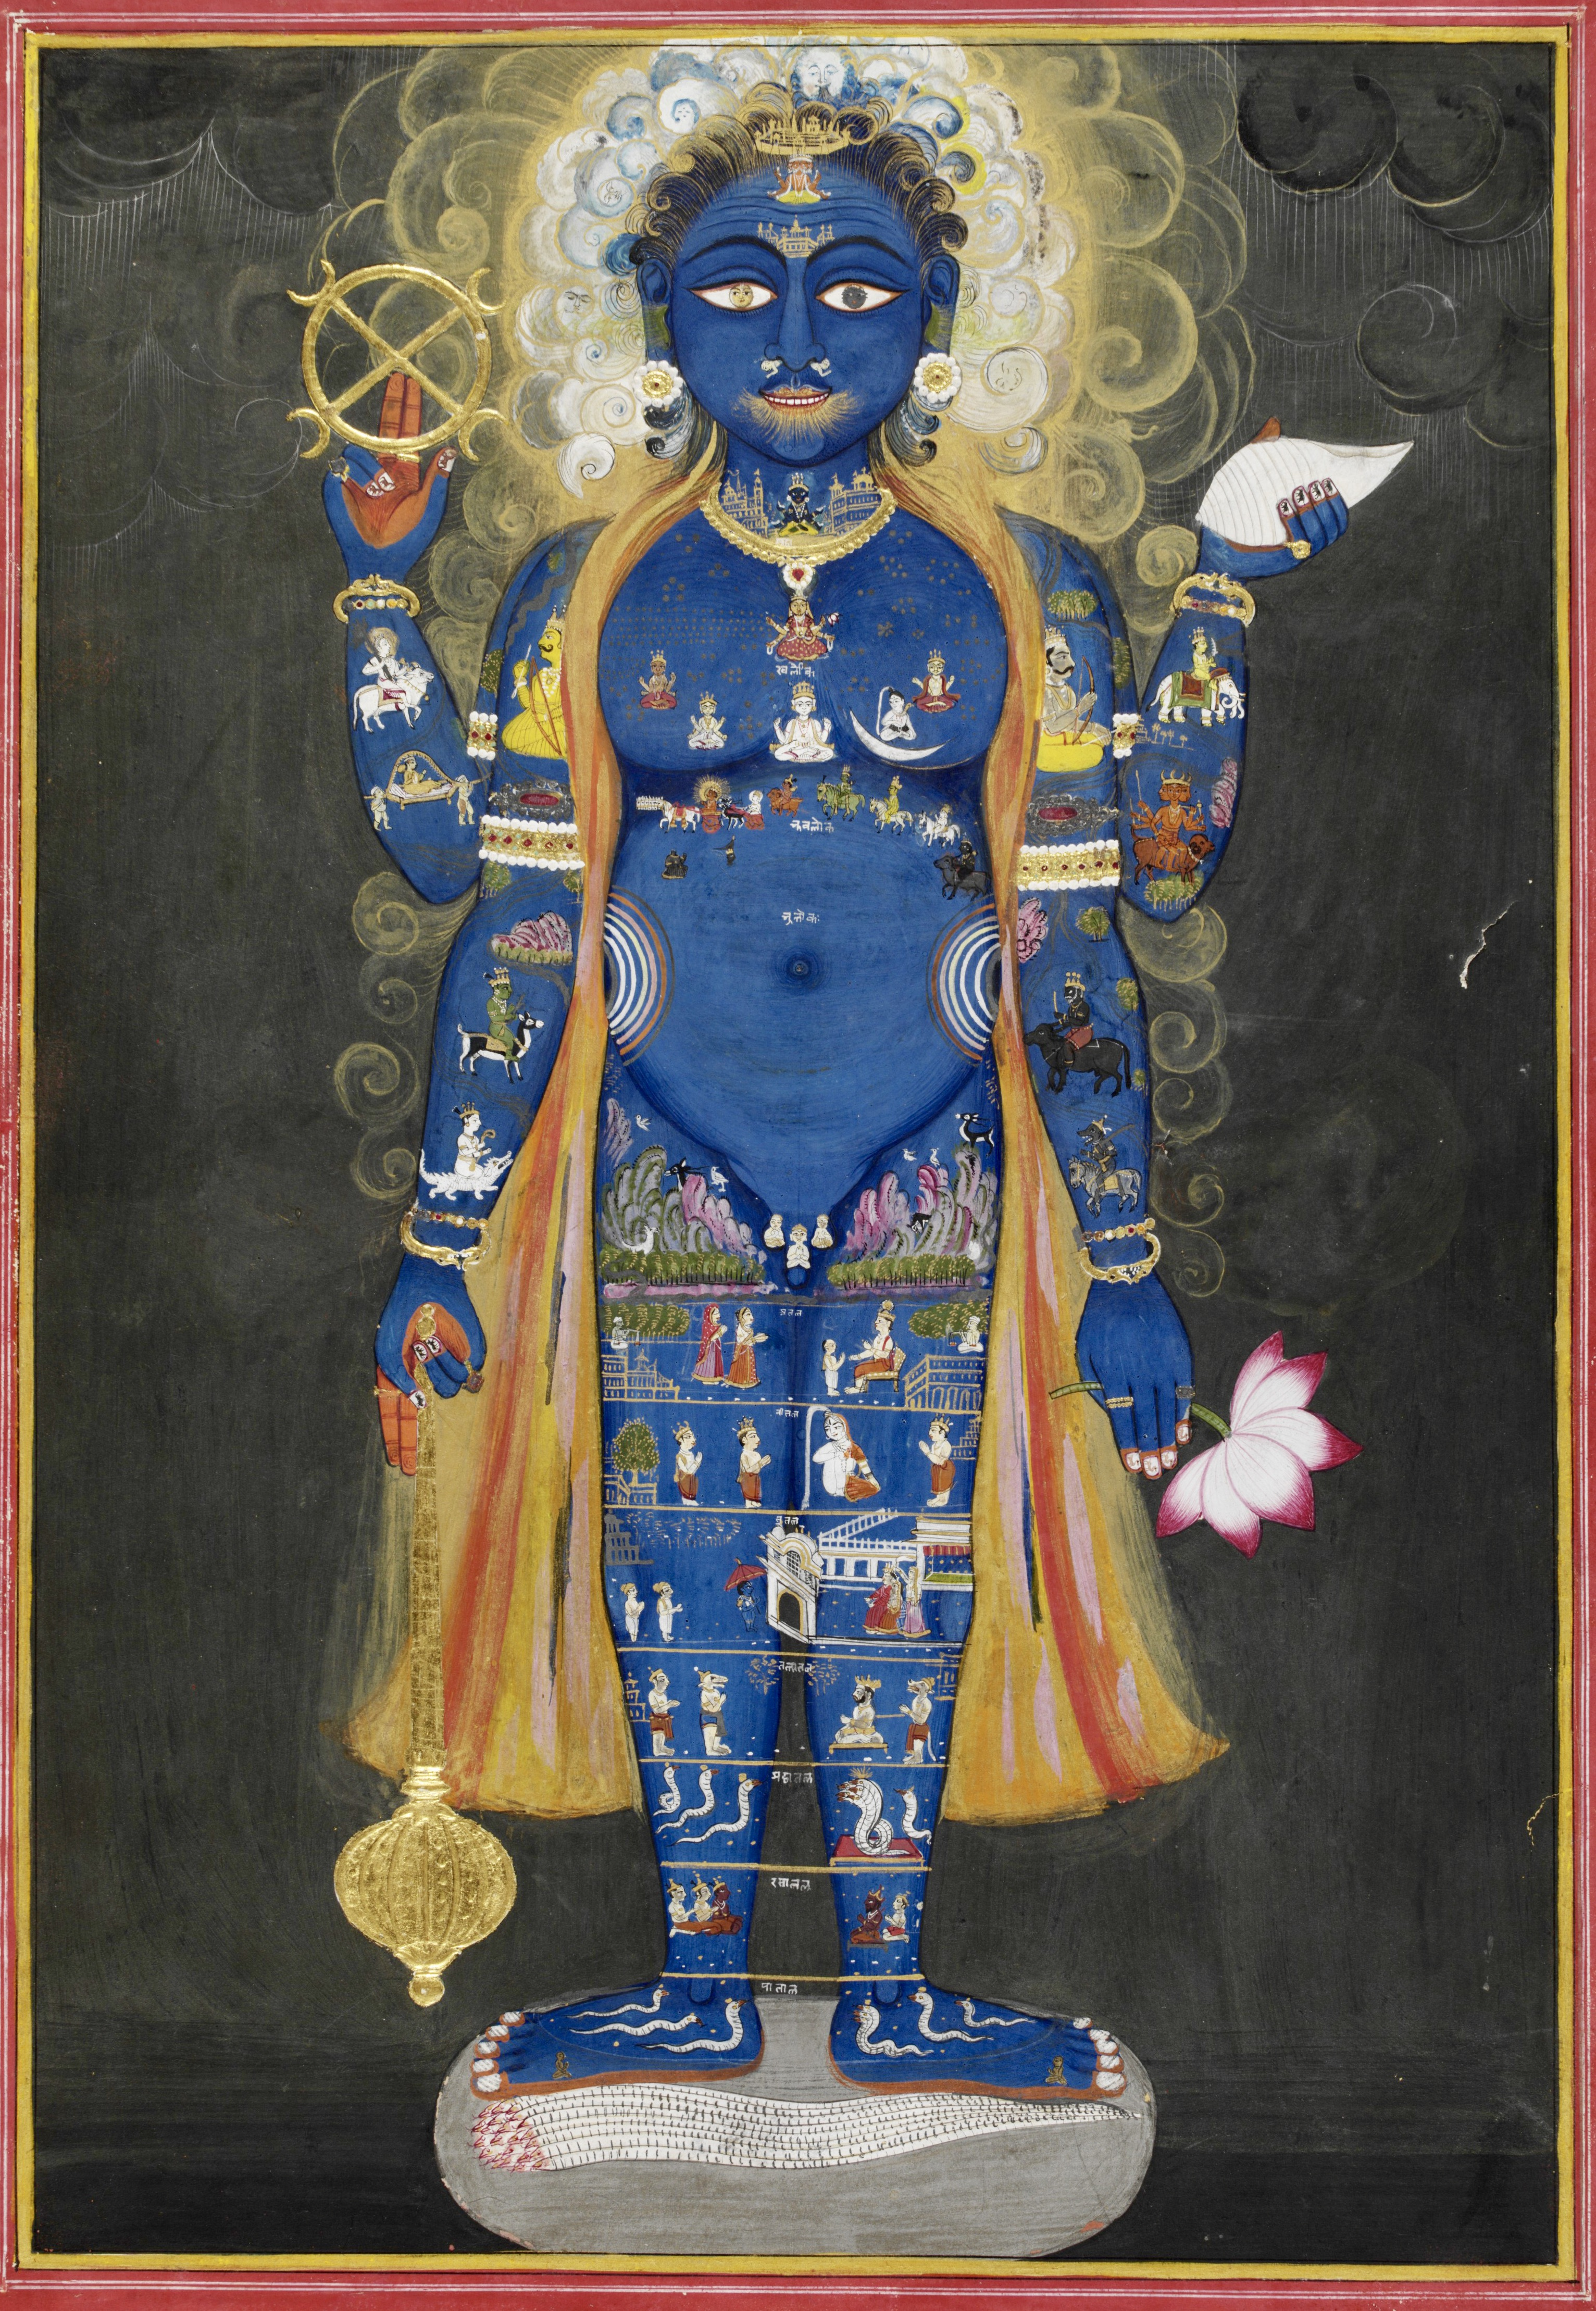
\includegraphics[width=1\textwidth]{pics/Vishnu_Vishvarupa_cropped.jpg}
	\caption{Viṣṇu Viśvarūpa, India, Rajasthan, Jaipur, ca. 1800–1820, Opaque watercolor and gold on paper, 38.5 × 28 cm, Victoria and Albert Museum, London, Given by Mrs. Gerald Clark.}
	\label{fig1}
      \end{figure}
\clearpage
  \begin{figure}[ht]
	\centering
  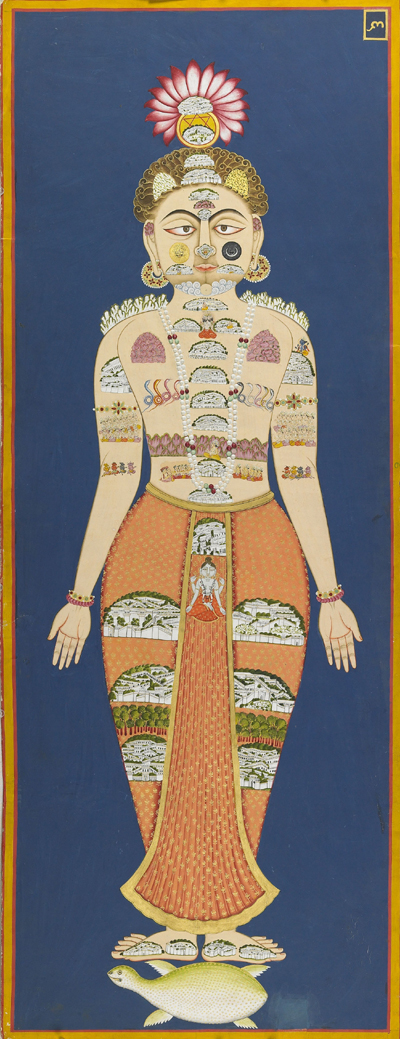
\includegraphics[width=0.5\textwidth]{pics/The_Equivalence_of_Self_and_Universe_(detail),_folio_6_from_the_Siddha_Siddhanta_Paddhati,_(Bulaki),_1824_(Samvat_1881);_122_x_46_cm._Mehrangarh_Museum_Trust..jpg}
	\caption{The Equivalence of Self and Universe (detail), folio 6 from the \textit{Siddhasiddhāntapaddhati} (Bulaki), India, Rajasthan, Jodhpur, 1824 (Samvat 1881), 122 x 46 cm, RJS 2378, Mehragarh Museum Trust.}
	\label{fig2}
      \end{figure}
      % \end{landscape}


\chapter{Bibliography}
 \label{sec:bibli}
   \clearpage
\newpage 
\thispagestyle{empty}
\quad  \addtocounter{page}{-1}

\printbibliography[heading=subbibintoc, title=Consulted Manuscripts, keyword=codex]

\printbibliography[heading=subbibintoc, title=Printed Editions, keyword=printsource]

\printbibliography[heading=subbibintoc, title=Secondary Literature, keyword=seclit]

\printbibliography[heading=subbibintoc, title=Online Sources, keyword=onlinesource]

\end{document}
